\documentclass[twoside]{book}

% Packages required by doxygen
\usepackage{fixltx2e}
\usepackage{calc}
\usepackage{doxygen}
\usepackage[export]{adjustbox} % also loads graphicx
\usepackage{graphicx}
\usepackage[utf8]{inputenc}
\usepackage{makeidx}
\usepackage{multicol}
\usepackage{multirow}
\PassOptionsToPackage{warn}{textcomp}
\usepackage{textcomp}
\usepackage[nointegrals]{wasysym}
\usepackage[table]{xcolor}

% Font selection
\usepackage[T1]{fontenc}
\usepackage[scaled=.90]{helvet}
\usepackage{courier}
\usepackage{amssymb}
\usepackage{sectsty}
\renewcommand{\familydefault}{\sfdefault}
\allsectionsfont{%
  \fontseries{bc}\selectfont%
  \color{darkgray}%
}
\renewcommand{\DoxyLabelFont}{%
  \fontseries{bc}\selectfont%
  \color{darkgray}%
}
\newcommand{\+}{\discretionary{\mbox{\scriptsize$\hookleftarrow$}}{}{}}

% Page & text layout
\usepackage{geometry}
\geometry{%
  a4paper,%
  top=2.5cm,%
  bottom=2.5cm,%
  left=2.5cm,%
  right=2.5cm%
}
\tolerance=750
\hfuzz=15pt
\hbadness=750
\setlength{\emergencystretch}{15pt}
\setlength{\parindent}{0cm}
\setlength{\parskip}{3ex plus 2ex minus 2ex}
\makeatletter
\renewcommand{\paragraph}{%
  \@startsection{paragraph}{4}{0ex}{-1.0ex}{1.0ex}{%
    \normalfont\normalsize\bfseries\SS@parafont%
  }%
}
\renewcommand{\subparagraph}{%
  \@startsection{subparagraph}{5}{0ex}{-1.0ex}{1.0ex}{%
    \normalfont\normalsize\bfseries\SS@subparafont%
  }%
}
\makeatother

% Headers & footers
\usepackage{fancyhdr}
\pagestyle{fancyplain}
\fancyhead[LE]{\fancyplain{}{\bfseries\thepage}}
\fancyhead[CE]{\fancyplain{}{}}
\fancyhead[RE]{\fancyplain{}{\bfseries\leftmark}}
\fancyhead[LO]{\fancyplain{}{\bfseries\rightmark}}
\fancyhead[CO]{\fancyplain{}{}}
\fancyhead[RO]{\fancyplain{}{\bfseries\thepage}}
\fancyfoot[LE]{\fancyplain{}{}}
\fancyfoot[CE]{\fancyplain{}{}}
\fancyfoot[RE]{\fancyplain{}{\bfseries\scriptsize Generated by Doxygen }}
\fancyfoot[LO]{\fancyplain{}{\bfseries\scriptsize Generated by Doxygen }}
\fancyfoot[CO]{\fancyplain{}{}}
\fancyfoot[RO]{\fancyplain{}{}}
\renewcommand{\footrulewidth}{0.4pt}
\renewcommand{\chaptermark}[1]{%
  \markboth{#1}{}%
}
\renewcommand{\sectionmark}[1]{%
  \markright{\thesection\ #1}%
}

% Indices & bibliography
\usepackage{natbib}
\usepackage[titles]{tocloft}
\setcounter{tocdepth}{3}
\setcounter{secnumdepth}{5}
\makeindex

% Hyperlinks (required, but should be loaded last)
\usepackage{ifpdf}
\ifpdf
  \usepackage[pdftex,pagebackref=true]{hyperref}
\else
  \usepackage[ps2pdf,pagebackref=true]{hyperref}
\fi
\hypersetup{%
  colorlinks=true,%
  linkcolor=blue,%
  citecolor=blue,%
  unicode%
}

% Custom commands
\newcommand{\clearemptydoublepage}{%
  \newpage{\pagestyle{empty}\cleardoublepage}%
}

\usepackage{caption}
\captionsetup{labelsep=space,justification=centering,font={bf},singlelinecheck=off,skip=4pt,position=top}

%===== C O N T E N T S =====

\begin{document}

% Titlepage & ToC
\hypersetup{pageanchor=false,
             bookmarksnumbered=true,
             pdfencoding=unicode
            }
\pagenumbering{alph}
\begin{titlepage}
\vspace*{7cm}
\begin{center}%
{\Large cylinder\+Flow \\[1ex]\large 1.\+0 }\\
\vspace*{1cm}
{\large Generated by Doxygen 1.8.14}\\
\end{center}
\end{titlepage}
\clearemptydoublepage
\pagenumbering{roman}
\tableofcontents
\clearemptydoublepage
\pagenumbering{arabic}
\hypersetup{pageanchor=true}

%--- Begin generated contents ---
\chapter{Todo List}
\label{todo}
\Hypertarget{todo}

\begin{DoxyRefList}
\item[\label{todo__todo000006}%
\Hypertarget{todo__todo000006}%
Member \mbox{\hyperlink{class_facet_acfcdcc63ac32fc2a1d0378a899441bbc}{Facet\+:\+:Facet}} (double a)]Need to restructure some \mbox{\hyperlink{class_mesh}{Mesh}} architecture to prevent the need for this constructor.  
\item[\label{todo__todo000007}%
\Hypertarget{todo__todo000007}%
Member \mbox{\hyperlink{class_facet_aaecf4566bbdbfb3904d9c3ce6f7c41cf}{Facet\+:\+:Facet}} (std\+::vector$<$ Node $\ast$$>$ node\+List)]provide checks within this constructor to either block node\+List.\+size() != 3 or generalize the \mbox{\hyperlink{class_facet}{Facet}} code to allow for arbitrary polygons as \mbox{\hyperlink{class_facet}{Facet}} objects.  
\item[\label{todo__todo000001}%
\Hypertarget{todo__todo000001}%
Class \mbox{\hyperlink{class_math_1_1_basis_rep}{Math\+:\+:Basis\+Rep}} ]Re-\/evaluate appropriateness of this class\textquotesingle{} inheritance from \mbox{\hyperlink{class_math_1_1_function}{Function}} class; it seems inappropriate. Intuitively, a basis element representation/decomposition should really just be a list of \mbox{\hyperlink{class_math_1_1_basis_el}{Basis\+El}} objects along with corresponding scalar coefficients.  
\item[\label{todo__todo000002}%
\Hypertarget{todo__todo000002}%
Member \mbox{\hyperlink{class_math_1_1_combinatorics_a174253b11651917aab46bc879449e59b}{Math\+:\+:Combinatorics\+:\+:testn\+Choosek}} (void)]Implement automatic testing of the n\+Choosek operation  
\item[\label{todo__todo000003}%
\Hypertarget{todo__todo000003}%
Member \mbox{\hyperlink{class_math_1_1_function_a97e51108b0374f8adc7982f92af4d0de}{Math\+:\+:Function\+:\+:Function}} ()]Implement a constructor with the specified parameters  
\item[\label{todo__todo000004}%
\Hypertarget{todo__todo000004}%
Member \mbox{\hyperlink{class_math_1_1_function_ad85e716accc64c1ea4962c828c4e216c}{Math\+:\+:Function\+:\+:integrate\+On\+Domain}} (void)]Method is currently not implemented  
\item[\label{todo__todo000005}%
\Hypertarget{todo__todo000005}%
Class \mbox{\hyperlink{class_mesh}{Mesh}} ]Allow for constrained DT 
\end{DoxyRefList}
\chapter{Namespace Index}
\section{Namespace List}
Here is a list of all namespaces with brief descriptions\+:\begin{DoxyCompactList}
\item\contentsline{section}{\mbox{\hyperlink{namespacecfgui}{cfgui}} }{\pageref{namespacecfgui}}{}
\item\contentsline{section}{\mbox{\hyperlink{namespace_math}{Math}} }{\pageref{namespace_math}}{}
\end{DoxyCompactList}

\chapter{Hierarchical Index}
\section{Class Hierarchy}
This inheritance list is sorted roughly, but not completely, alphabetically\+:\begin{DoxyCompactList}
\item \contentsline{section}{class\+Instance\+Counter$<$ T $>$}{\pageref{classclass_instance_counter}}{}
\item \contentsline{section}{class\+Instance\+Counter$<$ Facet $>$}{\pageref{classclass_instance_counter}}{}
\begin{DoxyCompactList}
\item \contentsline{section}{Facet}{\pageref{class_facet}}{}
\end{DoxyCompactList}
\item \contentsline{section}{class\+Instance\+Counter$<$ Node $>$}{\pageref{classclass_instance_counter}}{}
\begin{DoxyCompactList}
\item \contentsline{section}{Node}{\pageref{class_node}}{}
\end{DoxyCompactList}
\item \contentsline{section}{Math\+:\+:Combinatorics}{\pageref{class_math_1_1_combinatorics}}{}
\item \contentsline{section}{Math\+:\+:Function}{\pageref{class_math_1_1_function}}{}
\begin{DoxyCompactList}
\item \contentsline{section}{Math\+:\+:Basis\+El}{\pageref{class_math_1_1_basis_el}}{}
\item \contentsline{section}{Math\+:\+:Basis\+Rep}{\pageref{class_math_1_1_basis_rep}}{}
\end{DoxyCompactList}
\item \contentsline{section}{Matrix}{\pageref{class_matrix}}{}
\item \contentsline{section}{Mesh}{\pageref{class_mesh}}{}
\begin{DoxyCompactList}
\item \contentsline{section}{F\+E\+Mesh}{\pageref{class_f_e_mesh}}{}
\end{DoxyCompactList}
\item \contentsline{section}{Options}{\pageref{class_options}}{}
\item \contentsline{section}{Solver\+Base}{\pageref{class_solver_base}}{}
\begin{DoxyCompactList}
\item \contentsline{section}{Solver\+Euler}{\pageref{class_solver_euler}}{}
\item \contentsline{section}{Solver\+Poisson}{\pageref{class_solver_poisson}}{}
\end{DoxyCompactList}
\end{DoxyCompactList}

\chapter{Class Index}
\section{Class List}
Here are the classes, structs, unions and interfaces with brief descriptions\+:\begin{DoxyCompactList}
\item\contentsline{section}{\mbox{\hyperlink{class_math_1_1_basis_el}{Math\+::\+Basis\+El}} \\*Basis element class }{\pageref{class_math_1_1_basis_el}}{}
\item\contentsline{section}{\mbox{\hyperlink{class_math_1_1_basis_rep}{Math\+::\+Basis\+Rep}} \\*Basis element representation of a function }{\pageref{class_math_1_1_basis_rep}}{}
\item\contentsline{section}{\mbox{\hyperlink{classclass_instance_counter}{class\+Instance\+Counter$<$ T $>$}} \\*Class that tracks number of instatiated objects of type T during program execution }{\pageref{classclass_instance_counter}}{}
\item\contentsline{section}{\mbox{\hyperlink{class_math_1_1_combinatorics}{Math\+::\+Combinatorics}} \\*\mbox{\hyperlink{class_math_1_1_combinatorics}{Combinatorics}} class performs basic combinatorial operations }{\pageref{class_math_1_1_combinatorics}}{}
\item\contentsline{section}{\mbox{\hyperlink{class_facet}{Facet}} \\*\mbox{\hyperlink{class_facet}{Facet}} object is a triangle defined by three \mbox{\hyperlink{class_node}{Node}} objects }{\pageref{class_facet}}{}
\item\contentsline{section}{\mbox{\hyperlink{class_f_e_mesh}{F\+E\+Mesh}} }{\pageref{class_f_e_mesh}}{}
\item\contentsline{section}{\mbox{\hyperlink{class_math_1_1_function}{Math\+::\+Function}} \\*This class associates a list of }{\pageref{class_math_1_1_function}}{}
\item\contentsline{section}{\mbox{\hyperlink{class_matrix}{Matrix}} }{\pageref{class_matrix}}{}
\item\contentsline{section}{\mbox{\hyperlink{class_mesh}{Mesh}} \\*\mbox{\hyperlink{class_mesh}{Mesh}} class generates and stores a 2D mesh from an input grid points file }{\pageref{class_mesh}}{}
\item\contentsline{section}{\mbox{\hyperlink{class_node}{Node}} \\*\mbox{\hyperlink{class_node}{Node}} class provides A\+PI for a vertex object in a \mbox{\hyperlink{class_mesh}{Mesh}} }{\pageref{class_node}}{}
\item\contentsline{section}{\mbox{\hyperlink{class_options}{Options}} }{\pageref{class_options}}{}
\item\contentsline{section}{\mbox{\hyperlink{class_solver_base}{Solver\+Base}} }{\pageref{class_solver_base}}{}
\item\contentsline{section}{\mbox{\hyperlink{class_solver_euler}{Solver\+Euler}} }{\pageref{class_solver_euler}}{}
\item\contentsline{section}{\mbox{\hyperlink{class_solver_poisson}{Solver\+Poisson}} }{\pageref{class_solver_poisson}}{}
\end{DoxyCompactList}

\chapter{File Index}
\section{File List}
Here is a list of all files with brief descriptions\+:\begin{DoxyCompactList}
\item\contentsline{section}{\mbox{\hyperlink{cfgui_8py}{cfgui.\+py}} }{\pageref{cfgui_8py}}{}
\item\contentsline{section}{\mbox{\hyperlink{_f_e_mesh_8cpp}{F\+E\+Mesh.\+cpp}} }{\pageref{_f_e_mesh_8cpp}}{}
\item\contentsline{section}{\mbox{\hyperlink{_f_e_mesh_8hpp}{F\+E\+Mesh.\+hpp}} }{\pageref{_f_e_mesh_8hpp}}{}
\item\contentsline{section}{\mbox{\hyperlink{_includes_8hpp}{Includes.\+hpp}} }{\pageref{_includes_8hpp}}{}
\item\contentsline{section}{\mbox{\hyperlink{main_8cpp}{main.\+cpp}} }{\pageref{main_8cpp}}{}
\item\contentsline{section}{\mbox{\hyperlink{_math_8cpp}{Math.\+cpp}} }{\pageref{_math_8cpp}}{}
\item\contentsline{section}{\mbox{\hyperlink{_math_8hpp}{Math.\+hpp}} }{\pageref{_math_8hpp}}{}
\item\contentsline{section}{\mbox{\hyperlink{_matrix_8cpp}{Matrix.\+cpp}} }{\pageref{_matrix_8cpp}}{}
\item\contentsline{section}{\mbox{\hyperlink{_matrix_8hpp}{Matrix.\+hpp}} }{\pageref{_matrix_8hpp}}{}
\item\contentsline{section}{\mbox{\hyperlink{_mesh_8cpp}{Mesh.\+cpp}} }{\pageref{_mesh_8cpp}}{}
\item\contentsline{section}{\mbox{\hyperlink{_mesh_8hpp}{Mesh.\+hpp}} }{\pageref{_mesh_8hpp}}{}
\item\contentsline{section}{\mbox{\hyperlink{_options_8cpp}{Options.\+cpp}} }{\pageref{_options_8cpp}}{}
\item\contentsline{section}{\mbox{\hyperlink{_options_8hpp}{Options.\+hpp}} }{\pageref{_options_8hpp}}{}
\item\contentsline{section}{\mbox{\hyperlink{_solver_8cpp}{Solver.\+cpp}} }{\pageref{_solver_8cpp}}{}
\item\contentsline{section}{\mbox{\hyperlink{_solver_8hpp}{Solver.\+hpp}} }{\pageref{_solver_8hpp}}{}
\item\contentsline{section}{\mbox{\hyperlink{_solver_euler_8cpp}{Solver\+Euler.\+cpp}} }{\pageref{_solver_euler_8cpp}}{}
\item\contentsline{section}{\mbox{\hyperlink{_solver_euler_8hpp}{Solver\+Euler.\+hpp}} }{\pageref{_solver_euler_8hpp}}{}
\item\contentsline{section}{\mbox{\hyperlink{_solver_poisson_8cpp}{Solver\+Poisson.\+cpp}} }{\pageref{_solver_poisson_8cpp}}{}
\item\contentsline{section}{\mbox{\hyperlink{_solver_poisson_8hpp}{Solver\+Poisson.\+hpp}} }{\pageref{_solver_poisson_8hpp}}{}
\item\contentsline{section}{\mbox{\hyperlink{_utilities_8hpp}{Utilities.\+hpp}} }{\pageref{_utilities_8hpp}}{}
\item\contentsline{section}{\mbox{\hyperlink{_vect_ops_8cpp}{Vect\+Ops.\+cpp}} }{\pageref{_vect_ops_8cpp}}{}
\item\contentsline{section}{\mbox{\hyperlink{_vect_ops_8hpp}{Vect\+Ops.\+hpp}} }{\pageref{_vect_ops_8hpp}}{}
\end{DoxyCompactList}

\chapter{Namespace Documentation}
\hypertarget{namespacecfgui}{}\section{cfgui Namespace Reference}
\label{namespacecfgui}\index{cfgui@{cfgui}}
\subsection*{Variables}
\begin{DoxyCompactItemize}
\item 
\mbox{\hyperlink{namespacecfgui_ad0261b0d3cca8159d011afa3c17bd9f1}{root}} = tk.\+Tk()
\item 
\mbox{\hyperlink{namespacecfgui_a64ae648845422a3c70e06f75eb5fa172}{f}} = Figure(figsize=(6,5), dpi=150)
\item 
\mbox{\hyperlink{namespacecfgui_afa1e0012aec603eb6c61806994452873}{a}} = f.\+add\+\_\+subplot(111)
\item 
string \mbox{\hyperlink{namespacecfgui_ae4078f684c5dfbf537a587c88b087e39}{filename}} = \char`\"{}\char`\"{}
\item 
string \mbox{\hyperlink{namespacecfgui_adacec56309d4b55d655ac53531223503}{newfilename}} = \char`\"{}\char`\"{}
\item 
int \mbox{\hyperlink{namespacecfgui_a4f032350a6dae97371e2e21bcc0223f3}{filehandle}} = 0
\item 
list \mbox{\hyperlink{namespacecfgui_a4d1fd2c1f28a077f91899b4af9665928}{active\+Node\+List}} = \mbox{[}$\,$\mbox{]}
\item 
int \mbox{\hyperlink{namespacecfgui_a69cb956a983205fbd404d059670db416}{new\+Node\+ID}} = 0
\item 
int \mbox{\hyperlink{namespacecfgui_ade4f0d3b0706b49e072673e48b2ac242}{unmeshed}} = 0
\item 
int \mbox{\hyperlink{namespacecfgui_aa3107f0b2f277f51f50bc28f5d93cb7e}{editing}} = 0
\item 
\mbox{\hyperlink{namespacecfgui_aafee5f0725f5961d2bc6696ddac838ce}{canvas}} = Figure\+Canvas\+Tk\+Agg(\mbox{\hyperlink{namespacecfgui_a64ae648845422a3c70e06f75eb5fa172}{f}}, master=\mbox{\hyperlink{namespacecfgui_ad0261b0d3cca8159d011afa3c17bd9f1}{root}})
\item 
\mbox{\hyperlink{namespacecfgui_ae9b6ae360c249a392d4154426dff9609}{side}}
\item 
\mbox{\hyperlink{namespacecfgui_abdd84db69f76172a7b2e574cf726eb24}{T\+OP}}
\item 
\mbox{\hyperlink{namespacecfgui_a86a27e16bd39f4f3228f753b3f04cb91}{fill}}
\item 
\mbox{\hyperlink{namespacecfgui_ae68d5f9438e41baf4820d8044f868346}{B\+O\+TH}}
\item 
\mbox{\hyperlink{namespacecfgui_a584b910dd9e596e04fe616d866f91ff2}{expand}}
\item 
\mbox{\hyperlink{namespacecfgui_a7410773bac81022643bbb700b65ffd35}{toolbar}} = Navigation\+Toolbar2\+Tk\+Agg(\mbox{\hyperlink{namespacecfgui_aafee5f0725f5961d2bc6696ddac838ce}{canvas}},\mbox{\hyperlink{namespacecfgui_ad0261b0d3cca8159d011afa3c17bd9f1}{root}})
\item 
\mbox{\hyperlink{namespacecfgui_a178f690140e4928e80ed598ebbbf6ec1}{menu}} = Menu(\mbox{\hyperlink{namespacecfgui_ad0261b0d3cca8159d011afa3c17bd9f1}{root}})
\item 
\mbox{\hyperlink{namespacecfgui_ae54e3f8d355a03929c89a227c506d39e}{filemenu}} = Menu(\mbox{\hyperlink{namespacecfgui_a178f690140e4928e80ed598ebbbf6ec1}{menu}})
\item 
\mbox{\hyperlink{namespacecfgui_a5bb1e89c42bd42a9baf53da59a27658d}{label}}
\item 
\mbox{\hyperlink{namespacecfgui_a32a18002fc6635b3c814b5e9b329ec6b}{command}}
\item 
\mbox{\hyperlink{namespacecfgui_aa44f9f5c68e640ec65a1a1c93e148982}{accelerator}}
\item 
\mbox{\hyperlink{namespacecfgui_afef0987be82596ace82157e0682cac34}{editmenu}} = Menu(\mbox{\hyperlink{namespacecfgui_a178f690140e4928e80ed598ebbbf6ec1}{menu}})
\item 
\mbox{\hyperlink{namespacecfgui_a3a48ab8eff50c8134be0e6351bc9279d}{helpmenu}} = Menu(\mbox{\hyperlink{namespacecfgui_a178f690140e4928e80ed598ebbbf6ec1}{menu}})
\item 
\mbox{\hyperlink{namespacecfgui_a4cb6233c9db194dad78f3a686d22475c}{mesh\+Button}} = tk.\+Button(master=\mbox{\hyperlink{namespacecfgui_ad0261b0d3cca8159d011afa3c17bd9f1}{root}}, text=\char`\"{}Mesh (\%s\%s)\char`\"{} \% (u\char`\"{}\textbackslash{}u2318\char`\"{},\char`\"{}M\char`\"{}), command=\+\_\+mesh)
\end{DoxyCompactItemize}


\subsection{Variable Documentation}
\mbox{\Hypertarget{namespacecfgui_afa1e0012aec603eb6c61806994452873}\label{namespacecfgui_afa1e0012aec603eb6c61806994452873}} 
\index{cfgui@{cfgui}!a@{a}}
\index{a@{a}!cfgui@{cfgui}}
\subsubsection{\texorpdfstring{a}{a}}
{\footnotesize\ttfamily cfgui.\+a = f.\+add\+\_\+subplot(111)}

\mbox{\Hypertarget{namespacecfgui_aa44f9f5c68e640ec65a1a1c93e148982}\label{namespacecfgui_aa44f9f5c68e640ec65a1a1c93e148982}} 
\index{cfgui@{cfgui}!accelerator@{accelerator}}
\index{accelerator@{accelerator}!cfgui@{cfgui}}
\subsubsection{\texorpdfstring{accelerator}{accelerator}}
{\footnotesize\ttfamily cfgui.\+accelerator}

\mbox{\Hypertarget{namespacecfgui_a4d1fd2c1f28a077f91899b4af9665928}\label{namespacecfgui_a4d1fd2c1f28a077f91899b4af9665928}} 
\index{cfgui@{cfgui}!active\+Node\+List@{active\+Node\+List}}
\index{active\+Node\+List@{active\+Node\+List}!cfgui@{cfgui}}
\subsubsection{\texorpdfstring{active\+Node\+List}{activeNodeList}}
{\footnotesize\ttfamily list cfgui.\+active\+Node\+List = \mbox{[}$\,$\mbox{]}}

\mbox{\Hypertarget{namespacecfgui_ae68d5f9438e41baf4820d8044f868346}\label{namespacecfgui_ae68d5f9438e41baf4820d8044f868346}} 
\index{cfgui@{cfgui}!B\+O\+TH@{B\+O\+TH}}
\index{B\+O\+TH@{B\+O\+TH}!cfgui@{cfgui}}
\subsubsection{\texorpdfstring{B\+O\+TH}{BOTH}}
{\footnotesize\ttfamily cfgui.\+B\+O\+TH}

\mbox{\Hypertarget{namespacecfgui_aafee5f0725f5961d2bc6696ddac838ce}\label{namespacecfgui_aafee5f0725f5961d2bc6696ddac838ce}} 
\index{cfgui@{cfgui}!canvas@{canvas}}
\index{canvas@{canvas}!cfgui@{cfgui}}
\subsubsection{\texorpdfstring{canvas}{canvas}}
{\footnotesize\ttfamily cfgui.\+canvas = Figure\+Canvas\+Tk\+Agg(\mbox{\hyperlink{namespacecfgui_a64ae648845422a3c70e06f75eb5fa172}{f}}, master=\mbox{\hyperlink{namespacecfgui_ad0261b0d3cca8159d011afa3c17bd9f1}{root}})}

\mbox{\Hypertarget{namespacecfgui_a32a18002fc6635b3c814b5e9b329ec6b}\label{namespacecfgui_a32a18002fc6635b3c814b5e9b329ec6b}} 
\index{cfgui@{cfgui}!command@{command}}
\index{command@{command}!cfgui@{cfgui}}
\subsubsection{\texorpdfstring{command}{command}}
{\footnotesize\ttfamily cfgui.\+command}

\mbox{\Hypertarget{namespacecfgui_aa3107f0b2f277f51f50bc28f5d93cb7e}\label{namespacecfgui_aa3107f0b2f277f51f50bc28f5d93cb7e}} 
\index{cfgui@{cfgui}!editing@{editing}}
\index{editing@{editing}!cfgui@{cfgui}}
\subsubsection{\texorpdfstring{editing}{editing}}
{\footnotesize\ttfamily int cfgui.\+editing = 0}

\mbox{\Hypertarget{namespacecfgui_afef0987be82596ace82157e0682cac34}\label{namespacecfgui_afef0987be82596ace82157e0682cac34}} 
\index{cfgui@{cfgui}!editmenu@{editmenu}}
\index{editmenu@{editmenu}!cfgui@{cfgui}}
\subsubsection{\texorpdfstring{editmenu}{editmenu}}
{\footnotesize\ttfamily cfgui.\+editmenu = Menu(\mbox{\hyperlink{namespacecfgui_a178f690140e4928e80ed598ebbbf6ec1}{menu}})}

\mbox{\Hypertarget{namespacecfgui_a584b910dd9e596e04fe616d866f91ff2}\label{namespacecfgui_a584b910dd9e596e04fe616d866f91ff2}} 
\index{cfgui@{cfgui}!expand@{expand}}
\index{expand@{expand}!cfgui@{cfgui}}
\subsubsection{\texorpdfstring{expand}{expand}}
{\footnotesize\ttfamily cfgui.\+expand}

\mbox{\Hypertarget{namespacecfgui_a64ae648845422a3c70e06f75eb5fa172}\label{namespacecfgui_a64ae648845422a3c70e06f75eb5fa172}} 
\index{cfgui@{cfgui}!f@{f}}
\index{f@{f}!cfgui@{cfgui}}
\subsubsection{\texorpdfstring{f}{f}}
{\footnotesize\ttfamily cfgui.\+f = Figure(figsize=(6,5), dpi=150)}

\mbox{\Hypertarget{namespacecfgui_a4f032350a6dae97371e2e21bcc0223f3}\label{namespacecfgui_a4f032350a6dae97371e2e21bcc0223f3}} 
\index{cfgui@{cfgui}!filehandle@{filehandle}}
\index{filehandle@{filehandle}!cfgui@{cfgui}}
\subsubsection{\texorpdfstring{filehandle}{filehandle}}
{\footnotesize\ttfamily int cfgui.\+filehandle = 0}

\mbox{\Hypertarget{namespacecfgui_ae54e3f8d355a03929c89a227c506d39e}\label{namespacecfgui_ae54e3f8d355a03929c89a227c506d39e}} 
\index{cfgui@{cfgui}!filemenu@{filemenu}}
\index{filemenu@{filemenu}!cfgui@{cfgui}}
\subsubsection{\texorpdfstring{filemenu}{filemenu}}
{\footnotesize\ttfamily cfgui.\+filemenu = Menu(\mbox{\hyperlink{namespacecfgui_a178f690140e4928e80ed598ebbbf6ec1}{menu}})}

\mbox{\Hypertarget{namespacecfgui_ae4078f684c5dfbf537a587c88b087e39}\label{namespacecfgui_ae4078f684c5dfbf537a587c88b087e39}} 
\index{cfgui@{cfgui}!filename@{filename}}
\index{filename@{filename}!cfgui@{cfgui}}
\subsubsection{\texorpdfstring{filename}{filename}}
{\footnotesize\ttfamily string cfgui.\+filename = \char`\"{}\char`\"{}}

\mbox{\Hypertarget{namespacecfgui_a86a27e16bd39f4f3228f753b3f04cb91}\label{namespacecfgui_a86a27e16bd39f4f3228f753b3f04cb91}} 
\index{cfgui@{cfgui}!fill@{fill}}
\index{fill@{fill}!cfgui@{cfgui}}
\subsubsection{\texorpdfstring{fill}{fill}}
{\footnotesize\ttfamily cfgui.\+fill}

\mbox{\Hypertarget{namespacecfgui_a3a48ab8eff50c8134be0e6351bc9279d}\label{namespacecfgui_a3a48ab8eff50c8134be0e6351bc9279d}} 
\index{cfgui@{cfgui}!helpmenu@{helpmenu}}
\index{helpmenu@{helpmenu}!cfgui@{cfgui}}
\subsubsection{\texorpdfstring{helpmenu}{helpmenu}}
{\footnotesize\ttfamily cfgui.\+helpmenu = Menu(\mbox{\hyperlink{namespacecfgui_a178f690140e4928e80ed598ebbbf6ec1}{menu}})}

\mbox{\Hypertarget{namespacecfgui_a5bb1e89c42bd42a9baf53da59a27658d}\label{namespacecfgui_a5bb1e89c42bd42a9baf53da59a27658d}} 
\index{cfgui@{cfgui}!label@{label}}
\index{label@{label}!cfgui@{cfgui}}
\subsubsection{\texorpdfstring{label}{label}}
{\footnotesize\ttfamily cfgui.\+label}

\mbox{\Hypertarget{namespacecfgui_a178f690140e4928e80ed598ebbbf6ec1}\label{namespacecfgui_a178f690140e4928e80ed598ebbbf6ec1}} 
\index{cfgui@{cfgui}!menu@{menu}}
\index{menu@{menu}!cfgui@{cfgui}}
\subsubsection{\texorpdfstring{menu}{menu}}
{\footnotesize\ttfamily cfgui.\+menu = Menu(\mbox{\hyperlink{namespacecfgui_ad0261b0d3cca8159d011afa3c17bd9f1}{root}})}

\mbox{\Hypertarget{namespacecfgui_a4cb6233c9db194dad78f3a686d22475c}\label{namespacecfgui_a4cb6233c9db194dad78f3a686d22475c}} 
\index{cfgui@{cfgui}!mesh\+Button@{mesh\+Button}}
\index{mesh\+Button@{mesh\+Button}!cfgui@{cfgui}}
\subsubsection{\texorpdfstring{mesh\+Button}{meshButton}}
{\footnotesize\ttfamily cfgui.\+mesh\+Button = tk.\+Button(master=\mbox{\hyperlink{namespacecfgui_ad0261b0d3cca8159d011afa3c17bd9f1}{root}}, text=\char`\"{}Mesh (\%s\%s)\char`\"{} \% (u\char`\"{}\textbackslash{}u2318\char`\"{},\char`\"{}M\char`\"{}), command=\+\_\+mesh)}

\mbox{\Hypertarget{namespacecfgui_adacec56309d4b55d655ac53531223503}\label{namespacecfgui_adacec56309d4b55d655ac53531223503}} 
\index{cfgui@{cfgui}!newfilename@{newfilename}}
\index{newfilename@{newfilename}!cfgui@{cfgui}}
\subsubsection{\texorpdfstring{newfilename}{newfilename}}
{\footnotesize\ttfamily string cfgui.\+newfilename = \char`\"{}\char`\"{}}

\mbox{\Hypertarget{namespacecfgui_a69cb956a983205fbd404d059670db416}\label{namespacecfgui_a69cb956a983205fbd404d059670db416}} 
\index{cfgui@{cfgui}!new\+Node\+ID@{new\+Node\+ID}}
\index{new\+Node\+ID@{new\+Node\+ID}!cfgui@{cfgui}}
\subsubsection{\texorpdfstring{new\+Node\+ID}{newNodeID}}
{\footnotesize\ttfamily int cfgui.\+new\+Node\+ID = 0}

\mbox{\Hypertarget{namespacecfgui_ad0261b0d3cca8159d011afa3c17bd9f1}\label{namespacecfgui_ad0261b0d3cca8159d011afa3c17bd9f1}} 
\index{cfgui@{cfgui}!root@{root}}
\index{root@{root}!cfgui@{cfgui}}
\subsubsection{\texorpdfstring{root}{root}}
{\footnotesize\ttfamily cfgui.\+root = tk.\+Tk()}

\mbox{\Hypertarget{namespacecfgui_ae9b6ae360c249a392d4154426dff9609}\label{namespacecfgui_ae9b6ae360c249a392d4154426dff9609}} 
\index{cfgui@{cfgui}!side@{side}}
\index{side@{side}!cfgui@{cfgui}}
\subsubsection{\texorpdfstring{side}{side}}
{\footnotesize\ttfamily cfgui.\+side}

\mbox{\Hypertarget{namespacecfgui_a7410773bac81022643bbb700b65ffd35}\label{namespacecfgui_a7410773bac81022643bbb700b65ffd35}} 
\index{cfgui@{cfgui}!toolbar@{toolbar}}
\index{toolbar@{toolbar}!cfgui@{cfgui}}
\subsubsection{\texorpdfstring{toolbar}{toolbar}}
{\footnotesize\ttfamily cfgui.\+toolbar = Navigation\+Toolbar2\+Tk\+Agg(\mbox{\hyperlink{namespacecfgui_aafee5f0725f5961d2bc6696ddac838ce}{canvas}},\mbox{\hyperlink{namespacecfgui_ad0261b0d3cca8159d011afa3c17bd9f1}{root}})}

\mbox{\Hypertarget{namespacecfgui_abdd84db69f76172a7b2e574cf726eb24}\label{namespacecfgui_abdd84db69f76172a7b2e574cf726eb24}} 
\index{cfgui@{cfgui}!T\+OP@{T\+OP}}
\index{T\+OP@{T\+OP}!cfgui@{cfgui}}
\subsubsection{\texorpdfstring{T\+OP}{TOP}}
{\footnotesize\ttfamily cfgui.\+T\+OP}

\mbox{\Hypertarget{namespacecfgui_ade4f0d3b0706b49e072673e48b2ac242}\label{namespacecfgui_ade4f0d3b0706b49e072673e48b2ac242}} 
\index{cfgui@{cfgui}!unmeshed@{unmeshed}}
\index{unmeshed@{unmeshed}!cfgui@{cfgui}}
\subsubsection{\texorpdfstring{unmeshed}{unmeshed}}
{\footnotesize\ttfamily int cfgui.\+unmeshed = 0}


\hypertarget{namespace_math}{}\section{Math Namespace Reference}
\label{namespace_math}\index{Math@{Math}}
\subsection*{Classes}
\begin{DoxyCompactItemize}
\item 
class \mbox{\hyperlink{class_math_1_1_basis_el}{Basis\+El}}
\begin{DoxyCompactList}\small\item\em Basis element class. \end{DoxyCompactList}\item 
class \mbox{\hyperlink{class_math_1_1_basis_rep}{Basis\+Rep}}
\begin{DoxyCompactList}\small\item\em Basis element representation of a function. \end{DoxyCompactList}\item 
class \mbox{\hyperlink{class_math_1_1_combinatorics}{Combinatorics}}
\begin{DoxyCompactList}\small\item\em \mbox{\hyperlink{class_math_1_1_combinatorics}{Combinatorics}} class performs basic combinatorial operations. \end{DoxyCompactList}\item 
class \mbox{\hyperlink{class_math_1_1_function}{Function}}
\begin{DoxyCompactList}\small\item\em This class associates a list of. \end{DoxyCompactList}\end{DoxyCompactItemize}


\subsection{Detailed Description}
This namespace contains some helpful mathematical objects and operations 
\chapter{Class Documentation}
\hypertarget{class_math_1_1_basis_el}{}\section{Math\+:\+:Basis\+El Class Reference}
\label{class_math_1_1_basis_el}\index{Math\+::\+Basis\+El@{Math\+::\+Basis\+El}}


Basis element class.  


Inheritance diagram for Math\+:\+:Basis\+El\+:\begin{figure}[H]
\begin{center}
\leavevmode
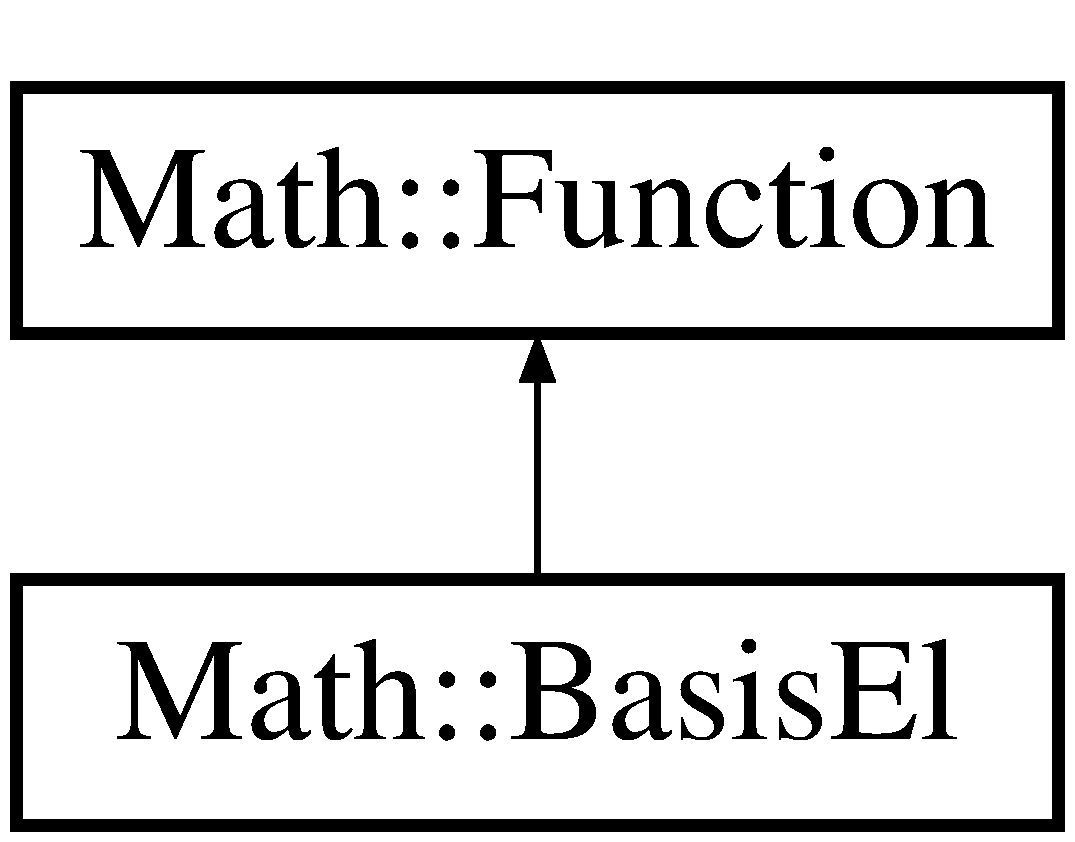
\includegraphics[height=2.000000cm]{class_math_1_1_basis_el}
\end{center}
\end{figure}
\subsection*{Additional Inherited Members}


\subsection{Detailed Description}
Basis element class. 

Basis element class is the building block of the finite element basis decomposition of a given function. 

The documentation for this class was generated from the following files\+:\begin{DoxyCompactItemize}
\item 
\mbox{\hyperlink{_math_8hpp}{Math.\+hpp}}\item 
\mbox{\hyperlink{_math_8cpp}{Math.\+cpp}}\end{DoxyCompactItemize}

\hypertarget{class_math_1_1_basis_rep}{}\section{Math\+:\+:Basis\+Rep Class Reference}
\label{class_math_1_1_basis_rep}\index{Math\+::\+Basis\+Rep@{Math\+::\+Basis\+Rep}}


Basis element representation of a function.  


Inheritance diagram for Math\+:\+:Basis\+Rep\+:\begin{figure}[H]
\begin{center}
\leavevmode
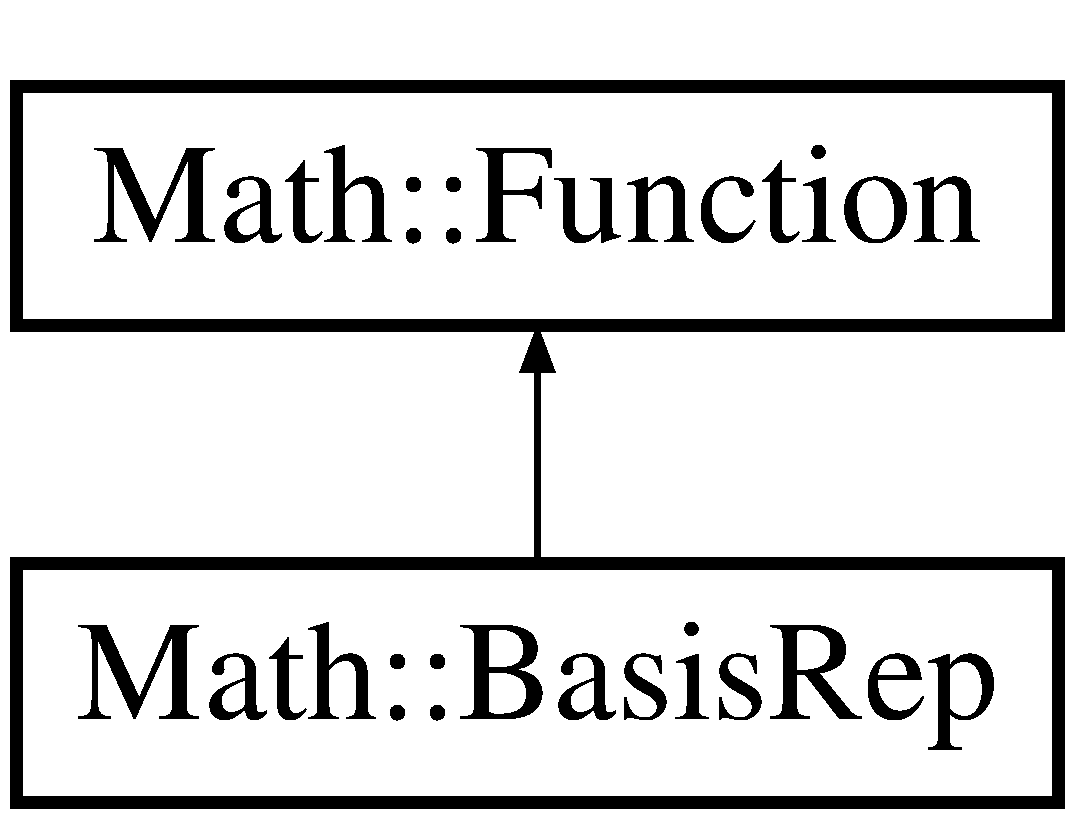
\includegraphics[height=2.000000cm]{class_math_1_1_basis_rep}
\end{center}
\end{figure}
\subsection*{Additional Inherited Members}


\subsection{Detailed Description}
Basis element representation of a function. 

This class stores a basis elemenet representation of a function. \begin{DoxyRefDesc}{Todo}
\item[\mbox{\hyperlink{todo__todo000001}{Todo}}]Re-\/evaluate appropriateness of this class\textquotesingle{} inheritance from \mbox{\hyperlink{class_math_1_1_function}{Function}} class; it seems inappropriate. Intuitively, a basis element representation/decomposition should really just be a list of \mbox{\hyperlink{class_math_1_1_basis_el}{Basis\+El}} objects along with corresponding scalar coefficients. \end{DoxyRefDesc}


The documentation for this class was generated from the following file\+:\begin{DoxyCompactItemize}
\item 
\mbox{\hyperlink{_math_8hpp}{Math.\+hpp}}\end{DoxyCompactItemize}

\hypertarget{classclass_instance_counter}{}\section{class\+Instance\+Counter$<$ T $>$ Class Template Reference}
\label{classclass_instance_counter}\index{class\+Instance\+Counter$<$ T $>$@{class\+Instance\+Counter$<$ T $>$}}


Class that tracks number of instatiated objects of type T during program execution.  


\subsection*{Public Member Functions}
\begin{DoxyCompactItemize}
\item 
\mbox{\hyperlink{classclass_instance_counter_a9d5f75752ecb644bd7e732a3b9d43702}{class\+Instance\+Counter}} ()
\begin{DoxyCompactList}\small\item\em The constructor increments the global variable ci\+Counter$<$\+T$>$ \end{DoxyCompactList}\item 
\mbox{\hyperlink{classclass_instance_counter_aa4bb00c47ae2c87fa51e447624361a0a}{$\sim$class\+Instance\+Counter}} ()
\begin{DoxyCompactList}\small\item\em The destructor decrements the global variable ci\+Counter$<$\+T$>$ \end{DoxyCompactList}\end{DoxyCompactItemize}
\subsection*{Static Protected Attributes}
\begin{DoxyCompactItemize}
\item 
static int \mbox{\hyperlink{classclass_instance_counter_a990f94f1650bb05ade3f4deba9110806}{ci\+Counter}} = 0
\begin{DoxyCompactList}\small\item\em $<$ Data member that tracks the number of instances of type {\bfseries T} \end{DoxyCompactList}\end{DoxyCompactItemize}


\subsection{Detailed Description}
\subsubsection*{template$<$class T$>$\newline
class class\+Instance\+Counter$<$ T $>$}

Class that tracks number of instatiated objects of type T during program execution. 

This templated class uses a global variable to track the number of instantiations of type {\bfseries T} through incrementing/decrementing the counter variable in the constructor/destructor, respectively. To track number of instances of a class of type {\bfseries T}, ensure that the class {\bfseries T} inherits from class\+Instance\+Counter$<$\+T$>$. 

\subsection{Constructor \& Destructor Documentation}
\mbox{\Hypertarget{classclass_instance_counter_a9d5f75752ecb644bd7e732a3b9d43702}\label{classclass_instance_counter_a9d5f75752ecb644bd7e732a3b9d43702}} 
\index{class\+Instance\+Counter@{class\+Instance\+Counter}!class\+Instance\+Counter@{class\+Instance\+Counter}}
\index{class\+Instance\+Counter@{class\+Instance\+Counter}!class\+Instance\+Counter@{class\+Instance\+Counter}}
\subsubsection{\texorpdfstring{class\+Instance\+Counter()}{classInstanceCounter()}}
{\footnotesize\ttfamily template$<$class T$>$ \\
\mbox{\hyperlink{classclass_instance_counter}{class\+Instance\+Counter}}$<$ T $>$\+::\mbox{\hyperlink{classclass_instance_counter}{class\+Instance\+Counter}} (\begin{DoxyParamCaption}{ }\end{DoxyParamCaption})\hspace{0.3cm}{\ttfamily [inline]}}



The constructor increments the global variable ci\+Counter$<$\+T$>$ 

\mbox{\Hypertarget{classclass_instance_counter_aa4bb00c47ae2c87fa51e447624361a0a}\label{classclass_instance_counter_aa4bb00c47ae2c87fa51e447624361a0a}} 
\index{class\+Instance\+Counter@{class\+Instance\+Counter}!````~class\+Instance\+Counter@{$\sim$class\+Instance\+Counter}}
\index{````~class\+Instance\+Counter@{$\sim$class\+Instance\+Counter}!class\+Instance\+Counter@{class\+Instance\+Counter}}
\subsubsection{\texorpdfstring{$\sim$class\+Instance\+Counter()}{~classInstanceCounter()}}
{\footnotesize\ttfamily template$<$class T$>$ \\
\mbox{\hyperlink{classclass_instance_counter}{class\+Instance\+Counter}}$<$ T $>$\+::$\sim$\mbox{\hyperlink{classclass_instance_counter}{class\+Instance\+Counter}} (\begin{DoxyParamCaption}{ }\end{DoxyParamCaption})\hspace{0.3cm}{\ttfamily [inline]}}



The destructor decrements the global variable ci\+Counter$<$\+T$>$ 



\subsection{Member Data Documentation}
\mbox{\Hypertarget{classclass_instance_counter_a990f94f1650bb05ade3f4deba9110806}\label{classclass_instance_counter_a990f94f1650bb05ade3f4deba9110806}} 
\index{class\+Instance\+Counter@{class\+Instance\+Counter}!ci\+Counter@{ci\+Counter}}
\index{ci\+Counter@{ci\+Counter}!class\+Instance\+Counter@{class\+Instance\+Counter}}
\subsubsection{\texorpdfstring{ci\+Counter}{ciCounter}}
{\footnotesize\ttfamily template$<$class T$>$ \\
int \mbox{\hyperlink{classclass_instance_counter}{class\+Instance\+Counter}}$<$ T $>$\+::ci\+Counter = 0\hspace{0.3cm}{\ttfamily [static]}, {\ttfamily [protected]}}



$<$ Data member that tracks the number of instances of type {\bfseries T} 

Note that for any implementation of this class with type {\bfseries T}, this value should have a final state of {\bfseries 0} on program exit, otherwise a memory leak has ocurred somewhere. 

The documentation for this class was generated from the following file\+:\begin{DoxyCompactItemize}
\item 
\mbox{\hyperlink{_utilities_8hpp}{Utilities.\+hpp}}\end{DoxyCompactItemize}

\hypertarget{class_math_1_1_combinatorics}{}\section{Math\+:\+:Combinatorics Class Reference}
\label{class_math_1_1_combinatorics}\index{Math\+::\+Combinatorics@{Math\+::\+Combinatorics}}


\mbox{\hyperlink{class_math_1_1_combinatorics}{Combinatorics}} class performs basic combinatorial operations.  


\subsection*{Public Member Functions}
\begin{DoxyCompactItemize}
\item 
\mbox{\hyperlink{class_math_1_1_combinatorics_a1ffcb284d73e71e575b71a09a23fa3de}{Combinatorics}} ()
\begin{DoxyCompactList}\small\item\em Public Constructor. \end{DoxyCompactList}\item 
std\+::vector$<$ std\+::vector$<$ int $>$ $>$ \mbox{\hyperlink{class_math_1_1_combinatorics_af5de2305b6a51f21bc920a1bc07a9163}{n\+Choosek}} (std\+::vector$<$ int $>$ values, int K)
\begin{DoxyCompactList}\small\item\em Solves N choose K problem. \end{DoxyCompactList}\item 
void \mbox{\hyperlink{class_math_1_1_combinatorics_a174253b11651917aab46bc879449e59b}{testn\+Choosek}} (void)
\begin{DoxyCompactList}\small\item\em Performs basic unit tests on the n\+Choosek method. \end{DoxyCompactList}\end{DoxyCompactItemize}


\subsection{Detailed Description}
\mbox{\hyperlink{class_math_1_1_combinatorics}{Combinatorics}} class performs basic combinatorial operations. 

This class is used for solving basic combinatorial problems. Currently only \char`\"{}n choose k\char`\"{} is implemented. 

\subsection{Constructor \& Destructor Documentation}
\mbox{\Hypertarget{class_math_1_1_combinatorics_a1ffcb284d73e71e575b71a09a23fa3de}\label{class_math_1_1_combinatorics_a1ffcb284d73e71e575b71a09a23fa3de}} 
\index{Math\+::\+Combinatorics@{Math\+::\+Combinatorics}!Combinatorics@{Combinatorics}}
\index{Combinatorics@{Combinatorics}!Math\+::\+Combinatorics@{Math\+::\+Combinatorics}}
\subsubsection{\texorpdfstring{Combinatorics()}{Combinatorics()}}
{\footnotesize\ttfamily Math\+::\+Combinatorics\+::\+Combinatorics (\begin{DoxyParamCaption}{ }\end{DoxyParamCaption})\hspace{0.3cm}{\ttfamily [inline]}}



Public Constructor. 


\begin{DoxyParams}{Parameters}
{\em None} & \\
\hline
\end{DoxyParams}
\begin{DoxyReturn}{Returns}
Initialized \mbox{\hyperlink{class_math_1_1_combinatorics}{Combinatorics}} object 
\end{DoxyReturn}


\subsection{Member Function Documentation}
\mbox{\Hypertarget{class_math_1_1_combinatorics_af5de2305b6a51f21bc920a1bc07a9163}\label{class_math_1_1_combinatorics_af5de2305b6a51f21bc920a1bc07a9163}} 
\index{Math\+::\+Combinatorics@{Math\+::\+Combinatorics}!n\+Choosek@{n\+Choosek}}
\index{n\+Choosek@{n\+Choosek}!Math\+::\+Combinatorics@{Math\+::\+Combinatorics}}
\subsubsection{\texorpdfstring{n\+Choosek()}{nChoosek()}}
{\footnotesize\ttfamily std\+::vector$<$ std\+::vector$<$ int $>$ $>$ Math\+::\+Combinatorics\+::n\+Choosek (\begin{DoxyParamCaption}\item[{std\+::vector$<$ int $>$}]{values,  }\item[{int}]{K }\end{DoxyParamCaption})}



Solves N choose K problem. 

This operation takes a vector of integers and a value K, between 0 and N = values.\+size(), and returns all K-\/combinations of entries in values 
\begin{DoxyParams}{Parameters}
{\em values} & {\bfseries (std\+::vector$<$int$>$)} vector of integer values to be sampled from \\
\hline
{\em K} & {\bfseries (int)} number of samples to select from values \\
\hline
\end{DoxyParams}
\begin{DoxyReturn}{Returns}
{\bfseries (std\+::vector$<$std\+::vector$<$int$>$$>$)} All unique length K selections from argument values. 
\end{DoxyReturn}
\mbox{\Hypertarget{class_math_1_1_combinatorics_a174253b11651917aab46bc879449e59b}\label{class_math_1_1_combinatorics_a174253b11651917aab46bc879449e59b}} 
\index{Math\+::\+Combinatorics@{Math\+::\+Combinatorics}!testn\+Choosek@{testn\+Choosek}}
\index{testn\+Choosek@{testn\+Choosek}!Math\+::\+Combinatorics@{Math\+::\+Combinatorics}}
\subsubsection{\texorpdfstring{testn\+Choosek()}{testnChoosek()}}
{\footnotesize\ttfamily void Math\+::\+Combinatorics\+::testn\+Choosek (\begin{DoxyParamCaption}\item[{void}]{ }\end{DoxyParamCaption})}



Performs basic unit tests on the n\+Choosek method. 

This helper method performs a basic n\+Choosek operation and prints the results to stdout for visual verification. \begin{DoxyRefDesc}{Todo}
\item[\mbox{\hyperlink{todo__todo000003}{Todo}}]Implement automatic testing of the n\+Choosek operation \end{DoxyRefDesc}


The documentation for this class was generated from the following files\+:\begin{DoxyCompactItemize}
\item 
\mbox{\hyperlink{_math_8hpp}{Math.\+hpp}}\item 
\mbox{\hyperlink{_math_8cpp}{Math.\+cpp}}\end{DoxyCompactItemize}

\hypertarget{class_facet}{}\section{Facet Class Reference}
\label{class_facet}\index{Facet@{Facet}}


\mbox{\hyperlink{class_facet}{Facet}} object is a triangle defined by three \mbox{\hyperlink{class_node}{Node}} objects.  


Inheritance diagram for Facet\+:\begin{figure}[H]
\begin{center}
\leavevmode
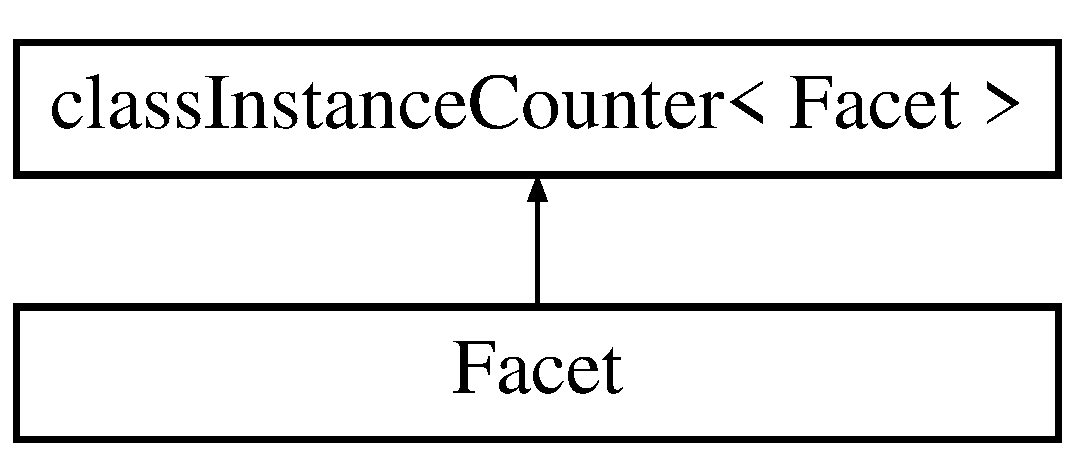
\includegraphics[height=2.000000cm]{class_facet}
\end{center}
\end{figure}
\subsection*{Public Member Functions}
\begin{DoxyCompactItemize}
\item 
\mbox{\hyperlink{class_facet_acfcdcc63ac32fc2a1d0378a899441bbc}{Facet}} (double a)
\begin{DoxyCompactList}\small\item\em Public Constructor. \end{DoxyCompactList}\item 
\mbox{\hyperlink{class_facet_aaecf4566bbdbfb3904d9c3ce6f7c41cf}{Facet}} (std\+::vector$<$ \mbox{\hyperlink{class_node}{Node}} $\ast$$>$ node\+List)
\begin{DoxyCompactList}\small\item\em Public Constructor. \end{DoxyCompactList}\item 
virtual \mbox{\hyperlink{class_facet_af40042b9ad6c5a03127034f9d1c1e786}{$\sim$\+Facet}} ()
\begin{DoxyCompactList}\small\item\em Public destructor. \end{DoxyCompactList}\item 
double \mbox{\hyperlink{class_facet_a90036d7bb3e52b57ac0d48f6bc1e019c}{get\+Area}} (void) const
\begin{DoxyCompactList}\small\item\em Query \mbox{\hyperlink{class_facet}{Facet}} object\textquotesingle{}s area. \end{DoxyCompactList}\end{DoxyCompactItemize}
\subsection*{Additional Inherited Members}


\subsection{Detailed Description}
\mbox{\hyperlink{class_facet}{Facet}} object is a triangle defined by three \mbox{\hyperlink{class_node}{Node}} objects. 

This class stores the position, defining nodes, centroid, area, other essential information, etc. for a facet element of the \mbox{\hyperlink{class_mesh}{Mesh}} object. 

\subsection{Constructor \& Destructor Documentation}
\mbox{\Hypertarget{class_facet_acfcdcc63ac32fc2a1d0378a899441bbc}\label{class_facet_acfcdcc63ac32fc2a1d0378a899441bbc}} 
\index{Facet@{Facet}!Facet@{Facet}}
\index{Facet@{Facet}!Facet@{Facet}}
\subsubsection{\texorpdfstring{Facet()}{Facet()}\hspace{0.1cm}{\footnotesize\ttfamily [1/2]}}
{\footnotesize\ttfamily Facet\+::\+Facet (\begin{DoxyParamCaption}\item[{double}]{a }\end{DoxyParamCaption})\hspace{0.3cm}{\ttfamily [inline]}}



Public Constructor. 

This constructs a \mbox{\hyperlink{class_facet}{Facet}} object with area a, under the assumption that the defining Nodes will be subsequently added. \begin{DoxyRefDesc}{Todo}
\item[\mbox{\hyperlink{todo__todo000008}{Todo}}]Need to restructure some \mbox{\hyperlink{class_mesh}{Mesh}} architecture to prevent the need for this constructor. \end{DoxyRefDesc}

\begin{DoxyParams}{Parameters}
{\em a} & {\bfseries (double)} prescribed area of the \mbox{\hyperlink{class_facet}{Facet}} to be constructed \\
\hline
\end{DoxyParams}
\begin{DoxyReturn}{Returns}
Constructed \mbox{\hyperlink{class_facet}{Facet}} object 
\end{DoxyReturn}
\mbox{\Hypertarget{class_facet_aaecf4566bbdbfb3904d9c3ce6f7c41cf}\label{class_facet_aaecf4566bbdbfb3904d9c3ce6f7c41cf}} 
\index{Facet@{Facet}!Facet@{Facet}}
\index{Facet@{Facet}!Facet@{Facet}}
\subsubsection{\texorpdfstring{Facet()}{Facet()}\hspace{0.1cm}{\footnotesize\ttfamily [2/2]}}
{\footnotesize\ttfamily Facet\+::\+Facet (\begin{DoxyParamCaption}\item[{std\+::vector$<$ \mbox{\hyperlink{class_node}{Node}} $\ast$$>$}]{node\+List }\end{DoxyParamCaption})}



Public Constructor. 

This constructs a \mbox{\hyperlink{class_facet}{Facet}} object with defining vertices given by argument node\+List \begin{DoxyRefDesc}{Todo}
\item[\mbox{\hyperlink{todo__todo000009}{Todo}}]provide checks within this constructor to either block node\+List.\+size() != 3 or generalize the \mbox{\hyperlink{class_facet}{Facet}} code to allow for arbitrary polygons as \mbox{\hyperlink{class_facet}{Facet}} objects. \end{DoxyRefDesc}

\begin{DoxyParams}{Parameters}
{\em node\+List} & {\bfseries (std\+::vector$<$\+Node$\ast$$>$)} List of \mbox{\hyperlink{class_node}{Node}} objects to use as the defining vertices for the \mbox{\hyperlink{class_facet}{Facet}} object. It is implicitly assumed here that node\+List.\+size() == 3 \\
\hline
\end{DoxyParams}
\begin{DoxyReturn}{Returns}
Constructed \mbox{\hyperlink{class_facet}{Facet}} object 
\end{DoxyReturn}
\mbox{\Hypertarget{class_facet_af40042b9ad6c5a03127034f9d1c1e786}\label{class_facet_af40042b9ad6c5a03127034f9d1c1e786}} 
\index{Facet@{Facet}!````~Facet@{$\sim$\+Facet}}
\index{````~Facet@{$\sim$\+Facet}!Facet@{Facet}}
\subsubsection{\texorpdfstring{$\sim$\+Facet()}{~Facet()}}
{\footnotesize\ttfamily virtual Facet\+::$\sim$\+Facet (\begin{DoxyParamCaption}{ }\end{DoxyParamCaption})\hspace{0.3cm}{\ttfamily [inline]}, {\ttfamily [virtual]}}



Public destructor. 

Note\+: the destructor is virtual to ensure proper decrementing of the inherited \mbox{\hyperlink{classclass_instance_counter}{class\+Instance\+Counter}} member ci\+Counter 
\begin{DoxyParams}{Parameters}
{\em None} & \\
\hline
\end{DoxyParams}
\begin{DoxyReturn}{Returns}
None 
\end{DoxyReturn}


\subsection{Member Function Documentation}
\mbox{\Hypertarget{class_facet_a90036d7bb3e52b57ac0d48f6bc1e019c}\label{class_facet_a90036d7bb3e52b57ac0d48f6bc1e019c}} 
\index{Facet@{Facet}!get\+Area@{get\+Area}}
\index{get\+Area@{get\+Area}!Facet@{Facet}}
\subsubsection{\texorpdfstring{get\+Area()}{getArea()}}
{\footnotesize\ttfamily double Facet\+::get\+Area (\begin{DoxyParamCaption}\item[{void}]{ }\end{DoxyParamCaption}) const\hspace{0.3cm}{\ttfamily [inline]}}



Query \mbox{\hyperlink{class_facet}{Facet}} object\textquotesingle{}s area. 

This function allows for public access to the \mbox{\hyperlink{class_facet}{Facet}} object\textquotesingle{}s area 
\begin{DoxyParams}{Parameters}
{\em None} & \\
\hline
\end{DoxyParams}
\begin{DoxyReturn}{Returns}
{\bfseries (double)} {\bfseries this} area property. 
\end{DoxyReturn}


The documentation for this class was generated from the following files\+:\begin{DoxyCompactItemize}
\item 
\mbox{\hyperlink{_mesh_8hpp}{Mesh.\+hpp}}\item 
\mbox{\hyperlink{_mesh_8cpp}{Mesh.\+cpp}}\end{DoxyCompactItemize}

\hypertarget{class_f_e_mesh}{}\section{F\+E\+Mesh Class Reference}
\label{class_f_e_mesh}\index{F\+E\+Mesh@{F\+E\+Mesh}}


Finite element \mbox{\hyperlink{class_mesh}{Mesh}} class.  


Inheritance diagram for F\+E\+Mesh\+:\begin{figure}[H]
\begin{center}
\leavevmode
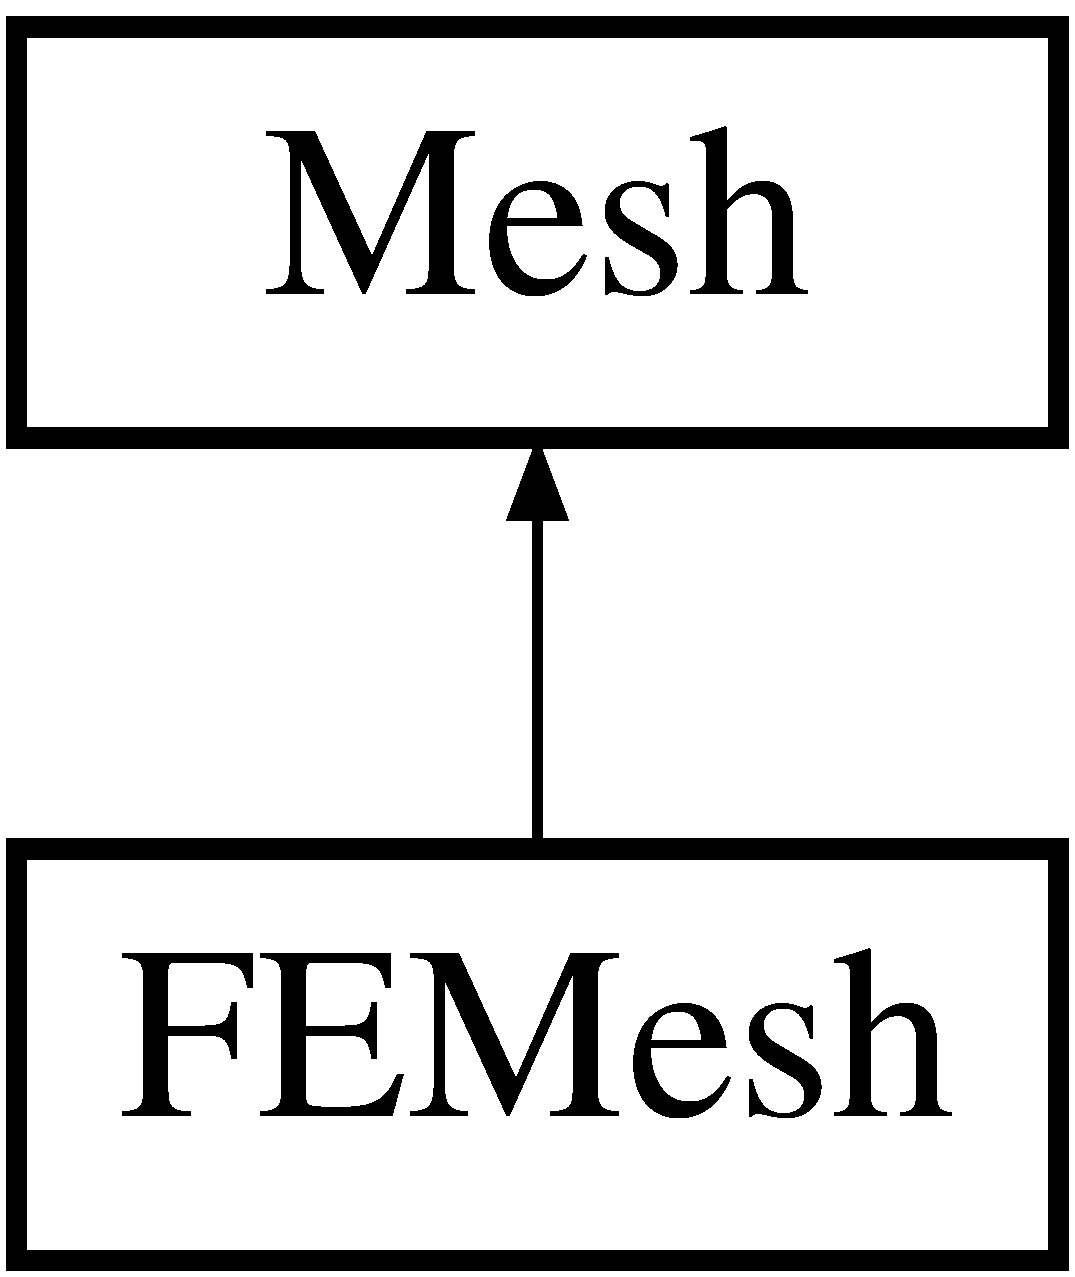
\includegraphics[height=2.000000cm]{class_f_e_mesh}
\end{center}
\end{figure}
\subsection*{Public Member Functions}
\begin{DoxyCompactItemize}
\item 
\mbox{\hyperlink{class_f_e_mesh_a3d79a6cd8810a53661cea79ed1fbe922}{F\+E\+Mesh}} (std\+::string mesh\+Data\+Filename)
\begin{DoxyCompactList}\small\item\em Public Constructor. \end{DoxyCompactList}\item 
virtual \mbox{\hyperlink{class_f_e_mesh_af4ea40d79e331fb1646da1f5766e22eb}{$\sim$\+F\+E\+Mesh}} ()
\begin{DoxyCompactList}\small\item\em Destructor. \end{DoxyCompactList}\end{DoxyCompactItemize}


\subsection{Detailed Description}
Finite element \mbox{\hyperlink{class_mesh}{Mesh}} class. 

This class, inherited from the slightly more general \mbox{\hyperlink{class_mesh}{Mesh}} class, includes the necessary components for running a finite element solver (child of \mbox{\hyperlink{class_solver_base}{Solver\+Base}}). Specifically, the \mbox{\hyperlink{class_f_e_mesh}{F\+E\+Mesh}} class includes a \mbox{\hyperlink{class_mesh}{Mesh}} object along with the associated element basis function list. 

\subsection{Constructor \& Destructor Documentation}
\mbox{\Hypertarget{class_f_e_mesh_a3d79a6cd8810a53661cea79ed1fbe922}\label{class_f_e_mesh_a3d79a6cd8810a53661cea79ed1fbe922}} 
\index{F\+E\+Mesh@{F\+E\+Mesh}!F\+E\+Mesh@{F\+E\+Mesh}}
\index{F\+E\+Mesh@{F\+E\+Mesh}!F\+E\+Mesh@{F\+E\+Mesh}}
\subsubsection{\texorpdfstring{F\+E\+Mesh()}{FEMesh()}}
{\footnotesize\ttfamily F\+E\+Mesh\+::\+F\+E\+Mesh (\begin{DoxyParamCaption}\item[{std\+::string}]{mesh\+Data\+Filename }\end{DoxyParamCaption})}



Public Constructor. 

Public constructor for \mbox{\hyperlink{class_f_e_mesh}{F\+E\+Mesh}} performs meshing of given data points, and additionally creates associated finite element basis functions \begin{DoxyRefDesc}{Todo}
\item[\mbox{\hyperlink{todo__todo000001}{Todo}}]Need to implement initialization of Basis\+El list associated with mesh \end{DoxyRefDesc}

\begin{DoxyParams}{Parameters}
{\em mesh\+Data\+Filename} & \\
\hline
\end{DoxyParams}
\begin{DoxyReturn}{Returns}
Initialized \mbox{\hyperlink{class_f_e_mesh}{F\+E\+Mesh}} object 
\end{DoxyReturn}
\mbox{\Hypertarget{class_f_e_mesh_af4ea40d79e331fb1646da1f5766e22eb}\label{class_f_e_mesh_af4ea40d79e331fb1646da1f5766e22eb}} 
\index{F\+E\+Mesh@{F\+E\+Mesh}!````~F\+E\+Mesh@{$\sim$\+F\+E\+Mesh}}
\index{````~F\+E\+Mesh@{$\sim$\+F\+E\+Mesh}!F\+E\+Mesh@{F\+E\+Mesh}}
\subsubsection{\texorpdfstring{$\sim$\+F\+E\+Mesh()}{~FEMesh()}}
{\footnotesize\ttfamily virtual F\+E\+Mesh\+::$\sim$\+F\+E\+Mesh (\begin{DoxyParamCaption}{ }\end{DoxyParamCaption})\hspace{0.3cm}{\ttfamily [inline]}, {\ttfamily [virtual]}}



Destructor. 

Note the destructor is virtual to ensure proper freeing of members if parent class delete is called 

The documentation for this class was generated from the following files\+:\begin{DoxyCompactItemize}
\item 
\mbox{\hyperlink{_f_e_mesh_8hpp}{F\+E\+Mesh.\+hpp}}\item 
\mbox{\hyperlink{_f_e_mesh_8cpp}{F\+E\+Mesh.\+cpp}}\end{DoxyCompactItemize}

\hypertarget{class_math_1_1_function}{}\section{Math\+:\+:Function Class Reference}
\label{class_math_1_1_function}\index{Math\+::\+Function@{Math\+::\+Function}}


This class associates a list of.  


Inheritance diagram for Math\+:\+:Function\+:\begin{figure}[H]
\begin{center}
\leavevmode
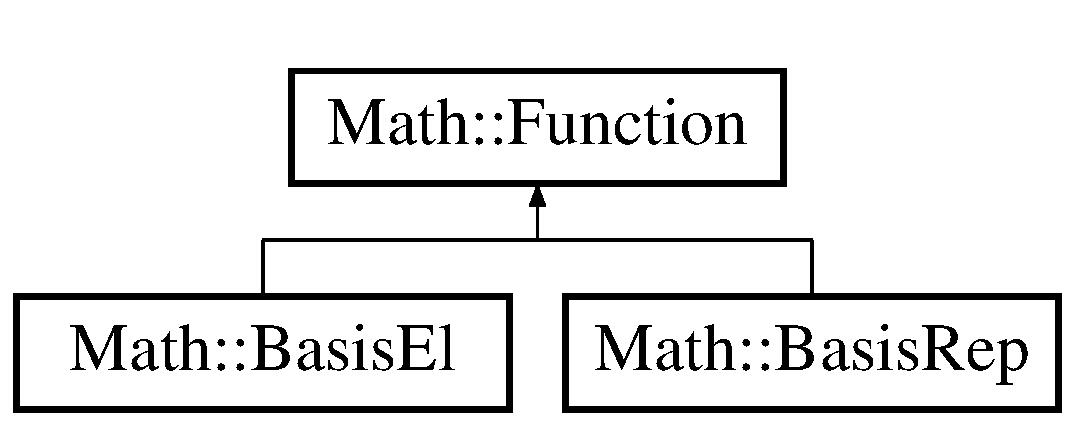
\includegraphics[height=2.000000cm]{class_math_1_1_function}
\end{center}
\end{figure}
\subsection*{Public Member Functions}
\begin{DoxyCompactItemize}
\item 
\mbox{\hyperlink{class_math_1_1_function_a97e51108b0374f8adc7982f92af4d0de}{Function}} ()
\begin{DoxyCompactList}\small\item\em Public Constructor. \end{DoxyCompactList}\item 
double \mbox{\hyperlink{class_math_1_1_function_ad85e716accc64c1ea4962c828c4e216c}{integrate\+On\+Domain}} (void)
\begin{DoxyCompactList}\small\item\em Perform integration of the function over its entire domain. \end{DoxyCompactList}\end{DoxyCompactItemize}


\subsection{Detailed Description}
This class associates a list of. 

This class implements a 2D, scalar-\/valued, piece-\/wise linear function as values associated with each \mbox{\hyperlink{class_node}{Node}} object in a given grid. The A\+PI also provides some helpful operations to be performed on the function object. 

\subsection{Constructor \& Destructor Documentation}
\mbox{\Hypertarget{class_math_1_1_function_a97e51108b0374f8adc7982f92af4d0de}\label{class_math_1_1_function_a97e51108b0374f8adc7982f92af4d0de}} 
\index{Math\+::\+Function@{Math\+::\+Function}!Function@{Function}}
\index{Function@{Function}!Math\+::\+Function@{Math\+::\+Function}}
\subsubsection{\texorpdfstring{Function()}{Function()}}
{\footnotesize\ttfamily Math\+::\+Function\+::\+Function (\begin{DoxyParamCaption}{ }\end{DoxyParamCaption})\hspace{0.3cm}{\ttfamily [inline]}}



Public Constructor. 

\begin{DoxyRefDesc}{Todo}
\item[\mbox{\hyperlink{todo__todo000003}{Todo}}]Implement a constructor with the specified parameters \end{DoxyRefDesc}

\begin{DoxyParams}{Parameters}
{\em node\+List} & {\bfseries (std\+::vector$<$\+Node$\ast$$>$)} List of 2D grid points (as \mbox{\hyperlink{class_node}{Node}} objects) on which the function object takes values \\
\hline
{\em values} & {\bfseries (std\+::vector$<$double$>$)} List of values function initially takes on each grid point. It is assumed that this list is the same size as the \mbox{\hyperlink{class_node}{Node}} list provided in first argument; optionally, if no values list is provided, all values will be initialized to zero. \\
\hline
\end{DoxyParams}
\begin{DoxyReturn}{Returns}
Initialized \mbox{\hyperlink{class_math_1_1_function}{Function}} object 
\end{DoxyReturn}


\subsection{Member Function Documentation}
\mbox{\Hypertarget{class_math_1_1_function_ad85e716accc64c1ea4962c828c4e216c}\label{class_math_1_1_function_ad85e716accc64c1ea4962c828c4e216c}} 
\index{Math\+::\+Function@{Math\+::\+Function}!integrate\+On\+Domain@{integrate\+On\+Domain}}
\index{integrate\+On\+Domain@{integrate\+On\+Domain}!Math\+::\+Function@{Math\+::\+Function}}
\subsubsection{\texorpdfstring{integrate\+On\+Domain()}{integrateOnDomain()}}
{\footnotesize\ttfamily double Math\+::\+Function\+::integrate\+On\+Domain (\begin{DoxyParamCaption}\item[{void}]{ }\end{DoxyParamCaption})}



Perform integration of the function over its entire domain. 

This method will return the definite integral of the function over the entirety of its domain. \begin{DoxyRefDesc}{Todo}
\item[\mbox{\hyperlink{todo__todo000004}{Todo}}]Method is currently not implemented \end{DoxyRefDesc}

\begin{DoxyParams}{Parameters}
{\em None} & \\
\hline
\end{DoxyParams}
\begin{DoxyReturn}{Returns}
{\bfseries (double)} value of the definite integral of the function 
\end{DoxyReturn}


The documentation for this class was generated from the following files\+:\begin{DoxyCompactItemize}
\item 
\mbox{\hyperlink{_math_8hpp}{Math.\+hpp}}\item 
\mbox{\hyperlink{_math_8cpp}{Math.\+cpp}}\end{DoxyCompactItemize}

\hypertarget{class_matrix}{}\section{Matrix Class Reference}
\label{class_matrix}\index{Matrix@{Matrix}}


Wrapper class for basic matrix operations.  


\subsection*{Public Member Functions}
\begin{DoxyCompactItemize}
\item 
\mbox{\hyperlink{class_matrix_a2dba13c45127354c9f75ef576f49269b}{Matrix}} ()
\item 
\mbox{\hyperlink{class_matrix_a4b4b9ae88079c441a7acc781fdbaa032}{Matrix}} (int \mbox{\hyperlink{class_matrix_a0eb658c64c749da9cc9705dc232fcb85}{num\+Rows}}, int \mbox{\hyperlink{class_matrix_a1ddb385f8482c80f98e5cdbf914ba11a}{num\+Cols}}=-\/1, std\+::vector$<$ double $>$ init\+Vals=\{\})
\item 
void \mbox{\hyperlink{class_matrix_a90d3e687ed2b75462f74b737d891f7ca}{Run\+Matrix\+Tests}} (void)
\item 
std\+::vector$<$ double $>$ \mbox{\hyperlink{class_matrix_ae340b61a6f3848f700ba34cd3992d2ab}{solve\+Axb}} (std\+::vector$<$ double $>$ b)
\item 
void \mbox{\hyperlink{class_matrix_a5510abd211511ab980d69b160d742f78}{rref}} (void)
\item 
std\+::vector$<$ double $>$ \mbox{\hyperlink{class_matrix_a81f93e482ceaca5d013ab34b64ee3eb4}{get\+Row}} (int row\+Num)
\item 
std\+::vector$<$ double $>$ \mbox{\hyperlink{class_matrix_a01b08c4fed1a9f7e80467e613cfc8c9e}{get\+Col}} (int col\+Num)
\item 
std\+::vector$<$ double $>$ \mbox{\hyperlink{class_matrix_adc0504b22f3d95218b5e754890f0db3e}{get\+Diag}} (void)
\item 
void \mbox{\hyperlink{class_matrix_ac9afd875262d35e1bab18604e3bc121c}{transpose}} (void)
\item 
std\+::vector$<$ double $>$ \mbox{\hyperlink{class_matrix_ac702d7055ec8bd0d804af3025b51cdec}{char\+Poly}} (void)
\item 
double \mbox{\hyperlink{class_matrix_a8229fbecb4ec1119be6c210186ecb95c}{det}} (void)
\item 
std\+::vector$<$ double $>$ \mbox{\hyperlink{class_matrix_adcb3d7e342e79b4d667860ffbf9811a1}{eig\+QR}} (double tolerance, bool verbose=false)
\item 
std\+::vector$<$ double $>$ \mbox{\hyperlink{class_matrix_a2df4b81dc518abc9fcd6896e2dafdff0}{eig\+CP}} (double tolerance, bool verbose=false)
\item 
std\+::vector$<$ double $>$ \mbox{\hyperlink{class_matrix_a107beca4305d735f074f6cb6ef97dbc9}{eig\+AI}} (double tolerance, bool verbose=false)
\item 
std\+::vector$<$ \mbox{\hyperlink{class_matrix}{Matrix}} $>$ \mbox{\hyperlink{class_matrix_ae7c92ceca24b8ca00926c93180c4cc24}{Q\+Rdecomp}} (void)
\item 
std\+::vector$<$ double $>$ \mbox{\hyperlink{class_matrix_a9fd5f24302f779d7341fdd06bb23bb90}{svd}} (double tolerance, bool verbose=false)
\item 
bool \mbox{\hyperlink{class_matrix_ae67c274d2425c1323a3a3356c174d071}{is\+Square}} (void)
\item 
\mbox{\hyperlink{class_matrix}{Matrix}} \mbox{\hyperlink{class_matrix_a0355fb02a7719e9b81938702eae3abe2}{operator=}} (const \mbox{\hyperlink{class_matrix}{Matrix}} \&rhs)
\item 
\mbox{\hyperlink{class_matrix}{Matrix}} \mbox{\hyperlink{class_matrix_ab5df6e16d56f931d712dc3b739f3e56d}{operator+}} (const \mbox{\hyperlink{class_matrix}{Matrix}} \&b)
\item 
\mbox{\hyperlink{class_matrix}{Matrix}} \mbox{\hyperlink{class_matrix_ae9f9af2349c3f6520a75116ceba73a77}{operator-\/}} (const \mbox{\hyperlink{class_matrix}{Matrix}} \&b)
\item 
\mbox{\hyperlink{class_matrix}{Matrix}} \mbox{\hyperlink{class_matrix_ac17891c37c77aabb69f2b82e15befb4d}{operator$\ast$}} (const \mbox{\hyperlink{class_matrix}{Matrix}} \&b)
\item 
std\+::vector$<$ double $>$ \mbox{\hyperlink{class_matrix_a049af5ca6904481796a79f94d8cbef31}{operator$\ast$}} (const std\+::vector$<$ double $>$ x)
\item 
bool \mbox{\hyperlink{class_matrix_a9094eaa5bbb1bdf4fb1811dfd163effb}{operator==}} (const \mbox{\hyperlink{class_matrix}{Matrix}} \&b)
\item 
double \mbox{\hyperlink{class_matrix_a0a5a42b681f5ea018e1bc6b6453b86e2}{operator\mbox{[}$\,$\mbox{]}}} (const int ij)
\item 
\mbox{\hyperlink{class_matrix}{Matrix}} \mbox{\hyperlink{class_matrix_a98b1c60f665125f2da72069314794820}{principal\+Submatrix}} (std\+::vector$<$ int $>$ ex\+Inds)
\item 
void \mbox{\hyperlink{class_matrix_a3d028bc7d149b4f87c847cf0ff50aa18}{swap\+Rows}} (int row1, int row2)
\item 
void \mbox{\hyperlink{class_matrix_a37dba2b6d455b7d44ced045ce97a9e05}{scale\+Row}} (int row, double scalar)
\item 
void \mbox{\hyperlink{class_matrix_a1385f13513c2f00cf9dbe9eb45ccbc01}{rep\+Row\+With\+Diff}} (int row1, int row2)
\item 
void \mbox{\hyperlink{class_matrix_a8e3776c15fa1abfd2ffcbd593098131f}{cat\+Row}} (std\+::vector$<$ double $>$ new\+Row)
\item 
void \mbox{\hyperlink{class_matrix_a1d288589b025eb2dad477b9699a79e9f}{cat\+Col}} (std\+::vector$<$ double $>$ new\+Col)
\item 
void \mbox{\hyperlink{class_matrix_aab389448930cfd4b32158aa58ef5f87a}{rm\+Row}} (int row\+Num)
\item 
void \mbox{\hyperlink{class_matrix_ac47f9d15d021312e0a33a341cc1e8032}{rm\+Col}} (int col\+Num)
\item 
bool \mbox{\hyperlink{class_matrix_a8001c85cc9d6a706e659f972ea35ff93}{is\+Empty}} (void)
\end{DoxyCompactItemize}
\subsection*{Public Attributes}
\begin{DoxyCompactItemize}
\item 
int \mbox{\hyperlink{class_matrix_a0eb658c64c749da9cc9705dc232fcb85}{num\+Rows}}
\item 
int \mbox{\hyperlink{class_matrix_a1ddb385f8482c80f98e5cdbf914ba11a}{num\+Cols}}
\item 
std\+::vector$<$ double $>$ \mbox{\hyperlink{class_matrix_aac8f997f1cfa7b0a0ed1d11b554a8c24}{entries}}
\end{DoxyCompactItemize}
\subsection*{Friends}
\begin{DoxyCompactItemize}
\item 
std\+::ostream \& \mbox{\hyperlink{class_matrix_ac7214274c9ef83ebef022af7225ac068}{operator$<$$<$}} (std\+::ostream \&os, const \mbox{\hyperlink{class_matrix}{Matrix}} A)
\end{DoxyCompactItemize}


\subsection{Detailed Description}
Wrapper class for basic matrix operations. 

This class stores data in a vector$<$double$>$ container, with methods intended for convenient and basic matrix operations. Currently, the \mbox{\hyperlink{class_matrix}{Matrix}} class implements relatively naive solutions to the most common linear algebra problems. Since the interface with the \mbox{\hyperlink{class_solver_base}{Solver\+Base}} classes has not yet been implemented, there is much room for refactoring here; See the associated T\+O\+DO. \begin{DoxyRefDesc}{Todo}
\item[\mbox{\hyperlink{todo__todo000006}{Todo}}]Refactor this class as a \mbox{\hyperlink{class_solver_base}{Solver\+Base}} -\/friendly wrapper for an existing linear algebra package, such as Eigen or L\+A\+P\+A\+C\+K++. \end{DoxyRefDesc}


\subsection{Constructor \& Destructor Documentation}
\mbox{\Hypertarget{class_matrix_a2dba13c45127354c9f75ef576f49269b}\label{class_matrix_a2dba13c45127354c9f75ef576f49269b}} 
\index{Matrix@{Matrix}!Matrix@{Matrix}}
\index{Matrix@{Matrix}!Matrix@{Matrix}}
\subsubsection{\texorpdfstring{Matrix()}{Matrix()}\hspace{0.1cm}{\footnotesize\ttfamily [1/2]}}
{\footnotesize\ttfamily Matrix\+::\+Matrix (\begin{DoxyParamCaption}{ }\end{DoxyParamCaption})}

\mbox{\Hypertarget{class_matrix_a4b4b9ae88079c441a7acc781fdbaa032}\label{class_matrix_a4b4b9ae88079c441a7acc781fdbaa032}} 
\index{Matrix@{Matrix}!Matrix@{Matrix}}
\index{Matrix@{Matrix}!Matrix@{Matrix}}
\subsubsection{\texorpdfstring{Matrix()}{Matrix()}\hspace{0.1cm}{\footnotesize\ttfamily [2/2]}}
{\footnotesize\ttfamily Matrix\+::\+Matrix (\begin{DoxyParamCaption}\item[{int}]{num\+Rows,  }\item[{int}]{num\+Cols = {\ttfamily -\/1},  }\item[{std\+::vector$<$ double $>$}]{init\+Vals = {\ttfamily \{\}} }\end{DoxyParamCaption})}



\subsection{Member Function Documentation}
\mbox{\Hypertarget{class_matrix_a1d288589b025eb2dad477b9699a79e9f}\label{class_matrix_a1d288589b025eb2dad477b9699a79e9f}} 
\index{Matrix@{Matrix}!cat\+Col@{cat\+Col}}
\index{cat\+Col@{cat\+Col}!Matrix@{Matrix}}
\subsubsection{\texorpdfstring{cat\+Col()}{catCol()}}
{\footnotesize\ttfamily void Matrix\+::cat\+Col (\begin{DoxyParamCaption}\item[{std\+::vector$<$ double $>$}]{new\+Col }\end{DoxyParamCaption})}

\mbox{\Hypertarget{class_matrix_a8e3776c15fa1abfd2ffcbd593098131f}\label{class_matrix_a8e3776c15fa1abfd2ffcbd593098131f}} 
\index{Matrix@{Matrix}!cat\+Row@{cat\+Row}}
\index{cat\+Row@{cat\+Row}!Matrix@{Matrix}}
\subsubsection{\texorpdfstring{cat\+Row()}{catRow()}}
{\footnotesize\ttfamily void Matrix\+::cat\+Row (\begin{DoxyParamCaption}\item[{std\+::vector$<$ double $>$}]{new\+Row }\end{DoxyParamCaption})}

\mbox{\Hypertarget{class_matrix_ac702d7055ec8bd0d804af3025b51cdec}\label{class_matrix_ac702d7055ec8bd0d804af3025b51cdec}} 
\index{Matrix@{Matrix}!char\+Poly@{char\+Poly}}
\index{char\+Poly@{char\+Poly}!Matrix@{Matrix}}
\subsubsection{\texorpdfstring{char\+Poly()}{charPoly()}}
{\footnotesize\ttfamily std\+::vector$<$ double $>$ Matrix\+::char\+Poly (\begin{DoxyParamCaption}\item[{void}]{ }\end{DoxyParamCaption})}

\mbox{\Hypertarget{class_matrix_a8229fbecb4ec1119be6c210186ecb95c}\label{class_matrix_a8229fbecb4ec1119be6c210186ecb95c}} 
\index{Matrix@{Matrix}!det@{det}}
\index{det@{det}!Matrix@{Matrix}}
\subsubsection{\texorpdfstring{det()}{det()}}
{\footnotesize\ttfamily double Matrix\+::det (\begin{DoxyParamCaption}\item[{void}]{ }\end{DoxyParamCaption})}

\mbox{\Hypertarget{class_matrix_a107beca4305d735f074f6cb6ef97dbc9}\label{class_matrix_a107beca4305d735f074f6cb6ef97dbc9}} 
\index{Matrix@{Matrix}!eig\+AI@{eig\+AI}}
\index{eig\+AI@{eig\+AI}!Matrix@{Matrix}}
\subsubsection{\texorpdfstring{eig\+A\+I()}{eigAI()}}
{\footnotesize\ttfamily std\+::vector$<$ double $>$ Matrix\+::eig\+AI (\begin{DoxyParamCaption}\item[{double}]{tolerance,  }\item[{bool}]{verbose = {\ttfamily false} }\end{DoxyParamCaption})}

\mbox{\Hypertarget{class_matrix_a2df4b81dc518abc9fcd6896e2dafdff0}\label{class_matrix_a2df4b81dc518abc9fcd6896e2dafdff0}} 
\index{Matrix@{Matrix}!eig\+CP@{eig\+CP}}
\index{eig\+CP@{eig\+CP}!Matrix@{Matrix}}
\subsubsection{\texorpdfstring{eig\+C\+P()}{eigCP()}}
{\footnotesize\ttfamily std\+::vector$<$ double $>$ Matrix\+::eig\+CP (\begin{DoxyParamCaption}\item[{double}]{tolerance,  }\item[{bool}]{verbose = {\ttfamily false} }\end{DoxyParamCaption})}

\mbox{\Hypertarget{class_matrix_adcb3d7e342e79b4d667860ffbf9811a1}\label{class_matrix_adcb3d7e342e79b4d667860ffbf9811a1}} 
\index{Matrix@{Matrix}!eig\+QR@{eig\+QR}}
\index{eig\+QR@{eig\+QR}!Matrix@{Matrix}}
\subsubsection{\texorpdfstring{eig\+Q\+R()}{eigQR()}}
{\footnotesize\ttfamily std\+::vector$<$ double $>$ Matrix\+::eig\+QR (\begin{DoxyParamCaption}\item[{double}]{tolerance,  }\item[{bool}]{verbose = {\ttfamily false} }\end{DoxyParamCaption})}

\mbox{\Hypertarget{class_matrix_a01b08c4fed1a9f7e80467e613cfc8c9e}\label{class_matrix_a01b08c4fed1a9f7e80467e613cfc8c9e}} 
\index{Matrix@{Matrix}!get\+Col@{get\+Col}}
\index{get\+Col@{get\+Col}!Matrix@{Matrix}}
\subsubsection{\texorpdfstring{get\+Col()}{getCol()}}
{\footnotesize\ttfamily std\+::vector$<$ double $>$ Matrix\+::get\+Col (\begin{DoxyParamCaption}\item[{int}]{col\+Num }\end{DoxyParamCaption})}

\mbox{\Hypertarget{class_matrix_adc0504b22f3d95218b5e754890f0db3e}\label{class_matrix_adc0504b22f3d95218b5e754890f0db3e}} 
\index{Matrix@{Matrix}!get\+Diag@{get\+Diag}}
\index{get\+Diag@{get\+Diag}!Matrix@{Matrix}}
\subsubsection{\texorpdfstring{get\+Diag()}{getDiag()}}
{\footnotesize\ttfamily std\+::vector$<$ double $>$ Matrix\+::get\+Diag (\begin{DoxyParamCaption}\item[{void}]{ }\end{DoxyParamCaption})}

\mbox{\Hypertarget{class_matrix_a81f93e482ceaca5d013ab34b64ee3eb4}\label{class_matrix_a81f93e482ceaca5d013ab34b64ee3eb4}} 
\index{Matrix@{Matrix}!get\+Row@{get\+Row}}
\index{get\+Row@{get\+Row}!Matrix@{Matrix}}
\subsubsection{\texorpdfstring{get\+Row()}{getRow()}}
{\footnotesize\ttfamily std\+::vector$<$ double $>$ Matrix\+::get\+Row (\begin{DoxyParamCaption}\item[{int}]{row\+Num }\end{DoxyParamCaption})}

\mbox{\Hypertarget{class_matrix_a8001c85cc9d6a706e659f972ea35ff93}\label{class_matrix_a8001c85cc9d6a706e659f972ea35ff93}} 
\index{Matrix@{Matrix}!is\+Empty@{is\+Empty}}
\index{is\+Empty@{is\+Empty}!Matrix@{Matrix}}
\subsubsection{\texorpdfstring{is\+Empty()}{isEmpty()}}
{\footnotesize\ttfamily bool Matrix\+::is\+Empty (\begin{DoxyParamCaption}\item[{void}]{ }\end{DoxyParamCaption})}

\mbox{\Hypertarget{class_matrix_ae67c274d2425c1323a3a3356c174d071}\label{class_matrix_ae67c274d2425c1323a3a3356c174d071}} 
\index{Matrix@{Matrix}!is\+Square@{is\+Square}}
\index{is\+Square@{is\+Square}!Matrix@{Matrix}}
\subsubsection{\texorpdfstring{is\+Square()}{isSquare()}}
{\footnotesize\ttfamily bool Matrix\+::is\+Square (\begin{DoxyParamCaption}\item[{void}]{ }\end{DoxyParamCaption})\hspace{0.3cm}{\ttfamily [inline]}}

\mbox{\Hypertarget{class_matrix_ac17891c37c77aabb69f2b82e15befb4d}\label{class_matrix_ac17891c37c77aabb69f2b82e15befb4d}} 
\index{Matrix@{Matrix}!operator$\ast$@{operator$\ast$}}
\index{operator$\ast$@{operator$\ast$}!Matrix@{Matrix}}
\subsubsection{\texorpdfstring{operator$\ast$()}{operator*()}\hspace{0.1cm}{\footnotesize\ttfamily [1/2]}}
{\footnotesize\ttfamily \mbox{\hyperlink{class_matrix}{Matrix}} Matrix\+::operator$\ast$ (\begin{DoxyParamCaption}\item[{const \mbox{\hyperlink{class_matrix}{Matrix}} \&}]{b }\end{DoxyParamCaption})}

\mbox{\Hypertarget{class_matrix_a049af5ca6904481796a79f94d8cbef31}\label{class_matrix_a049af5ca6904481796a79f94d8cbef31}} 
\index{Matrix@{Matrix}!operator$\ast$@{operator$\ast$}}
\index{operator$\ast$@{operator$\ast$}!Matrix@{Matrix}}
\subsubsection{\texorpdfstring{operator$\ast$()}{operator*()}\hspace{0.1cm}{\footnotesize\ttfamily [2/2]}}
{\footnotesize\ttfamily std\+::vector$<$ double $>$ Matrix\+::operator$\ast$ (\begin{DoxyParamCaption}\item[{const std\+::vector$<$ double $>$}]{x }\end{DoxyParamCaption})}

\mbox{\Hypertarget{class_matrix_ab5df6e16d56f931d712dc3b739f3e56d}\label{class_matrix_ab5df6e16d56f931d712dc3b739f3e56d}} 
\index{Matrix@{Matrix}!operator+@{operator+}}
\index{operator+@{operator+}!Matrix@{Matrix}}
\subsubsection{\texorpdfstring{operator+()}{operator+()}}
{\footnotesize\ttfamily \mbox{\hyperlink{class_matrix}{Matrix}} Matrix\+::operator+ (\begin{DoxyParamCaption}\item[{const \mbox{\hyperlink{class_matrix}{Matrix}} \&}]{b }\end{DoxyParamCaption})}

\mbox{\Hypertarget{class_matrix_ae9f9af2349c3f6520a75116ceba73a77}\label{class_matrix_ae9f9af2349c3f6520a75116ceba73a77}} 
\index{Matrix@{Matrix}!operator-\/@{operator-\/}}
\index{operator-\/@{operator-\/}!Matrix@{Matrix}}
\subsubsection{\texorpdfstring{operator-\/()}{operator-()}}
{\footnotesize\ttfamily \mbox{\hyperlink{class_matrix}{Matrix}} Matrix\+::operator-\/ (\begin{DoxyParamCaption}\item[{const \mbox{\hyperlink{class_matrix}{Matrix}} \&}]{b }\end{DoxyParamCaption})}

\mbox{\Hypertarget{class_matrix_a0355fb02a7719e9b81938702eae3abe2}\label{class_matrix_a0355fb02a7719e9b81938702eae3abe2}} 
\index{Matrix@{Matrix}!operator=@{operator=}}
\index{operator=@{operator=}!Matrix@{Matrix}}
\subsubsection{\texorpdfstring{operator=()}{operator=()}}
{\footnotesize\ttfamily \mbox{\hyperlink{class_matrix}{Matrix}} Matrix\+::operator= (\begin{DoxyParamCaption}\item[{const \mbox{\hyperlink{class_matrix}{Matrix}} \&}]{rhs }\end{DoxyParamCaption})}

\mbox{\Hypertarget{class_matrix_a9094eaa5bbb1bdf4fb1811dfd163effb}\label{class_matrix_a9094eaa5bbb1bdf4fb1811dfd163effb}} 
\index{Matrix@{Matrix}!operator==@{operator==}}
\index{operator==@{operator==}!Matrix@{Matrix}}
\subsubsection{\texorpdfstring{operator==()}{operator==()}}
{\footnotesize\ttfamily bool Matrix\+::operator== (\begin{DoxyParamCaption}\item[{const \mbox{\hyperlink{class_matrix}{Matrix}} \&}]{b }\end{DoxyParamCaption})}

\mbox{\Hypertarget{class_matrix_a0a5a42b681f5ea018e1bc6b6453b86e2}\label{class_matrix_a0a5a42b681f5ea018e1bc6b6453b86e2}} 
\index{Matrix@{Matrix}!operator\mbox{[}\mbox{]}@{operator[]}}
\index{operator\mbox{[}\mbox{]}@{operator[]}!Matrix@{Matrix}}
\subsubsection{\texorpdfstring{operator[]()}{operator[]()}}
{\footnotesize\ttfamily double Matrix\+::operator\mbox{[}$\,$\mbox{]} (\begin{DoxyParamCaption}\item[{const int}]{ij }\end{DoxyParamCaption})}

\mbox{\Hypertarget{class_matrix_a98b1c60f665125f2da72069314794820}\label{class_matrix_a98b1c60f665125f2da72069314794820}} 
\index{Matrix@{Matrix}!principal\+Submatrix@{principal\+Submatrix}}
\index{principal\+Submatrix@{principal\+Submatrix}!Matrix@{Matrix}}
\subsubsection{\texorpdfstring{principal\+Submatrix()}{principalSubmatrix()}}
{\footnotesize\ttfamily \mbox{\hyperlink{class_matrix}{Matrix}} Matrix\+::principal\+Submatrix (\begin{DoxyParamCaption}\item[{std\+::vector$<$ int $>$}]{ex\+Inds }\end{DoxyParamCaption})}

\mbox{\Hypertarget{class_matrix_ae7c92ceca24b8ca00926c93180c4cc24}\label{class_matrix_ae7c92ceca24b8ca00926c93180c4cc24}} 
\index{Matrix@{Matrix}!Q\+Rdecomp@{Q\+Rdecomp}}
\index{Q\+Rdecomp@{Q\+Rdecomp}!Matrix@{Matrix}}
\subsubsection{\texorpdfstring{Q\+Rdecomp()}{QRdecomp()}}
{\footnotesize\ttfamily std\+::vector$<$ \mbox{\hyperlink{class_matrix}{Matrix}} $>$ Matrix\+::\+Q\+Rdecomp (\begin{DoxyParamCaption}\item[{void}]{ }\end{DoxyParamCaption})}

\mbox{\Hypertarget{class_matrix_a1385f13513c2f00cf9dbe9eb45ccbc01}\label{class_matrix_a1385f13513c2f00cf9dbe9eb45ccbc01}} 
\index{Matrix@{Matrix}!rep\+Row\+With\+Diff@{rep\+Row\+With\+Diff}}
\index{rep\+Row\+With\+Diff@{rep\+Row\+With\+Diff}!Matrix@{Matrix}}
\subsubsection{\texorpdfstring{rep\+Row\+With\+Diff()}{repRowWithDiff()}}
{\footnotesize\ttfamily void Matrix\+::rep\+Row\+With\+Diff (\begin{DoxyParamCaption}\item[{int}]{row1,  }\item[{int}]{row2 }\end{DoxyParamCaption})}

\mbox{\Hypertarget{class_matrix_ac47f9d15d021312e0a33a341cc1e8032}\label{class_matrix_ac47f9d15d021312e0a33a341cc1e8032}} 
\index{Matrix@{Matrix}!rm\+Col@{rm\+Col}}
\index{rm\+Col@{rm\+Col}!Matrix@{Matrix}}
\subsubsection{\texorpdfstring{rm\+Col()}{rmCol()}}
{\footnotesize\ttfamily void Matrix\+::rm\+Col (\begin{DoxyParamCaption}\item[{int}]{col\+Num }\end{DoxyParamCaption})}

\mbox{\Hypertarget{class_matrix_aab389448930cfd4b32158aa58ef5f87a}\label{class_matrix_aab389448930cfd4b32158aa58ef5f87a}} 
\index{Matrix@{Matrix}!rm\+Row@{rm\+Row}}
\index{rm\+Row@{rm\+Row}!Matrix@{Matrix}}
\subsubsection{\texorpdfstring{rm\+Row()}{rmRow()}}
{\footnotesize\ttfamily void Matrix\+::rm\+Row (\begin{DoxyParamCaption}\item[{int}]{row\+Num }\end{DoxyParamCaption})}

\mbox{\Hypertarget{class_matrix_a5510abd211511ab980d69b160d742f78}\label{class_matrix_a5510abd211511ab980d69b160d742f78}} 
\index{Matrix@{Matrix}!rref@{rref}}
\index{rref@{rref}!Matrix@{Matrix}}
\subsubsection{\texorpdfstring{rref()}{rref()}}
{\footnotesize\ttfamily void Matrix\+::rref (\begin{DoxyParamCaption}\item[{void}]{ }\end{DoxyParamCaption})}

\mbox{\Hypertarget{class_matrix_a90d3e687ed2b75462f74b737d891f7ca}\label{class_matrix_a90d3e687ed2b75462f74b737d891f7ca}} 
\index{Matrix@{Matrix}!Run\+Matrix\+Tests@{Run\+Matrix\+Tests}}
\index{Run\+Matrix\+Tests@{Run\+Matrix\+Tests}!Matrix@{Matrix}}
\subsubsection{\texorpdfstring{Run\+Matrix\+Tests()}{RunMatrixTests()}}
{\footnotesize\ttfamily void Matrix\+::\+Run\+Matrix\+Tests (\begin{DoxyParamCaption}\item[{void}]{ }\end{DoxyParamCaption})}

\mbox{\Hypertarget{class_matrix_a37dba2b6d455b7d44ced045ce97a9e05}\label{class_matrix_a37dba2b6d455b7d44ced045ce97a9e05}} 
\index{Matrix@{Matrix}!scale\+Row@{scale\+Row}}
\index{scale\+Row@{scale\+Row}!Matrix@{Matrix}}
\subsubsection{\texorpdfstring{scale\+Row()}{scaleRow()}}
{\footnotesize\ttfamily void Matrix\+::scale\+Row (\begin{DoxyParamCaption}\item[{int}]{row,  }\item[{double}]{scalar }\end{DoxyParamCaption})}

\mbox{\Hypertarget{class_matrix_ae340b61a6f3848f700ba34cd3992d2ab}\label{class_matrix_ae340b61a6f3848f700ba34cd3992d2ab}} 
\index{Matrix@{Matrix}!solve\+Axb@{solve\+Axb}}
\index{solve\+Axb@{solve\+Axb}!Matrix@{Matrix}}
\subsubsection{\texorpdfstring{solve\+Axb()}{solveAxb()}}
{\footnotesize\ttfamily std\+::vector$<$ double $>$ Matrix\+::solve\+Axb (\begin{DoxyParamCaption}\item[{std\+::vector$<$ double $>$}]{b }\end{DoxyParamCaption})}

\mbox{\Hypertarget{class_matrix_a9fd5f24302f779d7341fdd06bb23bb90}\label{class_matrix_a9fd5f24302f779d7341fdd06bb23bb90}} 
\index{Matrix@{Matrix}!svd@{svd}}
\index{svd@{svd}!Matrix@{Matrix}}
\subsubsection{\texorpdfstring{svd()}{svd()}}
{\footnotesize\ttfamily std\+::vector$<$ double $>$ Matrix\+::svd (\begin{DoxyParamCaption}\item[{double}]{tolerance,  }\item[{bool}]{verbose = {\ttfamily false} }\end{DoxyParamCaption})}

\mbox{\Hypertarget{class_matrix_a3d028bc7d149b4f87c847cf0ff50aa18}\label{class_matrix_a3d028bc7d149b4f87c847cf0ff50aa18}} 
\index{Matrix@{Matrix}!swap\+Rows@{swap\+Rows}}
\index{swap\+Rows@{swap\+Rows}!Matrix@{Matrix}}
\subsubsection{\texorpdfstring{swap\+Rows()}{swapRows()}}
{\footnotesize\ttfamily void Matrix\+::swap\+Rows (\begin{DoxyParamCaption}\item[{int}]{row1,  }\item[{int}]{row2 }\end{DoxyParamCaption})}

\mbox{\Hypertarget{class_matrix_ac9afd875262d35e1bab18604e3bc121c}\label{class_matrix_ac9afd875262d35e1bab18604e3bc121c}} 
\index{Matrix@{Matrix}!transpose@{transpose}}
\index{transpose@{transpose}!Matrix@{Matrix}}
\subsubsection{\texorpdfstring{transpose()}{transpose()}}
{\footnotesize\ttfamily void Matrix\+::transpose (\begin{DoxyParamCaption}\item[{void}]{ }\end{DoxyParamCaption})}



\subsection{Friends And Related Function Documentation}
\mbox{\Hypertarget{class_matrix_ac7214274c9ef83ebef022af7225ac068}\label{class_matrix_ac7214274c9ef83ebef022af7225ac068}} 
\index{Matrix@{Matrix}!operator$<$$<$@{operator$<$$<$}}
\index{operator$<$$<$@{operator$<$$<$}!Matrix@{Matrix}}
\subsubsection{\texorpdfstring{operator$<$$<$}{operator<<}}
{\footnotesize\ttfamily std\+::ostream\& operator$<$$<$ (\begin{DoxyParamCaption}\item[{std\+::ostream \&}]{os,  }\item[{const \mbox{\hyperlink{class_matrix}{Matrix}}}]{A }\end{DoxyParamCaption})\hspace{0.3cm}{\ttfamily [friend]}}



\subsection{Member Data Documentation}
\mbox{\Hypertarget{class_matrix_aac8f997f1cfa7b0a0ed1d11b554a8c24}\label{class_matrix_aac8f997f1cfa7b0a0ed1d11b554a8c24}} 
\index{Matrix@{Matrix}!entries@{entries}}
\index{entries@{entries}!Matrix@{Matrix}}
\subsubsection{\texorpdfstring{entries}{entries}}
{\footnotesize\ttfamily std\+::vector$<$double$>$ Matrix\+::entries}

\mbox{\Hypertarget{class_matrix_a1ddb385f8482c80f98e5cdbf914ba11a}\label{class_matrix_a1ddb385f8482c80f98e5cdbf914ba11a}} 
\index{Matrix@{Matrix}!num\+Cols@{num\+Cols}}
\index{num\+Cols@{num\+Cols}!Matrix@{Matrix}}
\subsubsection{\texorpdfstring{num\+Cols}{numCols}}
{\footnotesize\ttfamily int Matrix\+::num\+Cols}

\mbox{\Hypertarget{class_matrix_a0eb658c64c749da9cc9705dc232fcb85}\label{class_matrix_a0eb658c64c749da9cc9705dc232fcb85}} 
\index{Matrix@{Matrix}!num\+Rows@{num\+Rows}}
\index{num\+Rows@{num\+Rows}!Matrix@{Matrix}}
\subsubsection{\texorpdfstring{num\+Rows}{numRows}}
{\footnotesize\ttfamily int Matrix\+::num\+Rows}



The documentation for this class was generated from the following files\+:\begin{DoxyCompactItemize}
\item 
\mbox{\hyperlink{_matrix_8hpp}{Matrix.\+hpp}}\item 
\mbox{\hyperlink{_matrix_8cpp}{Matrix.\+cpp}}\end{DoxyCompactItemize}

\hypertarget{class_mesh}{}\section{Mesh Class Reference}
\label{class_mesh}\index{Mesh@{Mesh}}


\mbox{\hyperlink{class_mesh}{Mesh}} class generates and stores a 2D mesh from an input grid points file.  


Inheritance diagram for Mesh\+:\begin{figure}[H]
\begin{center}
\leavevmode
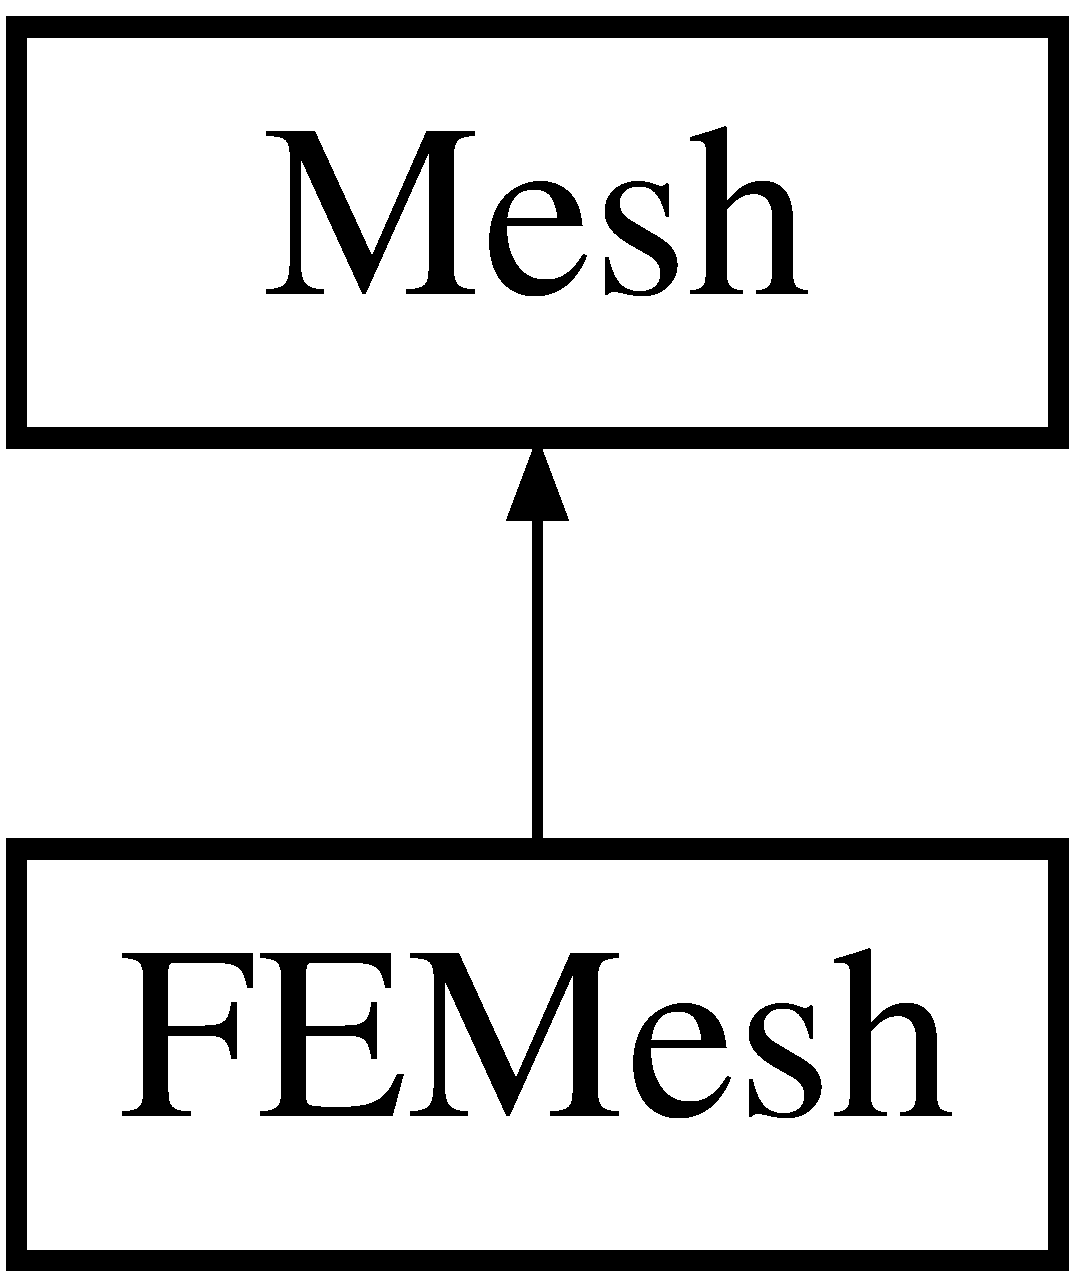
\includegraphics[height=2.000000cm]{class_mesh}
\end{center}
\end{figure}
\subsection*{Public Member Functions}
\begin{DoxyCompactItemize}
\item 
\mbox{\hyperlink{class_mesh_ade26657ad48e8e84af8a2614a8ac6b0c}{Mesh}} (std\+::string mesh\+Data\+Filename, bool rot\+Flag=false)
\begin{DoxyCompactList}\small\item\em Public Constructor. \end{DoxyCompactList}\item 
\mbox{\hyperlink{class_mesh_a5efe4da1a4c0971cfb037bd70304c303}{$\sim$\+Mesh}} ()
\begin{DoxyCompactList}\small\item\em Destructor. \end{DoxyCompactList}\item 
void \mbox{\hyperlink{class_mesh_a4d194fe4ce2b4fa4c11274c893c6ae29}{write\+Mesh}} (std\+::string mesh\+Out\+File=\char`\"{}Mesh.\+out\char`\"{})
\begin{DoxyCompactList}\small\item\em Writes relevant mesh data to the provided output file name. \end{DoxyCompactList}\item 
unsigned \mbox{\hyperlink{class_mesh_a716f8cde80ac5f0ed592aaa56995f618}{size}} (void) const
\begin{DoxyCompactList}\small\item\em Query the size of the mesh (equivalently, number of nodes in mesh/grid) \end{DoxyCompactList}\item 
\mbox{\hyperlink{class_mesh}{Mesh}} \mbox{\hyperlink{class_mesh_a732e258583e090537f7c47b9a7594e85}{operator=}} (const \mbox{\hyperlink{class_mesh}{Mesh}} \&rhs)
\begin{DoxyCompactList}\small\item\em Assignment operator. \end{DoxyCompactList}\item 
const \mbox{\hyperlink{class_node}{Node}} $\ast$ \mbox{\hyperlink{class_mesh_afbb98e084a07e94b5d3ad503aaa82e08}{nodelist}} (size\+\_\+t i) const
\begin{DoxyCompactList}\small\item\em Returns (as read-\/only) the i-\/th node in the \mbox{\hyperlink{class_mesh}{Mesh}} objects node list. \end{DoxyCompactList}\end{DoxyCompactItemize}


\subsection{Detailed Description}
\mbox{\hyperlink{class_mesh}{Mesh}} class generates and stores a 2D mesh from an input grid points file. 

This class generates and stores a 2D mesh from an input grid points file. A divide-\/and-\/conquer {\bfseries \href{https://en.wikipedia.org/wiki/Delaunay_triangulation}{\tt Delaunay Triangulation}} algorithm is implemented and requires as input a 2D grid point file. The class generates the list of nodes/adjacencies with the facet objects that are used in the finite element solver classes. \begin{DoxyRefDesc}{Todo}
\item[\mbox{\hyperlink{todo__todo000007}{Todo}}]Allow for constrained DT \end{DoxyRefDesc}


\subsection{Constructor \& Destructor Documentation}
\mbox{\Hypertarget{class_mesh_ade26657ad48e8e84af8a2614a8ac6b0c}\label{class_mesh_ade26657ad48e8e84af8a2614a8ac6b0c}} 
\index{Mesh@{Mesh}!Mesh@{Mesh}}
\index{Mesh@{Mesh}!Mesh@{Mesh}}
\subsubsection{\texorpdfstring{Mesh()}{Mesh()}}
{\footnotesize\ttfamily Mesh\+::\+Mesh (\begin{DoxyParamCaption}\item[{std\+::string}]{mesh\+Data\+Filename,  }\item[{bool}]{rot\+Flag = {\ttfamily false} }\end{DoxyParamCaption})}



Public Constructor. 

This public constructor parses the provided grid point file and performs the triangulation, constructing the node and facet list required 
\begin{DoxyParams}{Parameters}
{\em mesh\+Data\+Filename} & {\bfseries (std\+::string)} The grid point data file name to be parsed for grid point locations \\
\hline
{\em rot\+Flag} & {\bfseries (bool)} whether to linearly rotate the grid points prior to meshing (and rotate back after meshing) \\
\hline
\end{DoxyParams}
\begin{DoxyReturn}{Returns}
Constructed \mbox{\hyperlink{class_mesh}{Mesh}} object 
\end{DoxyReturn}
\mbox{\Hypertarget{class_mesh_a5efe4da1a4c0971cfb037bd70304c303}\label{class_mesh_a5efe4da1a4c0971cfb037bd70304c303}} 
\index{Mesh@{Mesh}!````~Mesh@{$\sim$\+Mesh}}
\index{````~Mesh@{$\sim$\+Mesh}!Mesh@{Mesh}}
\subsubsection{\texorpdfstring{$\sim$\+Mesh()}{~Mesh()}}
{\footnotesize\ttfamily Mesh\+::$\sim$\+Mesh (\begin{DoxyParamCaption}{ }\end{DoxyParamCaption})}



Destructor. 

Performs necessary gargbage clean-\/up (frees node/facet list members) 
\begin{DoxyParams}{Parameters}
{\em None} & \\
\hline
\end{DoxyParams}
\begin{DoxyReturn}{Returns}
None 
\end{DoxyReturn}


\subsection{Member Function Documentation}
\mbox{\Hypertarget{class_mesh_afbb98e084a07e94b5d3ad503aaa82e08}\label{class_mesh_afbb98e084a07e94b5d3ad503aaa82e08}} 
\index{Mesh@{Mesh}!nodelist@{nodelist}}
\index{nodelist@{nodelist}!Mesh@{Mesh}}
\subsubsection{\texorpdfstring{nodelist()}{nodelist()}}
{\footnotesize\ttfamily const \mbox{\hyperlink{class_node}{Node}} $\ast$ Mesh\+::nodelist (\begin{DoxyParamCaption}\item[{size\+\_\+t}]{i }\end{DoxyParamCaption}) const}



Returns (as read-\/only) the i-\/th node in the \mbox{\hyperlink{class_mesh}{Mesh}} objects node list. 

Note\+: this function performs an i $<$ {\bfseries this}-\/$>$nodelist.\+size() ? check to guard against invalid accesses. A runtime error is thrown if i $>$= {\bfseries this}-\/$>$node\+List.\+size() 
\begin{DoxyParams}{Parameters}
{\em i} & {\bfseries (size\+\_\+t)} index of node in node list to access \\
\hline
\end{DoxyParams}
\begin{DoxyReturn}{Returns}
{\bfseries (const Node$\ast$)} \mbox{\hyperlink{class_node}{Node}} object at index i in {\bfseries this}-\/$>$node\+List 
\end{DoxyReturn}
\mbox{\Hypertarget{class_mesh_a732e258583e090537f7c47b9a7594e85}\label{class_mesh_a732e258583e090537f7c47b9a7594e85}} 
\index{Mesh@{Mesh}!operator=@{operator=}}
\index{operator=@{operator=}!Mesh@{Mesh}}
\subsubsection{\texorpdfstring{operator=()}{operator=()}}
{\footnotesize\ttfamily \mbox{\hyperlink{class_mesh}{Mesh}} Mesh\+::operator= (\begin{DoxyParamCaption}\item[{const \mbox{\hyperlink{class_mesh}{Mesh}} \&}]{rhs }\end{DoxyParamCaption})}



Assignment operator. 

This operator performs a copy assignment to the left-\/hand side \mbox{\hyperlink{class_mesh}{Mesh}} object 
\begin{DoxyParams}{Parameters}
{\em rhs} & {\bfseries (\mbox{\hyperlink{class_mesh}{Mesh}})} the \mbox{\hyperlink{class_mesh}{Mesh}} object to be copied left \\
\hline
\end{DoxyParams}
\begin{DoxyReturn}{Returns}
{\bfseries (\mbox{\hyperlink{class_mesh}{Mesh}})} the left-\/hand side \mbox{\hyperlink{class_mesh}{Mesh}} object, with data members set to rhs\textquotesingle{} 
\end{DoxyReturn}
\mbox{\Hypertarget{class_mesh_a716f8cde80ac5f0ed592aaa56995f618}\label{class_mesh_a716f8cde80ac5f0ed592aaa56995f618}} 
\index{Mesh@{Mesh}!size@{size}}
\index{size@{size}!Mesh@{Mesh}}
\subsubsection{\texorpdfstring{size()}{size()}}
{\footnotesize\ttfamily unsigned Mesh\+::size (\begin{DoxyParamCaption}\item[{void}]{ }\end{DoxyParamCaption}) const\hspace{0.3cm}{\ttfamily [inline]}}



Query the size of the mesh (equivalently, number of nodes in mesh/grid) 

Note\+: this size may significantly differ from the number of facet in the \mbox{\hyperlink{class_mesh}{Mesh}} object 
\begin{DoxyParams}{Parameters}
{\em None} & \\
\hline
\end{DoxyParams}
\begin{DoxyReturn}{Returns}
{\bfseries (unsigned)} size of the \mbox{\hyperlink{class_mesh}{Mesh}} object (number of nodes in the \mbox{\hyperlink{class_mesh}{Mesh}}) 
\end{DoxyReturn}
\mbox{\Hypertarget{class_mesh_a4d194fe4ce2b4fa4c11274c893c6ae29}\label{class_mesh_a4d194fe4ce2b4fa4c11274c893c6ae29}} 
\index{Mesh@{Mesh}!write\+Mesh@{write\+Mesh}}
\index{write\+Mesh@{write\+Mesh}!Mesh@{Mesh}}
\subsubsection{\texorpdfstring{write\+Mesh()}{writeMesh()}}
{\footnotesize\ttfamily void Mesh\+::write\+Mesh (\begin{DoxyParamCaption}\item[{std\+::string}]{mesh\+Out\+File = {\ttfamily \char`\"{}Mesh.out\char`\"{}} }\end{DoxyParamCaption})}



Writes relevant mesh data to the provided output file name. 

This function writes all data to the provided output file necessary to exactly reconstruct the computed mesh. 
\begin{DoxyParams}{Parameters}
{\em mesh\+Out\+File} & {\bfseries (std\+::string)} file name of output file in which to write the computed mesh data \\
\hline
\end{DoxyParams}
\begin{DoxyReturn}{Returns}
None 
\end{DoxyReturn}


The documentation for this class was generated from the following files\+:\begin{DoxyCompactItemize}
\item 
\mbox{\hyperlink{_mesh_8hpp}{Mesh.\+hpp}}\item 
\mbox{\hyperlink{_mesh_8cpp}{Mesh.\+cpp}}\end{DoxyCompactItemize}

\hypertarget{class_node}{}\section{Node Class Reference}
\label{class_node}\index{Node@{Node}}


\mbox{\hyperlink{class_node}{Node}} class provides A\+PI for a vertex object in a \mbox{\hyperlink{class_mesh}{Mesh}}.  


Inheritance diagram for Node\+:\begin{figure}[H]
\begin{center}
\leavevmode
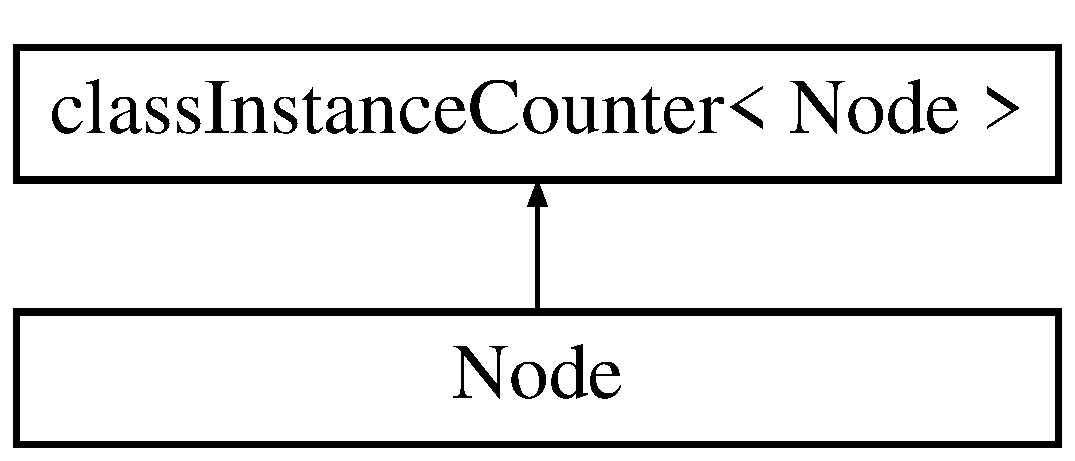
\includegraphics[height=2.000000cm]{class_node}
\end{center}
\end{figure}
\subsection*{Public Member Functions}
\begin{DoxyCompactItemize}
\item 
\mbox{\hyperlink{class_node_a75560296eb48863988f31c8adf370dcf}{Node}} (int ID, double \mbox{\hyperlink{class_node_a05d427a6fef833a49306b2adb52ef722}{x}}, double \mbox{\hyperlink{class_node_a5a06c0e486aa39a994b6a2fa674aa493}{y}})
\begin{DoxyCompactList}\small\item\em Public Constructor. \end{DoxyCompactList}\item 
virtual \mbox{\hyperlink{class_node_aa0840c3cb5c7159be6d992adecd2097c}{$\sim$\+Node}} ()
\begin{DoxyCompactList}\small\item\em Public destructor. \end{DoxyCompactList}\item 
bool \mbox{\hyperlink{class_node_aeda47a1decedb8fc3835579d75b7d65f}{operator$<$}} (\mbox{\hyperlink{class_node}{Node}} \&rhs) const
\begin{DoxyCompactList}\small\item\em Less than operator. \end{DoxyCompactList}\item 
std\+::vector$<$ double $>$ \mbox{\hyperlink{class_node_ae59cc8d62b6cfa623252b98341c3084c}{get\+Loc}} (void) const
\begin{DoxyCompactList}\small\item\em Query 2D location of \mbox{\hyperlink{class_node}{Node}} object. \end{DoxyCompactList}\item 
double \mbox{\hyperlink{class_node_a05d427a6fef833a49306b2adb52ef722}{x}} (void) const
\begin{DoxyCompactList}\small\item\em Query abscissa value location of \mbox{\hyperlink{class_node}{Node}} object. \end{DoxyCompactList}\item 
double \mbox{\hyperlink{class_node_a5a06c0e486aa39a994b6a2fa674aa493}{y}} (void) const
\begin{DoxyCompactList}\small\item\em Query ordinate value location of \mbox{\hyperlink{class_node}{Node}} object. \end{DoxyCompactList}\end{DoxyCompactItemize}
\subsection*{Additional Inherited Members}


\subsection{Detailed Description}
\mbox{\hyperlink{class_node}{Node}} class provides A\+PI for a vertex object in a \mbox{\hyperlink{class_mesh}{Mesh}}. 

This class stores the (2D) location and adjacency information for each point (i.\+e., \mbox{\hyperlink{class_node}{Node}}) in the \mbox{\hyperlink{class_mesh}{Mesh}} object. It also provides (through a private A\+PI to it\textquotesingle{}s friend class \mbox{\hyperlink{class_mesh}{Mesh}}) the necessary computations (relative to {\bfseries this}) for computing the Delaunay triangulation performed in the \mbox{\hyperlink{class_mesh}{Mesh}} constructor. 

\subsection{Constructor \& Destructor Documentation}
\mbox{\Hypertarget{class_node_a75560296eb48863988f31c8adf370dcf}\label{class_node_a75560296eb48863988f31c8adf370dcf}} 
\index{Node@{Node}!Node@{Node}}
\index{Node@{Node}!Node@{Node}}
\subsubsection{\texorpdfstring{Node()}{Node()}}
{\footnotesize\ttfamily Node\+::\+Node (\begin{DoxyParamCaption}\item[{int}]{ID,  }\item[{double}]{x,  }\item[{double}]{y }\end{DoxyParamCaption})}



Public Constructor. 

This public constructor initialized the \mbox{\hyperlink{class_node}{Node}} object\textquotesingle{}s location and ID (used for bookkeeping) 
\begin{DoxyParams}{Parameters}
{\em ID} & {\bfseries (int)} identification number used for bookkeeping in \mbox{\hyperlink{class_mesh}{Mesh}} class \\
\hline
{\em x} & {\bfseries (double)} abscissa value of \mbox{\hyperlink{class_node}{Node}} object in 2D coordinate system \\
\hline
{\em y} & {\bfseries (double)} ordinate value of \mbox{\hyperlink{class_node}{Node}} object in 2D coordinate system \\
\hline
\end{DoxyParams}
\begin{DoxyReturn}{Returns}
Constructed \mbox{\hyperlink{class_node}{Node}} object 
\end{DoxyReturn}
\mbox{\Hypertarget{class_node_aa0840c3cb5c7159be6d992adecd2097c}\label{class_node_aa0840c3cb5c7159be6d992adecd2097c}} 
\index{Node@{Node}!````~Node@{$\sim$\+Node}}
\index{````~Node@{$\sim$\+Node}!Node@{Node}}
\subsubsection{\texorpdfstring{$\sim$\+Node()}{~Node()}}
{\footnotesize\ttfamily Node\+::$\sim$\+Node (\begin{DoxyParamCaption}{ }\end{DoxyParamCaption})\hspace{0.3cm}{\ttfamily [virtual]}}



Public destructor. 

Note\+: the destructor is virtual to ensure proper decrementing of the inherited \mbox{\hyperlink{classclass_instance_counter}{class\+Instance\+Counter}} member ci\+Counter 
\begin{DoxyParams}{Parameters}
{\em None} & \\
\hline
\end{DoxyParams}
\begin{DoxyReturn}{Returns}
None 
\end{DoxyReturn}


\subsection{Member Function Documentation}
\mbox{\Hypertarget{class_node_ae59cc8d62b6cfa623252b98341c3084c}\label{class_node_ae59cc8d62b6cfa623252b98341c3084c}} 
\index{Node@{Node}!get\+Loc@{get\+Loc}}
\index{get\+Loc@{get\+Loc}!Node@{Node}}
\subsubsection{\texorpdfstring{get\+Loc()}{getLoc()}}
{\footnotesize\ttfamily std\+::vector$<$double$>$ Node\+::get\+Loc (\begin{DoxyParamCaption}\item[{void}]{ }\end{DoxyParamCaption}) const\hspace{0.3cm}{\ttfamily [inline]}}



Query 2D location of \mbox{\hyperlink{class_node}{Node}} object. 


\begin{DoxyParams}{Parameters}
{\em None} & \\
\hline
\end{DoxyParams}
\begin{DoxyReturn}{Returns}
{\bfseries (std\+::vector$<$int$>$)} 2D coordinate system location of \mbox{\hyperlink{class_node}{Node}} object 
\end{DoxyReturn}
\mbox{\Hypertarget{class_node_aeda47a1decedb8fc3835579d75b7d65f}\label{class_node_aeda47a1decedb8fc3835579d75b7d65f}} 
\index{Node@{Node}!operator$<$@{operator$<$}}
\index{operator$<$@{operator$<$}!Node@{Node}}
\subsubsection{\texorpdfstring{operator$<$()}{operator<()}}
{\footnotesize\ttfamily bool Node\+::operator$<$ (\begin{DoxyParamCaption}\item[{\mbox{\hyperlink{class_node}{Node}} \&}]{rhs }\end{DoxyParamCaption}) const}



Less than operator. 

This less than operator implements a dictionary order on the 2D coordinate location of {\bfseries this} relative to rhs 
\begin{DoxyParams}{Parameters}
{\em rhs} & {\bfseries (\mbox{\hyperlink{class_node}{Node}})} right-\/hand side of less-\/than operator (\mbox{\hyperlink{class_node}{Node}} to be compared with {\bfseries this}) \\
\hline
\end{DoxyParams}
\begin{DoxyReturn}{Returns}
{\bfseries (bool)} The dictionary order of ({\bfseries this}-\/$>$x,{\bfseries this}-\/$>$y) with (rhs-\/$>$x,rhs-\/$>$y) 
\end{DoxyReturn}
\mbox{\Hypertarget{class_node_a05d427a6fef833a49306b2adb52ef722}\label{class_node_a05d427a6fef833a49306b2adb52ef722}} 
\index{Node@{Node}!x@{x}}
\index{x@{x}!Node@{Node}}
\subsubsection{\texorpdfstring{x()}{x()}}
{\footnotesize\ttfamily double Node\+::x (\begin{DoxyParamCaption}\item[{void}]{ }\end{DoxyParamCaption}) const\hspace{0.3cm}{\ttfamily [inline]}}



Query abscissa value location of \mbox{\hyperlink{class_node}{Node}} object. 


\begin{DoxyParams}{Parameters}
{\em None} & \\
\hline
\end{DoxyParams}
\begin{DoxyReturn}{Returns}
{\bfseries (double)} {\bfseries this} abscissa value 
\end{DoxyReturn}
\mbox{\Hypertarget{class_node_a5a06c0e486aa39a994b6a2fa674aa493}\label{class_node_a5a06c0e486aa39a994b6a2fa674aa493}} 
\index{Node@{Node}!y@{y}}
\index{y@{y}!Node@{Node}}
\subsubsection{\texorpdfstring{y()}{y()}}
{\footnotesize\ttfamily double Node\+::y (\begin{DoxyParamCaption}\item[{void}]{ }\end{DoxyParamCaption}) const\hspace{0.3cm}{\ttfamily [inline]}}



Query ordinate value location of \mbox{\hyperlink{class_node}{Node}} object. 


\begin{DoxyParams}{Parameters}
{\em None} & \\
\hline
\end{DoxyParams}
\begin{DoxyReturn}{Returns}
{\bfseries (double)} {\bfseries this} ordinate value 
\end{DoxyReturn}


The documentation for this class was generated from the following files\+:\begin{DoxyCompactItemize}
\item 
\mbox{\hyperlink{_mesh_8hpp}{Mesh.\+hpp}}\item 
\mbox{\hyperlink{_mesh_8cpp}{Mesh.\+cpp}}\end{DoxyCompactItemize}

\hypertarget{class_options}{}\section{Options Class Reference}
\label{class_options}\index{Options@{Options}}
\subsection*{Public Member Functions}
\begin{DoxyCompactItemize}
\item 
\mbox{\hyperlink{class_options_af65f2f452a673db877590dbff53115ff}{Options}} (int argc, const char $\ast$argv\mbox{[}$\,$\mbox{]})
\item 
\mbox{\hyperlink{class_options_a86ddb85b183f8b58af5481f30a42fa92}{$\sim$\+Options}} ()
\item 
std\+::string \mbox{\hyperlink{class_options_af5fc0ecb4b117c5438f07762fa7f565a}{infile}} (void) const
\item 
std\+::string \mbox{\hyperlink{class_options_a35e8029289fef81902b98422e5b9aff8}{outfile}} (void) const
\item 
bool \mbox{\hyperlink{class_options_a6d00df300abbec9c39990eb8858f1255}{plot}} (void)
\item 
bool \mbox{\hyperlink{class_options_a896737c665d9c0ee7a17a0cdedf66bb7}{rotflag}} (void)
\end{DoxyCompactItemize}
\subsection*{Public Attributes}
\begin{DoxyCompactItemize}
\item 
bool \mbox{\hyperlink{class_options_a762a0775c9b60ceb2737dc90c96f7c0b}{run}}
\end{DoxyCompactItemize}


\subsection{Constructor \& Destructor Documentation}
\mbox{\Hypertarget{class_options_af65f2f452a673db877590dbff53115ff}\label{class_options_af65f2f452a673db877590dbff53115ff}} 
\index{Options@{Options}!Options@{Options}}
\index{Options@{Options}!Options@{Options}}
\subsubsection{\texorpdfstring{Options()}{Options()}}
{\footnotesize\ttfamily Options\+::\+Options (\begin{DoxyParamCaption}\item[{int}]{argc,  }\item[{const char $\ast$}]{argv\mbox{[}$\,$\mbox{]} }\end{DoxyParamCaption})}

\mbox{\Hypertarget{class_options_a86ddb85b183f8b58af5481f30a42fa92}\label{class_options_a86ddb85b183f8b58af5481f30a42fa92}} 
\index{Options@{Options}!````~Options@{$\sim$\+Options}}
\index{````~Options@{$\sim$\+Options}!Options@{Options}}
\subsubsection{\texorpdfstring{$\sim$\+Options()}{~Options()}}
{\footnotesize\ttfamily Options\+::$\sim$\+Options (\begin{DoxyParamCaption}{ }\end{DoxyParamCaption})}



\subsection{Member Function Documentation}
\mbox{\Hypertarget{class_options_af5fc0ecb4b117c5438f07762fa7f565a}\label{class_options_af5fc0ecb4b117c5438f07762fa7f565a}} 
\index{Options@{Options}!infile@{infile}}
\index{infile@{infile}!Options@{Options}}
\subsubsection{\texorpdfstring{infile()}{infile()}}
{\footnotesize\ttfamily std\+::string Options\+::infile (\begin{DoxyParamCaption}\item[{void}]{ }\end{DoxyParamCaption}) const\hspace{0.3cm}{\ttfamily [inline]}}

\mbox{\Hypertarget{class_options_a35e8029289fef81902b98422e5b9aff8}\label{class_options_a35e8029289fef81902b98422e5b9aff8}} 
\index{Options@{Options}!outfile@{outfile}}
\index{outfile@{outfile}!Options@{Options}}
\subsubsection{\texorpdfstring{outfile()}{outfile()}}
{\footnotesize\ttfamily std\+::string Options\+::outfile (\begin{DoxyParamCaption}\item[{void}]{ }\end{DoxyParamCaption}) const\hspace{0.3cm}{\ttfamily [inline]}}

\mbox{\Hypertarget{class_options_a6d00df300abbec9c39990eb8858f1255}\label{class_options_a6d00df300abbec9c39990eb8858f1255}} 
\index{Options@{Options}!plot@{plot}}
\index{plot@{plot}!Options@{Options}}
\subsubsection{\texorpdfstring{plot()}{plot()}}
{\footnotesize\ttfamily bool Options\+::plot (\begin{DoxyParamCaption}\item[{void}]{ }\end{DoxyParamCaption})\hspace{0.3cm}{\ttfamily [inline]}}

\mbox{\Hypertarget{class_options_a896737c665d9c0ee7a17a0cdedf66bb7}\label{class_options_a896737c665d9c0ee7a17a0cdedf66bb7}} 
\index{Options@{Options}!rotflag@{rotflag}}
\index{rotflag@{rotflag}!Options@{Options}}
\subsubsection{\texorpdfstring{rotflag()}{rotflag()}}
{\footnotesize\ttfamily bool Options\+::rotflag (\begin{DoxyParamCaption}\item[{void}]{ }\end{DoxyParamCaption})\hspace{0.3cm}{\ttfamily [inline]}}



\subsection{Member Data Documentation}
\mbox{\Hypertarget{class_options_a762a0775c9b60ceb2737dc90c96f7c0b}\label{class_options_a762a0775c9b60ceb2737dc90c96f7c0b}} 
\index{Options@{Options}!run@{run}}
\index{run@{run}!Options@{Options}}
\subsubsection{\texorpdfstring{run}{run}}
{\footnotesize\ttfamily bool Options\+::run}



The documentation for this class was generated from the following files\+:\begin{DoxyCompactItemize}
\item 
\mbox{\hyperlink{_options_8hpp}{Options.\+hpp}}\item 
\mbox{\hyperlink{_options_8cpp}{Options.\+cpp}}\end{DoxyCompactItemize}

\hypertarget{class_solver_base}{}\section{Solver\+Base Class Reference}
\label{class_solver_base}\index{Solver\+Base@{Solver\+Base}}
Inheritance diagram for Solver\+Base\+:\begin{figure}[H]
\begin{center}
\leavevmode
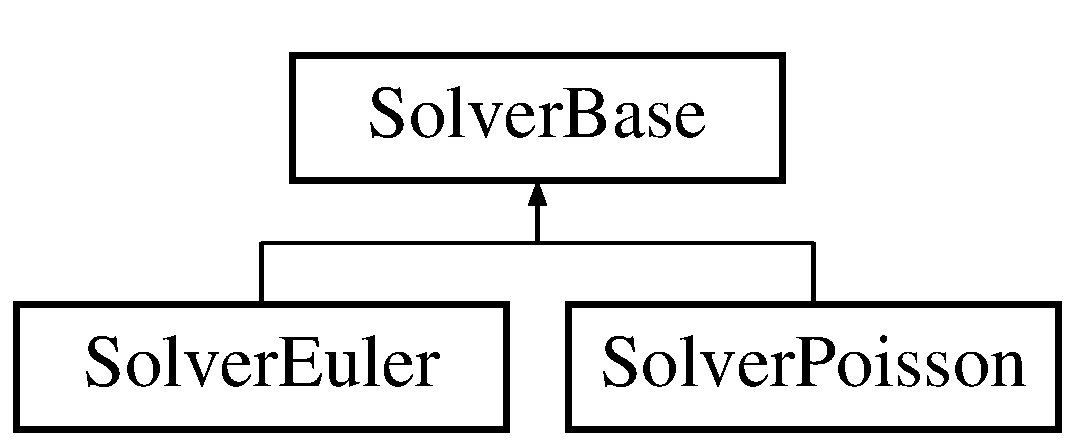
\includegraphics[height=2.000000cm]{class_solver_base}
\end{center}
\end{figure}
\subsection*{Public Member Functions}
\begin{DoxyCompactItemize}
\item 
\mbox{\hyperlink{class_solver_base_a378bd67662e76348c3ef38edd312b5e1}{Solver\+Base}} (const \mbox{\hyperlink{class_mesh}{Mesh}} $\ast$mesh)
\item 
virtual void \mbox{\hyperlink{class_solver_base_a14b5e9482f698d36dff3b43d3a4f05f1}{integrate\+In\+Time}} (double current\+Time, double dt)=0
\end{DoxyCompactItemize}


\subsection{Constructor \& Destructor Documentation}
\mbox{\Hypertarget{class_solver_base_a378bd67662e76348c3ef38edd312b5e1}\label{class_solver_base_a378bd67662e76348c3ef38edd312b5e1}} 
\index{Solver\+Base@{Solver\+Base}!Solver\+Base@{Solver\+Base}}
\index{Solver\+Base@{Solver\+Base}!Solver\+Base@{Solver\+Base}}
\subsubsection{\texorpdfstring{Solver\+Base()}{SolverBase()}}
{\footnotesize\ttfamily Solver\+Base\+::\+Solver\+Base (\begin{DoxyParamCaption}\item[{const \mbox{\hyperlink{class_mesh}{Mesh}} $\ast$}]{mesh }\end{DoxyParamCaption})}



\subsection{Member Function Documentation}
\mbox{\Hypertarget{class_solver_base_a14b5e9482f698d36dff3b43d3a4f05f1}\label{class_solver_base_a14b5e9482f698d36dff3b43d3a4f05f1}} 
\index{Solver\+Base@{Solver\+Base}!integrate\+In\+Time@{integrate\+In\+Time}}
\index{integrate\+In\+Time@{integrate\+In\+Time}!Solver\+Base@{Solver\+Base}}
\subsubsection{\texorpdfstring{integrate\+In\+Time()}{integrateInTime()}}
{\footnotesize\ttfamily virtual void Solver\+Base\+::integrate\+In\+Time (\begin{DoxyParamCaption}\item[{double}]{current\+Time,  }\item[{double}]{dt }\end{DoxyParamCaption})\hspace{0.3cm}{\ttfamily [pure virtual]}}



Implemented in \mbox{\hyperlink{class_solver_euler_a64caa7276a35f9e5408bec75bc2d3189}{Solver\+Euler}}.



The documentation for this class was generated from the following files\+:\begin{DoxyCompactItemize}
\item 
\mbox{\hyperlink{_solver_8hpp}{Solver.\+hpp}}\item 
\mbox{\hyperlink{_solver_8cpp}{Solver.\+cpp}}\end{DoxyCompactItemize}

\hypertarget{class_solver_euler}{}\section{Solver\+Euler Class Reference}
\label{class_solver_euler}\index{Solver\+Euler@{Solver\+Euler}}


Class for implementing compressible Euler equations on provided finite element mesh. See \mbox{\hyperlink{class_solver_base}{Solver\+Base}} for boundary conditions specifications.  


Inheritance diagram for Solver\+Euler\+:\begin{figure}[H]
\begin{center}
\leavevmode
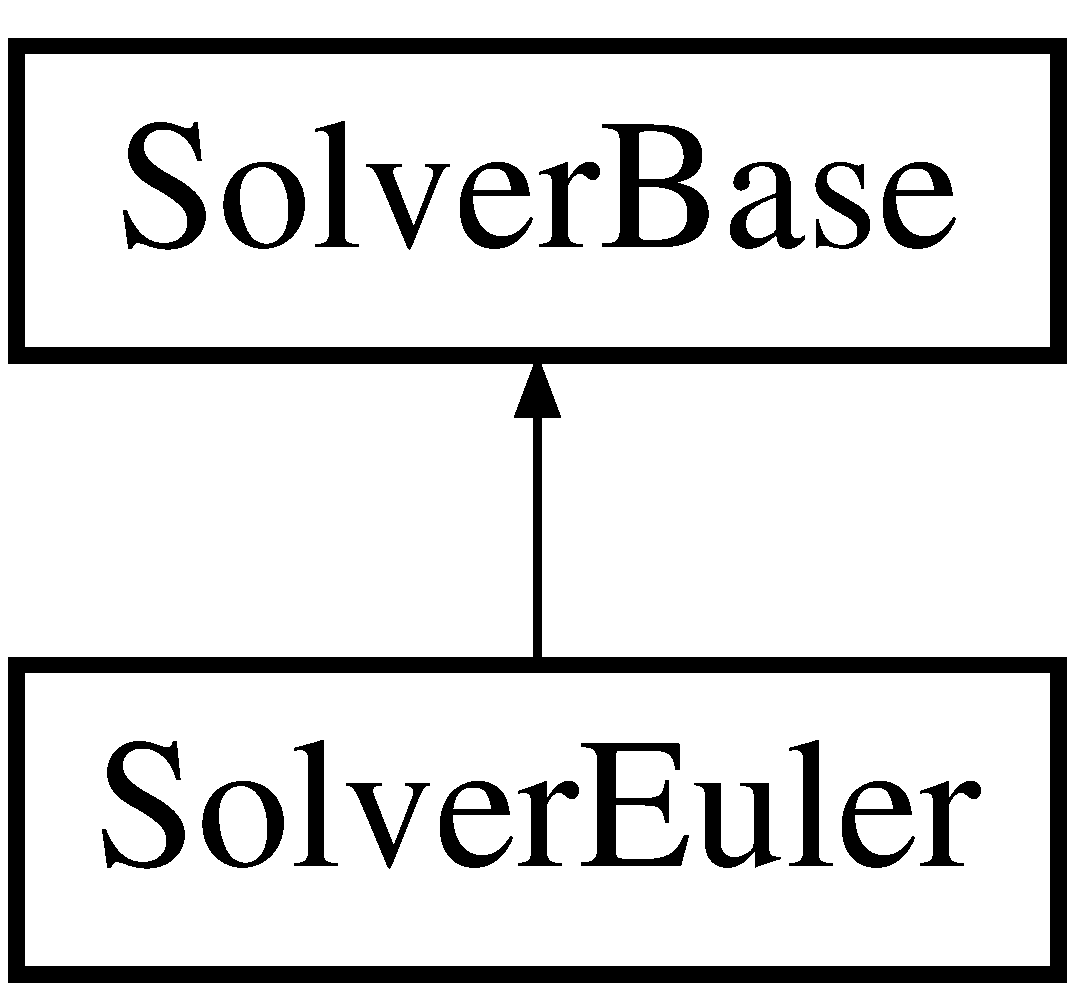
\includegraphics[height=2.000000cm]{class_solver_euler}
\end{center}
\end{figure}
\subsection*{Public Member Functions}
\begin{DoxyCompactItemize}
\item 
\mbox{\hyperlink{class_solver_euler_a775dd75545f3d9f69dab1c5ba2390edd}{Solver\+Euler}} (const \mbox{\hyperlink{class_f_e_mesh}{F\+E\+Mesh}} $\ast$mesh)
\begin{DoxyCompactList}\small\item\em Public Constructor. \end{DoxyCompactList}\item 
virtual \mbox{\hyperlink{class_solver_euler_a16777db2c518c46a6c41f5437376e479}{$\sim$\+Solver\+Euler}} ()
\begin{DoxyCompactList}\small\item\em Destructor. \end{DoxyCompactList}\item 
virtual void \mbox{\hyperlink{class_solver_euler_a64caa7276a35f9e5408bec75bc2d3189}{integrate\+In\+Time}} (double current\+Time, double dt)
\begin{DoxyCompactList}\small\item\em Time-\/step the solution. \end{DoxyCompactList}\item 
virtual void \mbox{\hyperlink{class_solver_euler_a5aa41447d61bd488d39ad12f97022473}{compute\+State}} (void)
\begin{DoxyCompactList}\small\item\em Compute the current state of the solution. \end{DoxyCompactList}\end{DoxyCompactItemize}


\subsection{Detailed Description}
Class for implementing compressible Euler equations on provided finite element mesh. See \mbox{\hyperlink{class_solver_base}{Solver\+Base}} for boundary conditions specifications. 

\subsection{Constructor \& Destructor Documentation}
\mbox{\Hypertarget{class_solver_euler_a775dd75545f3d9f69dab1c5ba2390edd}\label{class_solver_euler_a775dd75545f3d9f69dab1c5ba2390edd}} 
\index{Solver\+Euler@{Solver\+Euler}!Solver\+Euler@{Solver\+Euler}}
\index{Solver\+Euler@{Solver\+Euler}!Solver\+Euler@{Solver\+Euler}}
\subsubsection{\texorpdfstring{Solver\+Euler()}{SolverEuler()}}
{\footnotesize\ttfamily Solver\+Euler\+::\+Solver\+Euler (\begin{DoxyParamCaption}\item[{const \mbox{\hyperlink{class_f_e_mesh}{F\+E\+Mesh}} $\ast$}]{mesh }\end{DoxyParamCaption})}



Public Constructor. 


\begin{DoxyParams}{Parameters}
{\em mesh} & {\bfseries (const Mesh$\ast$)} \\
\hline
\end{DoxyParams}
\begin{DoxyReturn}{Returns}
Initialized \mbox{\hyperlink{class_solver_euler}{Solver\+Euler}} object 
\end{DoxyReturn}
\mbox{\Hypertarget{class_solver_euler_a16777db2c518c46a6c41f5437376e479}\label{class_solver_euler_a16777db2c518c46a6c41f5437376e479}} 
\index{Solver\+Euler@{Solver\+Euler}!````~Solver\+Euler@{$\sim$\+Solver\+Euler}}
\index{````~Solver\+Euler@{$\sim$\+Solver\+Euler}!Solver\+Euler@{Solver\+Euler}}
\subsubsection{\texorpdfstring{$\sim$\+Solver\+Euler()}{~SolverEuler()}}
{\footnotesize\ttfamily virtual Solver\+Euler\+::$\sim$\+Solver\+Euler (\begin{DoxyParamCaption}{ }\end{DoxyParamCaption})\hspace{0.3cm}{\ttfamily [inline]}, {\ttfamily [virtual]}}



Destructor. 

Note the destructor is virtual to ensure proper freeing of members if parent class delete is called 

\subsection{Member Function Documentation}
\mbox{\Hypertarget{class_solver_euler_a5aa41447d61bd488d39ad12f97022473}\label{class_solver_euler_a5aa41447d61bd488d39ad12f97022473}} 
\index{Solver\+Euler@{Solver\+Euler}!compute\+State@{compute\+State}}
\index{compute\+State@{compute\+State}!Solver\+Euler@{Solver\+Euler}}
\subsubsection{\texorpdfstring{compute\+State()}{computeState()}}
{\footnotesize\ttfamily virtual void Solver\+Euler\+::compute\+State (\begin{DoxyParamCaption}\item[{void}]{ }\end{DoxyParamCaption})\hspace{0.3cm}{\ttfamily [inline]}, {\ttfamily [virtual]}}



Compute the current state of the solution. 

This function computes the current state of the solution 
\begin{DoxyParams}{Parameters}
{\em None} & \\
\hline
\end{DoxyParams}
\begin{DoxyReturn}{Returns}
None 
\end{DoxyReturn}


Implements \mbox{\hyperlink{class_solver_base_a818006b80f29f641b6784905e1babe0f}{Solver\+Base}}.

\mbox{\Hypertarget{class_solver_euler_a64caa7276a35f9e5408bec75bc2d3189}\label{class_solver_euler_a64caa7276a35f9e5408bec75bc2d3189}} 
\index{Solver\+Euler@{Solver\+Euler}!integrate\+In\+Time@{integrate\+In\+Time}}
\index{integrate\+In\+Time@{integrate\+In\+Time}!Solver\+Euler@{Solver\+Euler}}
\subsubsection{\texorpdfstring{integrate\+In\+Time()}{integrateInTime()}}
{\footnotesize\ttfamily void Solver\+Euler\+::integrate\+In\+Time (\begin{DoxyParamCaption}\item[{double}]{current\+Time,  }\item[{double}]{dt }\end{DoxyParamCaption})\hspace{0.3cm}{\ttfamily [virtual]}}



Time-\/step the solution. 

\begin{DoxyRefDesc}{Todo}
\item[\mbox{\hyperlink{todo__todo000012}{Todo}}]This interface is deprecated, and should be implemented within base class\textquotesingle{} compute\+State function. \end{DoxyRefDesc}


The documentation for this class was generated from the following files\+:\begin{DoxyCompactItemize}
\item 
\mbox{\hyperlink{_solver_euler_8hpp}{Solver\+Euler.\+hpp}}\item 
\mbox{\hyperlink{_solver_euler_8cpp}{Solver\+Euler.\+cpp}}\end{DoxyCompactItemize}

\hypertarget{class_solver_poisson}{}\section{Solver\+Poisson Class Reference}
\label{class_solver_poisson}\index{Solver\+Poisson@{Solver\+Poisson}}
Inheritance diagram for Solver\+Poisson\+:\begin{figure}[H]
\begin{center}
\leavevmode
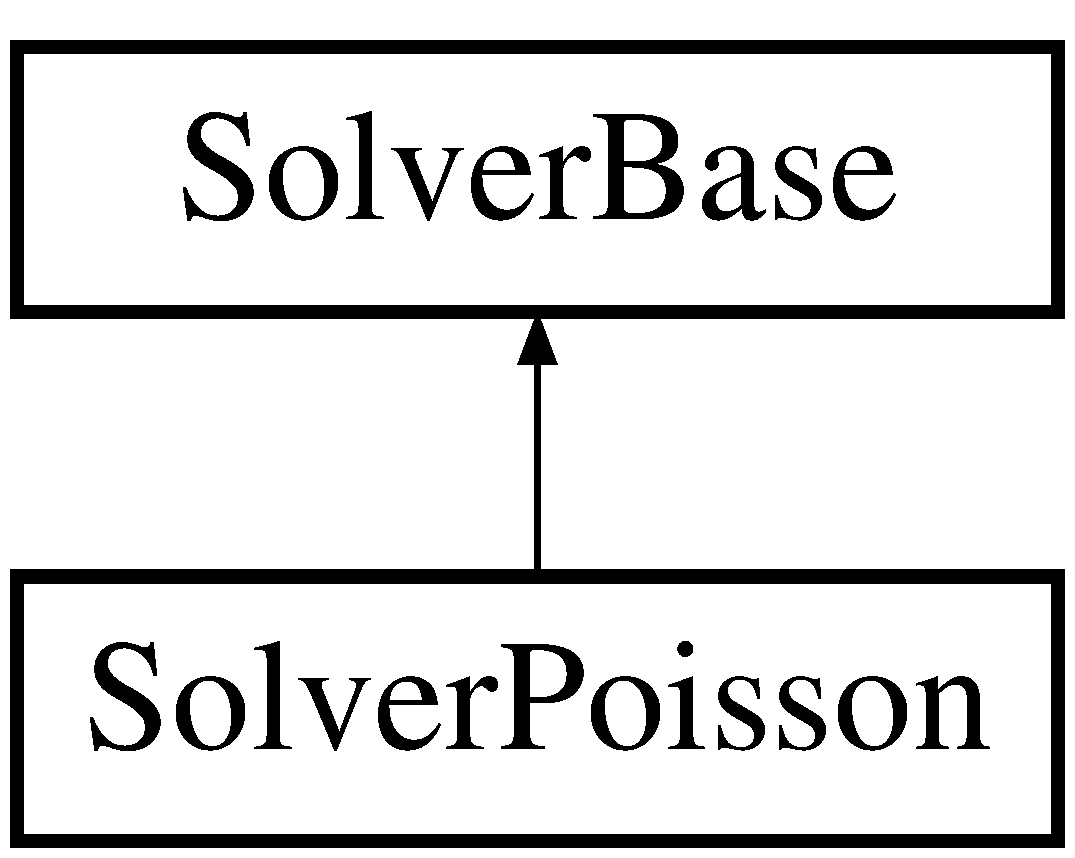
\includegraphics[height=2.000000cm]{class_solver_poisson}
\end{center}
\end{figure}
\subsection*{Additional Inherited Members}


The documentation for this class was generated from the following file\+:\begin{DoxyCompactItemize}
\item 
\mbox{\hyperlink{_solver_poisson_8hpp}{Solver\+Poisson.\+hpp}}\end{DoxyCompactItemize}

\chapter{File Documentation}
\hypertarget{cfgui_8py}{}\section{cfgui.\+py File Reference}
\label{cfgui_8py}\index{cfgui.\+py@{cfgui.\+py}}
\subsection*{Namespaces}
\begin{DoxyCompactItemize}
\item 
 \mbox{\hyperlink{namespacecfgui}{cfgui}}
\end{DoxyCompactItemize}
\subsection*{Variables}
\begin{DoxyCompactItemize}
\item 
\mbox{\hyperlink{namespacecfgui_ad0261b0d3cca8159d011afa3c17bd9f1}{cfgui.\+root}} = tk.\+Tk()
\item 
\mbox{\hyperlink{namespacecfgui_a64ae648845422a3c70e06f75eb5fa172}{cfgui.\+f}} = Figure(figsize=(6,5), dpi=150)
\item 
\mbox{\hyperlink{namespacecfgui_afa1e0012aec603eb6c61806994452873}{cfgui.\+a}} = f.\+add\+\_\+subplot(111)
\item 
string \mbox{\hyperlink{namespacecfgui_ae4078f684c5dfbf537a587c88b087e39}{cfgui.\+filename}} = \char`\"{}\char`\"{}
\item 
string \mbox{\hyperlink{namespacecfgui_adacec56309d4b55d655ac53531223503}{cfgui.\+newfilename}} = \char`\"{}\char`\"{}
\item 
int \mbox{\hyperlink{namespacecfgui_a4f032350a6dae97371e2e21bcc0223f3}{cfgui.\+filehandle}} = 0
\item 
list \mbox{\hyperlink{namespacecfgui_a4d1fd2c1f28a077f91899b4af9665928}{cfgui.\+active\+Node\+List}} = \mbox{[}$\,$\mbox{]}
\item 
int \mbox{\hyperlink{namespacecfgui_a69cb956a983205fbd404d059670db416}{cfgui.\+new\+Node\+ID}} = 0
\item 
int \mbox{\hyperlink{namespacecfgui_ade4f0d3b0706b49e072673e48b2ac242}{cfgui.\+unmeshed}} = 0
\item 
int \mbox{\hyperlink{namespacecfgui_aa3107f0b2f277f51f50bc28f5d93cb7e}{cfgui.\+editing}} = 0
\item 
\mbox{\hyperlink{namespacecfgui_aafee5f0725f5961d2bc6696ddac838ce}{cfgui.\+canvas}} = Figure\+Canvas\+Tk\+Agg(f, master=root)
\item 
\mbox{\hyperlink{namespacecfgui_ae9b6ae360c249a392d4154426dff9609}{cfgui.\+side}}
\item 
\mbox{\hyperlink{namespacecfgui_abdd84db69f76172a7b2e574cf726eb24}{cfgui.\+T\+OP}}
\item 
\mbox{\hyperlink{namespacecfgui_a86a27e16bd39f4f3228f753b3f04cb91}{cfgui.\+fill}}
\item 
\mbox{\hyperlink{namespacecfgui_ae68d5f9438e41baf4820d8044f868346}{cfgui.\+B\+O\+TH}}
\item 
\mbox{\hyperlink{namespacecfgui_a584b910dd9e596e04fe616d866f91ff2}{cfgui.\+expand}}
\item 
\mbox{\hyperlink{namespacecfgui_a7410773bac81022643bbb700b65ffd35}{cfgui.\+toolbar}} = Navigation\+Toolbar2\+Tk\+Agg(canvas,root)
\item 
\mbox{\hyperlink{namespacecfgui_a178f690140e4928e80ed598ebbbf6ec1}{cfgui.\+menu}} = Menu(root)
\item 
\mbox{\hyperlink{namespacecfgui_ae54e3f8d355a03929c89a227c506d39e}{cfgui.\+filemenu}} = Menu(menu)
\item 
\mbox{\hyperlink{namespacecfgui_a5bb1e89c42bd42a9baf53da59a27658d}{cfgui.\+label}}
\item 
\mbox{\hyperlink{namespacecfgui_a32a18002fc6635b3c814b5e9b329ec6b}{cfgui.\+command}}
\item 
\mbox{\hyperlink{namespacecfgui_aa44f9f5c68e640ec65a1a1c93e148982}{cfgui.\+accelerator}}
\item 
\mbox{\hyperlink{namespacecfgui_afef0987be82596ace82157e0682cac34}{cfgui.\+editmenu}} = Menu(menu)
\item 
\mbox{\hyperlink{namespacecfgui_a3a48ab8eff50c8134be0e6351bc9279d}{cfgui.\+helpmenu}} = Menu(menu)
\item 
\mbox{\hyperlink{namespacecfgui_a4cb6233c9db194dad78f3a686d22475c}{cfgui.\+mesh\+Button}} = tk.\+Button(master=root, text=\char`\"{}Mesh (\%s\%s)\char`\"{} \% (u\char`\"{}\textbackslash{}u2318\char`\"{},\char`\"{}M\char`\"{}), command=\+\_\+mesh)
\end{DoxyCompactItemize}

\hypertarget{_f_e_mesh_8cpp}{}\section{F\+E\+Mesh.\+cpp File Reference}
\label{_f_e_mesh_8cpp}\index{F\+E\+Mesh.\+cpp@{F\+E\+Mesh.\+cpp}}

\hypertarget{_f_e_mesh_8hpp}{}\section{F\+E\+Mesh.\+hpp File Reference}
\label{_f_e_mesh_8hpp}\index{F\+E\+Mesh.\+hpp@{F\+E\+Mesh.\+hpp}}
\subsection*{Classes}
\begin{DoxyCompactItemize}
\item 
class \mbox{\hyperlink{class_f_e_mesh}{F\+E\+Mesh}}
\end{DoxyCompactItemize}

\hypertarget{_includes_8hpp}{}\section{Includes.\+hpp File Reference}
\label{_includes_8hpp}\index{Includes.\+hpp@{Includes.\+hpp}}

\hypertarget{main_8cpp}{}\section{main.\+cpp File Reference}
\label{main_8cpp}\index{main.\+cpp@{main.\+cpp}}
\subsection*{Functions}
\begin{DoxyCompactItemize}
\item 
int \mbox{\hyperlink{main_8cpp_ac0f2228420376f4db7e1274f2b41667c}{main}} (int argc, const char $\ast$argv\mbox{[}$\,$\mbox{]})
\end{DoxyCompactItemize}


\subsection{Function Documentation}
\mbox{\Hypertarget{main_8cpp_ac0f2228420376f4db7e1274f2b41667c}\label{main_8cpp_ac0f2228420376f4db7e1274f2b41667c}} 
\index{main.\+cpp@{main.\+cpp}!main@{main}}
\index{main@{main}!main.\+cpp@{main.\+cpp}}
\subsubsection{\texorpdfstring{main()}{main()}}
{\footnotesize\ttfamily int main (\begin{DoxyParamCaption}\item[{int}]{argc,  }\item[{const char $\ast$}]{argv\mbox{[}$\,$\mbox{]} }\end{DoxyParamCaption})}


\hypertarget{_math_8cpp}{}\section{Math.\+cpp File Reference}
\label{_math_8cpp}\index{Math.\+cpp@{Math.\+cpp}}

\hypertarget{_math_8hpp}{}\section{Math.\+hpp File Reference}
\label{_math_8hpp}\index{Math.\+hpp@{Math.\+hpp}}
\subsection*{Classes}
\begin{DoxyCompactItemize}
\item 
class \mbox{\hyperlink{class_math_1_1_combinatorics}{Math\+::\+Combinatorics}}
\begin{DoxyCompactList}\small\item\em \mbox{\hyperlink{class_math_1_1_combinatorics}{Combinatorics}} class performs basic combinatorial operations. \end{DoxyCompactList}\item 
class \mbox{\hyperlink{class_math_1_1_function}{Math\+::\+Function}}
\begin{DoxyCompactList}\small\item\em This class associates a list of. \end{DoxyCompactList}\item 
class \mbox{\hyperlink{class_math_1_1_basis_el}{Math\+::\+Basis\+El}}
\begin{DoxyCompactList}\small\item\em Basis element class. \end{DoxyCompactList}\item 
class \mbox{\hyperlink{class_math_1_1_basis_rep}{Math\+::\+Basis\+Rep}}
\begin{DoxyCompactList}\small\item\em Basis element representation of a function. \end{DoxyCompactList}\end{DoxyCompactItemize}
\subsection*{Namespaces}
\begin{DoxyCompactItemize}
\item 
 \mbox{\hyperlink{namespace_math}{Math}}
\end{DoxyCompactItemize}

\hypertarget{_matrix_8cpp}{}\section{Matrix.\+cpp File Reference}
\label{_matrix_8cpp}\index{Matrix.\+cpp@{Matrix.\+cpp}}
\subsection*{Functions}
\begin{DoxyCompactItemize}
\item 
\mbox{\hyperlink{class_matrix}{Matrix}} \mbox{\hyperlink{_matrix_8cpp_ada4b4a55c64a37ec639de92e3bc61993}{eye}} (int n)
\item 
\mbox{\hyperlink{class_matrix}{Matrix}} \mbox{\hyperlink{_matrix_8cpp_a691ee4cd354731c3b0915799e04793fb}{ones}} (int num\+Rows, int num\+Cols=-\/1)
\item 
\mbox{\hyperlink{class_matrix}{Matrix}} \mbox{\hyperlink{_matrix_8cpp_a122abe6d89ed35706ff27abd384f96bc}{tri\+Diag}} (int n, double diag, double off\+Diag)
\item 
\mbox{\hyperlink{class_matrix}{Matrix}} \mbox{\hyperlink{_matrix_8cpp_a69677ca39fcad9f3d2ed1c013df19a2d}{comp\+Mat}} (std\+::vector$<$ double $>$ coefficients)
\item 
\mbox{\hyperlink{class_matrix}{Matrix}} \mbox{\hyperlink{_matrix_8cpp_aa2c60dc47762586cc2d67deac5aacb01}{rot\+Mat}} (double theta)
\item 
std\+::vector$<$ int $>$ \mbox{\hyperlink{_matrix_8cpp_af6d3c5d3d22c5f3f4a5fd47e3a7d3243}{index\+Vect}} (int n)
\item 
std\+::ostream \& \mbox{\hyperlink{_matrix_8cpp_ac7214274c9ef83ebef022af7225ac068}{operator$<$$<$}} (std\+::ostream \&os, const \mbox{\hyperlink{class_matrix}{Matrix}} A)
\item 
std\+::ostream \& \mbox{\hyperlink{_matrix_8cpp_a8bdcf56994dd828afb6662c681140623}{operator$<$$<$}} (std\+::ostream \&os, std\+::vector$<$ double $>$ vect)
\end{DoxyCompactItemize}


\subsection{Function Documentation}
\mbox{\Hypertarget{_matrix_8cpp_a69677ca39fcad9f3d2ed1c013df19a2d}\label{_matrix_8cpp_a69677ca39fcad9f3d2ed1c013df19a2d}} 
\index{Matrix.\+cpp@{Matrix.\+cpp}!comp\+Mat@{comp\+Mat}}
\index{comp\+Mat@{comp\+Mat}!Matrix.\+cpp@{Matrix.\+cpp}}
\subsubsection{\texorpdfstring{comp\+Mat()}{compMat()}}
{\footnotesize\ttfamily \mbox{\hyperlink{class_matrix}{Matrix}} comp\+Mat (\begin{DoxyParamCaption}\item[{std\+::vector$<$ double $>$}]{coefficients }\end{DoxyParamCaption})}

\mbox{\Hypertarget{_matrix_8cpp_ada4b4a55c64a37ec639de92e3bc61993}\label{_matrix_8cpp_ada4b4a55c64a37ec639de92e3bc61993}} 
\index{Matrix.\+cpp@{Matrix.\+cpp}!eye@{eye}}
\index{eye@{eye}!Matrix.\+cpp@{Matrix.\+cpp}}
\subsubsection{\texorpdfstring{eye()}{eye()}}
{\footnotesize\ttfamily \mbox{\hyperlink{class_matrix}{Matrix}} eye (\begin{DoxyParamCaption}\item[{int}]{n }\end{DoxyParamCaption})}

\mbox{\Hypertarget{_matrix_8cpp_af6d3c5d3d22c5f3f4a5fd47e3a7d3243}\label{_matrix_8cpp_af6d3c5d3d22c5f3f4a5fd47e3a7d3243}} 
\index{Matrix.\+cpp@{Matrix.\+cpp}!index\+Vect@{index\+Vect}}
\index{index\+Vect@{index\+Vect}!Matrix.\+cpp@{Matrix.\+cpp}}
\subsubsection{\texorpdfstring{index\+Vect()}{indexVect()}}
{\footnotesize\ttfamily std\+::vector$<$int$>$ index\+Vect (\begin{DoxyParamCaption}\item[{int}]{n }\end{DoxyParamCaption})}

\mbox{\Hypertarget{_matrix_8cpp_a691ee4cd354731c3b0915799e04793fb}\label{_matrix_8cpp_a691ee4cd354731c3b0915799e04793fb}} 
\index{Matrix.\+cpp@{Matrix.\+cpp}!ones@{ones}}
\index{ones@{ones}!Matrix.\+cpp@{Matrix.\+cpp}}
\subsubsection{\texorpdfstring{ones()}{ones()}}
{\footnotesize\ttfamily \mbox{\hyperlink{class_matrix}{Matrix}} ones (\begin{DoxyParamCaption}\item[{int}]{num\+Rows,  }\item[{int}]{num\+Cols = {\ttfamily -\/1} }\end{DoxyParamCaption})}

\mbox{\Hypertarget{_matrix_8cpp_ac7214274c9ef83ebef022af7225ac068}\label{_matrix_8cpp_ac7214274c9ef83ebef022af7225ac068}} 
\index{Matrix.\+cpp@{Matrix.\+cpp}!operator$<$$<$@{operator$<$$<$}}
\index{operator$<$$<$@{operator$<$$<$}!Matrix.\+cpp@{Matrix.\+cpp}}
\subsubsection{\texorpdfstring{operator$<$$<$()}{operator<<()}\hspace{0.1cm}{\footnotesize\ttfamily [1/2]}}
{\footnotesize\ttfamily std\+::ostream\& operator$<$$<$ (\begin{DoxyParamCaption}\item[{std\+::ostream \&}]{os,  }\item[{const \mbox{\hyperlink{class_matrix}{Matrix}}}]{A }\end{DoxyParamCaption})}

\mbox{\Hypertarget{_matrix_8cpp_a8bdcf56994dd828afb6662c681140623}\label{_matrix_8cpp_a8bdcf56994dd828afb6662c681140623}} 
\index{Matrix.\+cpp@{Matrix.\+cpp}!operator$<$$<$@{operator$<$$<$}}
\index{operator$<$$<$@{operator$<$$<$}!Matrix.\+cpp@{Matrix.\+cpp}}
\subsubsection{\texorpdfstring{operator$<$$<$()}{operator<<()}\hspace{0.1cm}{\footnotesize\ttfamily [2/2]}}
{\footnotesize\ttfamily std\+::ostream\& operator$<$$<$ (\begin{DoxyParamCaption}\item[{std\+::ostream \&}]{os,  }\item[{std\+::vector$<$ double $>$}]{vect }\end{DoxyParamCaption})}

\mbox{\Hypertarget{_matrix_8cpp_aa2c60dc47762586cc2d67deac5aacb01}\label{_matrix_8cpp_aa2c60dc47762586cc2d67deac5aacb01}} 
\index{Matrix.\+cpp@{Matrix.\+cpp}!rot\+Mat@{rot\+Mat}}
\index{rot\+Mat@{rot\+Mat}!Matrix.\+cpp@{Matrix.\+cpp}}
\subsubsection{\texorpdfstring{rot\+Mat()}{rotMat()}}
{\footnotesize\ttfamily \mbox{\hyperlink{class_matrix}{Matrix}} rot\+Mat (\begin{DoxyParamCaption}\item[{double}]{theta }\end{DoxyParamCaption})}

\mbox{\Hypertarget{_matrix_8cpp_a122abe6d89ed35706ff27abd384f96bc}\label{_matrix_8cpp_a122abe6d89ed35706ff27abd384f96bc}} 
\index{Matrix.\+cpp@{Matrix.\+cpp}!tri\+Diag@{tri\+Diag}}
\index{tri\+Diag@{tri\+Diag}!Matrix.\+cpp@{Matrix.\+cpp}}
\subsubsection{\texorpdfstring{tri\+Diag()}{triDiag()}}
{\footnotesize\ttfamily \mbox{\hyperlink{class_matrix}{Matrix}} tri\+Diag (\begin{DoxyParamCaption}\item[{int}]{n,  }\item[{double}]{diag,  }\item[{double}]{off\+Diag }\end{DoxyParamCaption})}


\hypertarget{_matrix_8hpp}{}\section{Matrix.\+hpp File Reference}
\label{_matrix_8hpp}\index{Matrix.\+hpp@{Matrix.\+hpp}}
\subsection*{Classes}
\begin{DoxyCompactItemize}
\item 
class \mbox{\hyperlink{class_matrix}{Matrix}}
\end{DoxyCompactItemize}

\hypertarget{_mesh_8cpp}{}\section{Mesh.\+cpp File Reference}
\label{_mesh_8cpp}\index{Mesh.\+cpp@{Mesh.\+cpp}}

\hypertarget{_mesh_8hpp}{}\section{Mesh.\+hpp File Reference}
\label{_mesh_8hpp}\index{Mesh.\+hpp@{Mesh.\+hpp}}
\subsection*{Classes}
\begin{DoxyCompactItemize}
\item 
class \mbox{\hyperlink{class_mesh}{Mesh}}
\begin{DoxyCompactList}\small\item\em \mbox{\hyperlink{class_mesh}{Mesh}} class generates and stores a 2D mesh from an input grid points file. \end{DoxyCompactList}\item 
class \mbox{\hyperlink{class_node}{Node}}
\begin{DoxyCompactList}\small\item\em \mbox{\hyperlink{class_node}{Node}} class provides A\+PI for a vertex object in a \mbox{\hyperlink{class_mesh}{Mesh}}. \end{DoxyCompactList}\item 
class \mbox{\hyperlink{class_facet}{Facet}}
\begin{DoxyCompactList}\small\item\em \mbox{\hyperlink{class_facet}{Facet}} object is a triangle defined by three \mbox{\hyperlink{class_node}{Node}} objects. \end{DoxyCompactList}\end{DoxyCompactItemize}
\subsection*{Functions}
\begin{DoxyCompactItemize}
\item 
void \mbox{\hyperlink{_mesh_8hpp_a47943ea5ef9ca7fe072bed4c62c757ce}{sort\+Nodes\+By\+Angle}} (std\+::vector$<$ \mbox{\hyperlink{class_node}{Node}} $\ast$$>$ \&node\+List)
\item 
bool \mbox{\hyperlink{_mesh_8hpp_a70c68e42378612e2400bbeda26d60a8e}{compare\+Nodes}} (\mbox{\hyperlink{class_node}{Node}} $\ast$const a, \mbox{\hyperlink{class_node}{Node}} $\ast$const b)
\end{DoxyCompactItemize}


\subsection{Function Documentation}
\mbox{\Hypertarget{_mesh_8hpp_a70c68e42378612e2400bbeda26d60a8e}\label{_mesh_8hpp_a70c68e42378612e2400bbeda26d60a8e}} 
\index{Mesh.\+hpp@{Mesh.\+hpp}!compare\+Nodes@{compare\+Nodes}}
\index{compare\+Nodes@{compare\+Nodes}!Mesh.\+hpp@{Mesh.\+hpp}}
\subsubsection{\texorpdfstring{compare\+Nodes()}{compareNodes()}}
{\footnotesize\ttfamily bool compare\+Nodes (\begin{DoxyParamCaption}\item[{\mbox{\hyperlink{class_node}{Node}} $\ast$const}]{a,  }\item[{\mbox{\hyperlink{class_node}{Node}} $\ast$const}]{b }\end{DoxyParamCaption})}

\mbox{\Hypertarget{_mesh_8hpp_a47943ea5ef9ca7fe072bed4c62c757ce}\label{_mesh_8hpp_a47943ea5ef9ca7fe072bed4c62c757ce}} 
\index{Mesh.\+hpp@{Mesh.\+hpp}!sort\+Nodes\+By\+Angle@{sort\+Nodes\+By\+Angle}}
\index{sort\+Nodes\+By\+Angle@{sort\+Nodes\+By\+Angle}!Mesh.\+hpp@{Mesh.\+hpp}}
\subsubsection{\texorpdfstring{sort\+Nodes\+By\+Angle()}{sortNodesByAngle()}}
{\footnotesize\ttfamily void sort\+Nodes\+By\+Angle (\begin{DoxyParamCaption}\item[{std\+::vector$<$ \mbox{\hyperlink{class_node}{Node}} $\ast$$>$ \&}]{node\+List }\end{DoxyParamCaption})}


\hypertarget{_options_8cpp}{}\section{Options.\+cpp File Reference}
\label{_options_8cpp}\index{Options.\+cpp@{Options.\+cpp}}

\hypertarget{_options_8hpp}{}\section{Options.\+hpp File Reference}
\label{_options_8hpp}\index{Options.\+hpp@{Options.\+hpp}}
\subsection*{Classes}
\begin{DoxyCompactItemize}
\item 
class \mbox{\hyperlink{class_options}{Options}}
\end{DoxyCompactItemize}

\hypertarget{_solver_8cpp}{}\section{Solver.\+cpp File Reference}
\label{_solver_8cpp}\index{Solver.\+cpp@{Solver.\+cpp}}

\hypertarget{_solver_8hpp}{}\section{Solver.\+hpp File Reference}
\label{_solver_8hpp}\index{Solver.\+hpp@{Solver.\+hpp}}
\subsection*{Classes}
\begin{DoxyCompactItemize}
\item 
class \mbox{\hyperlink{class_solver_base}{Solver\+Base}}
\end{DoxyCompactItemize}

\hypertarget{_solver_euler_8cpp}{}\section{Solver\+Euler.\+cpp File Reference}
\label{_solver_euler_8cpp}\index{Solver\+Euler.\+cpp@{Solver\+Euler.\+cpp}}

\hypertarget{_solver_euler_8hpp}{}\section{Solver\+Euler.\+hpp File Reference}
\label{_solver_euler_8hpp}\index{Solver\+Euler.\+hpp@{Solver\+Euler.\+hpp}}
\subsection*{Classes}
\begin{DoxyCompactItemize}
\item 
class \mbox{\hyperlink{class_solver_euler}{Solver\+Euler}}
\end{DoxyCompactItemize}

\hypertarget{_solver_poisson_8cpp}{}\section{Solver\+Poisson.\+cpp File Reference}
\label{_solver_poisson_8cpp}\index{Solver\+Poisson.\+cpp@{Solver\+Poisson.\+cpp}}

\hypertarget{_solver_poisson_8hpp}{}\section{Solver\+Poisson.\+hpp File Reference}
\label{_solver_poisson_8hpp}\index{Solver\+Poisson.\+hpp@{Solver\+Poisson.\+hpp}}
\subsection*{Classes}
\begin{DoxyCompactItemize}
\item 
class \mbox{\hyperlink{class_solver_poisson}{Solver\+Poisson}}
\end{DoxyCompactItemize}

\hypertarget{_vect_ops_8cpp}{}\section{Vect\+Ops.\+cpp File Reference}
\label{_vect_ops_8cpp}\index{Vect\+Ops.\+cpp@{Vect\+Ops.\+cpp}}
\subsection*{Functions}
\begin{DoxyCompactItemize}
\item 
std\+::vector$<$ double $>$ \mbox{\hyperlink{_vect_ops_8cpp_ae81724e95cc778eba1c19eef67db16ca}{operator+}} (std\+::vector$<$ double $>$ lhs, std\+::vector$<$ double $>$ rhs)
\item 
std\+::vector$<$ double $>$ \mbox{\hyperlink{_vect_ops_8cpp_a28d00bc4ffde1f4718027efd3d2062fa}{operator-\/}} (std\+::vector$<$ double $>$ lhs, std\+::vector$<$ double $>$ rhs)
\item 
double \mbox{\hyperlink{_vect_ops_8cpp_a3a5143035ddf186131893c5e07485860}{dot}} (std\+::vector$<$ double $>$ u, std\+::vector$<$ double $>$ v)
\item 
double \mbox{\hyperlink{_vect_ops_8cpp_a5e3a2af5c7902cdfb1228f10647032e2}{norm}} (std\+::vector$<$ double $>$ u, double p)
\item 
std\+::vector$<$ double $>$ \mbox{\hyperlink{_vect_ops_8cpp_a13a02049d4b44c2605f77caf368b94a0}{scale}} (std\+::vector$<$ double $>$ u, double c)
\item 
std\+::vector$<$ double $>$ \mbox{\hyperlink{_vect_ops_8cpp_a189d9161377fa8de27f48140da0378c0}{vect\+Pow}} (std\+::vector$<$ double $>$ u, double p)
\item 
{\footnotesize template$<$class T $>$ }\\std\+::vector$<$ T $\ast$ $>$ \mbox{\hyperlink{_vect_ops_8cpp_aad801f3d8698e1bb15e7b5a8a94ed7af}{range}} (std\+::vector$<$ T $\ast$$>$ u, size\+\_\+t min, size\+\_\+t max)
\item 
{\footnotesize template$<$class T $>$ }\\std\+::vector$<$ T $\ast$ $>$ \mbox{\hyperlink{_vect_ops_8cpp_aece55178fa72cf8cd94677b977b2cf01}{subind}} (std\+::vector$<$ T $\ast$$>$ u, std\+::vector$<$ int $>$ inds)
\item 
{\footnotesize template$<$class T $>$ }\\std\+::vector$<$ T $\ast$ $>$ \mbox{\hyperlink{_vect_ops_8cpp_a5b91beaeed874fe6912782b5db372dcb}{cat}} (std\+::vector$<$ T $\ast$$>$ u, std\+::vector$<$ T $\ast$$>$ v)
\item 
{\footnotesize template$<$class T $>$ }\\std\+::vector$<$ T $\ast$ $>$ \mbox{\hyperlink{_vect_ops_8cpp_a0194dbced2a549ceb0f4a4efe1afc08d}{rm\+El}} (std\+::vector$<$ T $\ast$$>$ u, size\+\_\+t ind2rm)
\item 
{\footnotesize template$<$class T $>$ }\\void \mbox{\hyperlink{_vect_ops_8cpp_a6a269e1da45ae7e47221131a52b3fe88}{rev\+Sort}} (std\+::vector$<$ T $\ast$$>$ u)
\item 
template std\+::vector$<$ \mbox{\hyperlink{class_node}{Node}} $\ast$ $>$ \mbox{\hyperlink{_vect_ops_8cpp_abfb48e7a363f600ab75965d902c5638a}{range}} (std\+::vector$<$ \mbox{\hyperlink{class_node}{Node}} $\ast$$>$, size\+\_\+t, size\+\_\+t)
\item 
template std\+::vector$<$ \mbox{\hyperlink{class_node}{Node}} $\ast$ $>$ \mbox{\hyperlink{_vect_ops_8cpp_a2c7cf4eeb17ae6b95361226420bbf5d8}{cat}} (std\+::vector$<$ \mbox{\hyperlink{class_node}{Node}} $\ast$$>$, std\+::vector$<$ \mbox{\hyperlink{class_node}{Node}} $\ast$$>$)
\item 
template std\+::vector$<$ \mbox{\hyperlink{class_facet}{Facet}} $\ast$ $>$ \mbox{\hyperlink{_vect_ops_8cpp_aca9814cfa5f4e1e0eb5c6be77dc3d2f2}{cat}} (std\+::vector$<$ \mbox{\hyperlink{class_facet}{Facet}} $\ast$$>$, std\+::vector$<$ \mbox{\hyperlink{class_facet}{Facet}} $\ast$$>$)
\item 
template std\+::vector$<$ \mbox{\hyperlink{class_node}{Node}} $\ast$ $>$ \mbox{\hyperlink{_vect_ops_8cpp_a29e4f478fd231dfb88a98becc559e98c}{rm\+El}} (std\+::vector$<$ \mbox{\hyperlink{class_node}{Node}} $\ast$$>$, size\+\_\+t)
\item 
template void \mbox{\hyperlink{_vect_ops_8cpp_a8b8f13b2cb412e6d09ee216c08285816}{rev\+Sort}} (std\+::vector$<$ \mbox{\hyperlink{class_node}{Node}} $\ast$$>$)
\end{DoxyCompactItemize}


\subsection{Function Documentation}
\mbox{\Hypertarget{_vect_ops_8cpp_a5b91beaeed874fe6912782b5db372dcb}\label{_vect_ops_8cpp_a5b91beaeed874fe6912782b5db372dcb}} 
\index{Vect\+Ops.\+cpp@{Vect\+Ops.\+cpp}!cat@{cat}}
\index{cat@{cat}!Vect\+Ops.\+cpp@{Vect\+Ops.\+cpp}}
\subsubsection{\texorpdfstring{cat()}{cat()}\hspace{0.1cm}{\footnotesize\ttfamily [1/3]}}
{\footnotesize\ttfamily template$<$class T $>$ \\
std\+::vector$<$T$\ast$$>$ cat (\begin{DoxyParamCaption}\item[{std\+::vector$<$ T $\ast$$>$}]{u,  }\item[{std\+::vector$<$ T $\ast$$>$}]{v }\end{DoxyParamCaption})}

\mbox{\Hypertarget{_vect_ops_8cpp_a2c7cf4eeb17ae6b95361226420bbf5d8}\label{_vect_ops_8cpp_a2c7cf4eeb17ae6b95361226420bbf5d8}} 
\index{Vect\+Ops.\+cpp@{Vect\+Ops.\+cpp}!cat@{cat}}
\index{cat@{cat}!Vect\+Ops.\+cpp@{Vect\+Ops.\+cpp}}
\subsubsection{\texorpdfstring{cat()}{cat()}\hspace{0.1cm}{\footnotesize\ttfamily [2/3]}}
{\footnotesize\ttfamily template std\+::vector$<$\mbox{\hyperlink{class_node}{Node}}$\ast$$>$ cat (\begin{DoxyParamCaption}\item[{std\+::vector$<$ \mbox{\hyperlink{class_node}{Node}} $\ast$$>$}]{,  }\item[{std\+::vector$<$ \mbox{\hyperlink{class_node}{Node}} $\ast$$>$}]{ }\end{DoxyParamCaption})}

\mbox{\Hypertarget{_vect_ops_8cpp_aca9814cfa5f4e1e0eb5c6be77dc3d2f2}\label{_vect_ops_8cpp_aca9814cfa5f4e1e0eb5c6be77dc3d2f2}} 
\index{Vect\+Ops.\+cpp@{Vect\+Ops.\+cpp}!cat@{cat}}
\index{cat@{cat}!Vect\+Ops.\+cpp@{Vect\+Ops.\+cpp}}
\subsubsection{\texorpdfstring{cat()}{cat()}\hspace{0.1cm}{\footnotesize\ttfamily [3/3]}}
{\footnotesize\ttfamily template std\+::vector$<$\mbox{\hyperlink{class_facet}{Facet}}$\ast$$>$ cat (\begin{DoxyParamCaption}\item[{std\+::vector$<$ \mbox{\hyperlink{class_facet}{Facet}} $\ast$$>$}]{,  }\item[{std\+::vector$<$ \mbox{\hyperlink{class_facet}{Facet}} $\ast$$>$}]{ }\end{DoxyParamCaption})}

\mbox{\Hypertarget{_vect_ops_8cpp_a3a5143035ddf186131893c5e07485860}\label{_vect_ops_8cpp_a3a5143035ddf186131893c5e07485860}} 
\index{Vect\+Ops.\+cpp@{Vect\+Ops.\+cpp}!dot@{dot}}
\index{dot@{dot}!Vect\+Ops.\+cpp@{Vect\+Ops.\+cpp}}
\subsubsection{\texorpdfstring{dot()}{dot()}}
{\footnotesize\ttfamily double dot (\begin{DoxyParamCaption}\item[{std\+::vector$<$ double $>$}]{u,  }\item[{std\+::vector$<$ double $>$}]{v }\end{DoxyParamCaption})}

\mbox{\Hypertarget{_vect_ops_8cpp_a5e3a2af5c7902cdfb1228f10647032e2}\label{_vect_ops_8cpp_a5e3a2af5c7902cdfb1228f10647032e2}} 
\index{Vect\+Ops.\+cpp@{Vect\+Ops.\+cpp}!norm@{norm}}
\index{norm@{norm}!Vect\+Ops.\+cpp@{Vect\+Ops.\+cpp}}
\subsubsection{\texorpdfstring{norm()}{norm()}}
{\footnotesize\ttfamily double norm (\begin{DoxyParamCaption}\item[{std\+::vector$<$ double $>$}]{u,  }\item[{double}]{p }\end{DoxyParamCaption})}

\mbox{\Hypertarget{_vect_ops_8cpp_ae81724e95cc778eba1c19eef67db16ca}\label{_vect_ops_8cpp_ae81724e95cc778eba1c19eef67db16ca}} 
\index{Vect\+Ops.\+cpp@{Vect\+Ops.\+cpp}!operator+@{operator+}}
\index{operator+@{operator+}!Vect\+Ops.\+cpp@{Vect\+Ops.\+cpp}}
\subsubsection{\texorpdfstring{operator+()}{operator+()}}
{\footnotesize\ttfamily std\+::vector$<$double$>$ operator+ (\begin{DoxyParamCaption}\item[{std\+::vector$<$ double $>$}]{lhs,  }\item[{std\+::vector$<$ double $>$}]{rhs }\end{DoxyParamCaption})}

\mbox{\Hypertarget{_vect_ops_8cpp_a28d00bc4ffde1f4718027efd3d2062fa}\label{_vect_ops_8cpp_a28d00bc4ffde1f4718027efd3d2062fa}} 
\index{Vect\+Ops.\+cpp@{Vect\+Ops.\+cpp}!operator-\/@{operator-\/}}
\index{operator-\/@{operator-\/}!Vect\+Ops.\+cpp@{Vect\+Ops.\+cpp}}
\subsubsection{\texorpdfstring{operator-\/()}{operator-()}}
{\footnotesize\ttfamily std\+::vector$<$double$>$ operator-\/ (\begin{DoxyParamCaption}\item[{std\+::vector$<$ double $>$}]{lhs,  }\item[{std\+::vector$<$ double $>$}]{rhs }\end{DoxyParamCaption})}

\mbox{\Hypertarget{_vect_ops_8cpp_aad801f3d8698e1bb15e7b5a8a94ed7af}\label{_vect_ops_8cpp_aad801f3d8698e1bb15e7b5a8a94ed7af}} 
\index{Vect\+Ops.\+cpp@{Vect\+Ops.\+cpp}!range@{range}}
\index{range@{range}!Vect\+Ops.\+cpp@{Vect\+Ops.\+cpp}}
\subsubsection{\texorpdfstring{range()}{range()}\hspace{0.1cm}{\footnotesize\ttfamily [1/2]}}
{\footnotesize\ttfamily template$<$class T $>$ \\
std\+::vector$<$T$\ast$$>$ range (\begin{DoxyParamCaption}\item[{std\+::vector$<$ T $\ast$$>$}]{u,  }\item[{size\+\_\+t}]{min,  }\item[{size\+\_\+t}]{max }\end{DoxyParamCaption})}

\mbox{\Hypertarget{_vect_ops_8cpp_abfb48e7a363f600ab75965d902c5638a}\label{_vect_ops_8cpp_abfb48e7a363f600ab75965d902c5638a}} 
\index{Vect\+Ops.\+cpp@{Vect\+Ops.\+cpp}!range@{range}}
\index{range@{range}!Vect\+Ops.\+cpp@{Vect\+Ops.\+cpp}}
\subsubsection{\texorpdfstring{range()}{range()}\hspace{0.1cm}{\footnotesize\ttfamily [2/2]}}
{\footnotesize\ttfamily template std\+::vector$<$\mbox{\hyperlink{class_node}{Node}}$\ast$$>$ range (\begin{DoxyParamCaption}\item[{std\+::vector$<$ \mbox{\hyperlink{class_node}{Node}} $\ast$$>$}]{,  }\item[{size\+\_\+t}]{,  }\item[{size\+\_\+t}]{ }\end{DoxyParamCaption})}

\mbox{\Hypertarget{_vect_ops_8cpp_a6a269e1da45ae7e47221131a52b3fe88}\label{_vect_ops_8cpp_a6a269e1da45ae7e47221131a52b3fe88}} 
\index{Vect\+Ops.\+cpp@{Vect\+Ops.\+cpp}!rev\+Sort@{rev\+Sort}}
\index{rev\+Sort@{rev\+Sort}!Vect\+Ops.\+cpp@{Vect\+Ops.\+cpp}}
\subsubsection{\texorpdfstring{rev\+Sort()}{revSort()}\hspace{0.1cm}{\footnotesize\ttfamily [1/2]}}
{\footnotesize\ttfamily template$<$class T $>$ \\
void rev\+Sort (\begin{DoxyParamCaption}\item[{std\+::vector$<$ T $\ast$$>$}]{u }\end{DoxyParamCaption})}

\mbox{\Hypertarget{_vect_ops_8cpp_a8b8f13b2cb412e6d09ee216c08285816}\label{_vect_ops_8cpp_a8b8f13b2cb412e6d09ee216c08285816}} 
\index{Vect\+Ops.\+cpp@{Vect\+Ops.\+cpp}!rev\+Sort@{rev\+Sort}}
\index{rev\+Sort@{rev\+Sort}!Vect\+Ops.\+cpp@{Vect\+Ops.\+cpp}}
\subsubsection{\texorpdfstring{rev\+Sort()}{revSort()}\hspace{0.1cm}{\footnotesize\ttfamily [2/2]}}
{\footnotesize\ttfamily template void rev\+Sort (\begin{DoxyParamCaption}\item[{std\+::vector$<$ \mbox{\hyperlink{class_node}{Node}} $\ast$$>$}]{ }\end{DoxyParamCaption})}

\mbox{\Hypertarget{_vect_ops_8cpp_a0194dbced2a549ceb0f4a4efe1afc08d}\label{_vect_ops_8cpp_a0194dbced2a549ceb0f4a4efe1afc08d}} 
\index{Vect\+Ops.\+cpp@{Vect\+Ops.\+cpp}!rm\+El@{rm\+El}}
\index{rm\+El@{rm\+El}!Vect\+Ops.\+cpp@{Vect\+Ops.\+cpp}}
\subsubsection{\texorpdfstring{rm\+El()}{rmEl()}\hspace{0.1cm}{\footnotesize\ttfamily [1/2]}}
{\footnotesize\ttfamily template$<$class T $>$ \\
std\+::vector$<$T$\ast$$>$ rm\+El (\begin{DoxyParamCaption}\item[{std\+::vector$<$ T $\ast$$>$}]{u,  }\item[{size\+\_\+t}]{ind2rm }\end{DoxyParamCaption})}

\mbox{\Hypertarget{_vect_ops_8cpp_a29e4f478fd231dfb88a98becc559e98c}\label{_vect_ops_8cpp_a29e4f478fd231dfb88a98becc559e98c}} 
\index{Vect\+Ops.\+cpp@{Vect\+Ops.\+cpp}!rm\+El@{rm\+El}}
\index{rm\+El@{rm\+El}!Vect\+Ops.\+cpp@{Vect\+Ops.\+cpp}}
\subsubsection{\texorpdfstring{rm\+El()}{rmEl()}\hspace{0.1cm}{\footnotesize\ttfamily [2/2]}}
{\footnotesize\ttfamily template std\+::vector$<$\mbox{\hyperlink{class_node}{Node}}$\ast$$>$ rm\+El (\begin{DoxyParamCaption}\item[{std\+::vector$<$ \mbox{\hyperlink{class_node}{Node}} $\ast$$>$}]{,  }\item[{size\+\_\+t}]{ }\end{DoxyParamCaption})}

\mbox{\Hypertarget{_vect_ops_8cpp_a13a02049d4b44c2605f77caf368b94a0}\label{_vect_ops_8cpp_a13a02049d4b44c2605f77caf368b94a0}} 
\index{Vect\+Ops.\+cpp@{Vect\+Ops.\+cpp}!scale@{scale}}
\index{scale@{scale}!Vect\+Ops.\+cpp@{Vect\+Ops.\+cpp}}
\subsubsection{\texorpdfstring{scale()}{scale()}}
{\footnotesize\ttfamily std\+::vector$<$double$>$ scale (\begin{DoxyParamCaption}\item[{std\+::vector$<$ double $>$}]{u,  }\item[{double}]{c }\end{DoxyParamCaption})}

\mbox{\Hypertarget{_vect_ops_8cpp_aece55178fa72cf8cd94677b977b2cf01}\label{_vect_ops_8cpp_aece55178fa72cf8cd94677b977b2cf01}} 
\index{Vect\+Ops.\+cpp@{Vect\+Ops.\+cpp}!subind@{subind}}
\index{subind@{subind}!Vect\+Ops.\+cpp@{Vect\+Ops.\+cpp}}
\subsubsection{\texorpdfstring{subind()}{subind()}}
{\footnotesize\ttfamily template$<$class T $>$ \\
std\+::vector$<$T$\ast$$>$ subind (\begin{DoxyParamCaption}\item[{std\+::vector$<$ T $\ast$$>$}]{u,  }\item[{std\+::vector$<$ int $>$}]{inds }\end{DoxyParamCaption})}

\mbox{\Hypertarget{_vect_ops_8cpp_a189d9161377fa8de27f48140da0378c0}\label{_vect_ops_8cpp_a189d9161377fa8de27f48140da0378c0}} 
\index{Vect\+Ops.\+cpp@{Vect\+Ops.\+cpp}!vect\+Pow@{vect\+Pow}}
\index{vect\+Pow@{vect\+Pow}!Vect\+Ops.\+cpp@{Vect\+Ops.\+cpp}}
\subsubsection{\texorpdfstring{vect\+Pow()}{vectPow()}}
{\footnotesize\ttfamily std\+::vector$<$double$>$ vect\+Pow (\begin{DoxyParamCaption}\item[{std\+::vector$<$ double $>$}]{u,  }\item[{double}]{p }\end{DoxyParamCaption})}


\hypertarget{_vect_ops_8hpp}{}\section{Vect\+Ops.\+hpp File Reference}
\label{_vect_ops_8hpp}\index{Vect\+Ops.\+hpp@{Vect\+Ops.\+hpp}}
\subsection*{Functions}
\begin{DoxyCompactItemize}
\item 
std\+::vector$<$ double $>$ \mbox{\hyperlink{_vect_ops_8hpp_ae81724e95cc778eba1c19eef67db16ca}{operator+}} (std\+::vector$<$ double $>$ lhs, std\+::vector$<$ double $>$ rhs)
\item 
std\+::vector$<$ double $>$ \mbox{\hyperlink{_vect_ops_8hpp_a28d00bc4ffde1f4718027efd3d2062fa}{operator-\/}} (std\+::vector$<$ double $>$ lhs, std\+::vector$<$ double $>$ rhs)
\item 
double \mbox{\hyperlink{_vect_ops_8hpp_a3a5143035ddf186131893c5e07485860}{dot}} (std\+::vector$<$ double $>$ u, std\+::vector$<$ double $>$ v)
\item 
double \mbox{\hyperlink{_vect_ops_8hpp_a7fa9e5a0b18885f8c572a00579800b37}{norm}} (std\+::vector$<$ double $>$ u, double p=2)
\item 
std\+::vector$<$ double $>$ \mbox{\hyperlink{_vect_ops_8hpp_a13a02049d4b44c2605f77caf368b94a0}{scale}} (std\+::vector$<$ double $>$ u, double c)
\item 
std\+::vector$<$ double $>$ \mbox{\hyperlink{_vect_ops_8hpp_a189d9161377fa8de27f48140da0378c0}{vect\+Pow}} (std\+::vector$<$ double $>$ u, double p)
\item 
{\footnotesize template$<$class T $>$ }\\std\+::vector$<$ T $\ast$ $>$ \mbox{\hyperlink{_vect_ops_8hpp_aad801f3d8698e1bb15e7b5a8a94ed7af}{range}} (std\+::vector$<$ T $\ast$$>$ u, size\+\_\+t min, size\+\_\+t max)
\item 
{\footnotesize template$<$class T $>$ }\\std\+::vector$<$ T $\ast$ $>$ \mbox{\hyperlink{_vect_ops_8hpp_aece55178fa72cf8cd94677b977b2cf01}{subind}} (std\+::vector$<$ T $\ast$$>$ u, std\+::vector$<$ int $>$ inds)
\item 
{\footnotesize template$<$class T $>$ }\\std\+::vector$<$ T $\ast$ $>$ \mbox{\hyperlink{_vect_ops_8hpp_a5b91beaeed874fe6912782b5db372dcb}{cat}} (std\+::vector$<$ T $\ast$$>$ u, std\+::vector$<$ T $\ast$$>$ v)
\item 
{\footnotesize template$<$class T $>$ }\\std\+::vector$<$ T $\ast$ $>$ \mbox{\hyperlink{_vect_ops_8hpp_a0194dbced2a549ceb0f4a4efe1afc08d}{rm\+El}} (std\+::vector$<$ T $\ast$$>$ u, size\+\_\+t ind2rm)
\item 
{\footnotesize template$<$class T $>$ }\\void \mbox{\hyperlink{_vect_ops_8hpp_a6a269e1da45ae7e47221131a52b3fe88}{rev\+Sort}} (std\+::vector$<$ T $\ast$$>$ u)
\end{DoxyCompactItemize}


\subsection{Function Documentation}
\mbox{\Hypertarget{_vect_ops_8hpp_a5b91beaeed874fe6912782b5db372dcb}\label{_vect_ops_8hpp_a5b91beaeed874fe6912782b5db372dcb}} 
\index{Vect\+Ops.\+hpp@{Vect\+Ops.\+hpp}!cat@{cat}}
\index{cat@{cat}!Vect\+Ops.\+hpp@{Vect\+Ops.\+hpp}}
\subsubsection{\texorpdfstring{cat()}{cat()}}
{\footnotesize\ttfamily template$<$class T $>$ \\
std\+::vector$<$T$\ast$$>$ cat (\begin{DoxyParamCaption}\item[{std\+::vector$<$ T $\ast$$>$}]{u,  }\item[{std\+::vector$<$ T $\ast$$>$}]{v }\end{DoxyParamCaption})}

\mbox{\Hypertarget{_vect_ops_8hpp_a3a5143035ddf186131893c5e07485860}\label{_vect_ops_8hpp_a3a5143035ddf186131893c5e07485860}} 
\index{Vect\+Ops.\+hpp@{Vect\+Ops.\+hpp}!dot@{dot}}
\index{dot@{dot}!Vect\+Ops.\+hpp@{Vect\+Ops.\+hpp}}
\subsubsection{\texorpdfstring{dot()}{dot()}}
{\footnotesize\ttfamily double dot (\begin{DoxyParamCaption}\item[{std\+::vector$<$ double $>$}]{u,  }\item[{std\+::vector$<$ double $>$}]{v }\end{DoxyParamCaption})}

\mbox{\Hypertarget{_vect_ops_8hpp_a7fa9e5a0b18885f8c572a00579800b37}\label{_vect_ops_8hpp_a7fa9e5a0b18885f8c572a00579800b37}} 
\index{Vect\+Ops.\+hpp@{Vect\+Ops.\+hpp}!norm@{norm}}
\index{norm@{norm}!Vect\+Ops.\+hpp@{Vect\+Ops.\+hpp}}
\subsubsection{\texorpdfstring{norm()}{norm()}}
{\footnotesize\ttfamily double norm (\begin{DoxyParamCaption}\item[{std\+::vector$<$ double $>$}]{u,  }\item[{double}]{p = {\ttfamily 2} }\end{DoxyParamCaption})}

\mbox{\Hypertarget{_vect_ops_8hpp_ae81724e95cc778eba1c19eef67db16ca}\label{_vect_ops_8hpp_ae81724e95cc778eba1c19eef67db16ca}} 
\index{Vect\+Ops.\+hpp@{Vect\+Ops.\+hpp}!operator+@{operator+}}
\index{operator+@{operator+}!Vect\+Ops.\+hpp@{Vect\+Ops.\+hpp}}
\subsubsection{\texorpdfstring{operator+()}{operator+()}}
{\footnotesize\ttfamily std\+::vector$<$double$>$ operator+ (\begin{DoxyParamCaption}\item[{std\+::vector$<$ double $>$}]{lhs,  }\item[{std\+::vector$<$ double $>$}]{rhs }\end{DoxyParamCaption})}

\mbox{\Hypertarget{_vect_ops_8hpp_a28d00bc4ffde1f4718027efd3d2062fa}\label{_vect_ops_8hpp_a28d00bc4ffde1f4718027efd3d2062fa}} 
\index{Vect\+Ops.\+hpp@{Vect\+Ops.\+hpp}!operator-\/@{operator-\/}}
\index{operator-\/@{operator-\/}!Vect\+Ops.\+hpp@{Vect\+Ops.\+hpp}}
\subsubsection{\texorpdfstring{operator-\/()}{operator-()}}
{\footnotesize\ttfamily std\+::vector$<$double$>$ operator-\/ (\begin{DoxyParamCaption}\item[{std\+::vector$<$ double $>$}]{lhs,  }\item[{std\+::vector$<$ double $>$}]{rhs }\end{DoxyParamCaption})}

\mbox{\Hypertarget{_vect_ops_8hpp_aad801f3d8698e1bb15e7b5a8a94ed7af}\label{_vect_ops_8hpp_aad801f3d8698e1bb15e7b5a8a94ed7af}} 
\index{Vect\+Ops.\+hpp@{Vect\+Ops.\+hpp}!range@{range}}
\index{range@{range}!Vect\+Ops.\+hpp@{Vect\+Ops.\+hpp}}
\subsubsection{\texorpdfstring{range()}{range()}}
{\footnotesize\ttfamily template$<$class T $>$ \\
std\+::vector$<$T$\ast$$>$ range (\begin{DoxyParamCaption}\item[{std\+::vector$<$ T $\ast$$>$}]{u,  }\item[{size\+\_\+t}]{min,  }\item[{size\+\_\+t}]{max }\end{DoxyParamCaption})}

\mbox{\Hypertarget{_vect_ops_8hpp_a6a269e1da45ae7e47221131a52b3fe88}\label{_vect_ops_8hpp_a6a269e1da45ae7e47221131a52b3fe88}} 
\index{Vect\+Ops.\+hpp@{Vect\+Ops.\+hpp}!rev\+Sort@{rev\+Sort}}
\index{rev\+Sort@{rev\+Sort}!Vect\+Ops.\+hpp@{Vect\+Ops.\+hpp}}
\subsubsection{\texorpdfstring{rev\+Sort()}{revSort()}}
{\footnotesize\ttfamily template$<$class T $>$ \\
void rev\+Sort (\begin{DoxyParamCaption}\item[{std\+::vector$<$ T $\ast$$>$}]{u }\end{DoxyParamCaption})}

\mbox{\Hypertarget{_vect_ops_8hpp_a0194dbced2a549ceb0f4a4efe1afc08d}\label{_vect_ops_8hpp_a0194dbced2a549ceb0f4a4efe1afc08d}} 
\index{Vect\+Ops.\+hpp@{Vect\+Ops.\+hpp}!rm\+El@{rm\+El}}
\index{rm\+El@{rm\+El}!Vect\+Ops.\+hpp@{Vect\+Ops.\+hpp}}
\subsubsection{\texorpdfstring{rm\+El()}{rmEl()}}
{\footnotesize\ttfamily template$<$class T $>$ \\
std\+::vector$<$T$\ast$$>$ rm\+El (\begin{DoxyParamCaption}\item[{std\+::vector$<$ T $\ast$$>$}]{u,  }\item[{size\+\_\+t}]{ind2rm }\end{DoxyParamCaption})}

\mbox{\Hypertarget{_vect_ops_8hpp_a13a02049d4b44c2605f77caf368b94a0}\label{_vect_ops_8hpp_a13a02049d4b44c2605f77caf368b94a0}} 
\index{Vect\+Ops.\+hpp@{Vect\+Ops.\+hpp}!scale@{scale}}
\index{scale@{scale}!Vect\+Ops.\+hpp@{Vect\+Ops.\+hpp}}
\subsubsection{\texorpdfstring{scale()}{scale()}}
{\footnotesize\ttfamily std\+::vector$<$double$>$ scale (\begin{DoxyParamCaption}\item[{std\+::vector$<$ double $>$}]{u,  }\item[{double}]{c }\end{DoxyParamCaption})}

\mbox{\Hypertarget{_vect_ops_8hpp_aece55178fa72cf8cd94677b977b2cf01}\label{_vect_ops_8hpp_aece55178fa72cf8cd94677b977b2cf01}} 
\index{Vect\+Ops.\+hpp@{Vect\+Ops.\+hpp}!subind@{subind}}
\index{subind@{subind}!Vect\+Ops.\+hpp@{Vect\+Ops.\+hpp}}
\subsubsection{\texorpdfstring{subind()}{subind()}}
{\footnotesize\ttfamily template$<$class T $>$ \\
std\+::vector$<$T$\ast$$>$ subind (\begin{DoxyParamCaption}\item[{std\+::vector$<$ T $\ast$$>$}]{u,  }\item[{std\+::vector$<$ int $>$}]{inds }\end{DoxyParamCaption})}

\mbox{\Hypertarget{_vect_ops_8hpp_a189d9161377fa8de27f48140da0378c0}\label{_vect_ops_8hpp_a189d9161377fa8de27f48140da0378c0}} 
\index{Vect\+Ops.\+hpp@{Vect\+Ops.\+hpp}!vect\+Pow@{vect\+Pow}}
\index{vect\+Pow@{vect\+Pow}!Vect\+Ops.\+hpp@{Vect\+Ops.\+hpp}}
\subsubsection{\texorpdfstring{vect\+Pow()}{vectPow()}}
{\footnotesize\ttfamily std\+::vector$<$double$>$ vect\+Pow (\begin{DoxyParamCaption}\item[{std\+::vector$<$ double $>$}]{u,  }\item[{double}]{p }\end{DoxyParamCaption})}


%--- End generated contents ---

% Index
\backmatter
\newpage
\phantomsection
\clearemptydoublepage
\addcontentsline{toc}{chapter}{Index}
\printindex

\end{document}
